
%% bare_jrnl.tex
%% V1.4b
%% 2015/08/26
%% by Michael Shell
%% see http://www.michaelshell.org/
%% for current contact information.
%%
%% This is a skeleton file demonstrating the use of IEEEtran.cls
%% (requires IEEEtran.cls version 1.8b or later) with an IEEE
%% journal paper.
%%
%% Support sites:
%% http://www.michaelshell.org/tex/ieeetran/
%% http://www.ctan.org/pkg/ieeetran
%% and
%% http://www.ieee.org/

%%*************************************************************************
%% Legal Notice:
%% This code is offered as-is without any warranty either expressed or
%% implied; without even the implied warranty of MERCHANTABILITY or
%% FITNESS FOR A PARTICULAR PURPOSE! 
%% User assumes all risk.
%% In no event shall the IEEE or any contributor to this code be liable for
%% any damages or losses, including, but not limited to, incidental,
%% consequential, or any other damages, resulting from the use or misuse
%% of any information contained here.
%%
%% All comments are the opinions of their respective authors and are not
%% necessarily endorsed by the IEEE.
%%
%% This work is distributed under the LaTeX Project Public License (LPPL)
%% ( http://www.latex-project.org/ ) version 1.3, and may be freely used,
%% distributed and modified. A copy of the LPPL, version 1.3, is included
%% in the base LaTeX documentation of all distributions of LaTeX released
%% 2003/12/01 or later.
%% Retain all contribution notices and credits.
%% ** Modified files should be clearly indicated as such, including  **
%% ** renaming them and changing author support contact information. **
%%*************************************************************************


% *** Authors should verify (and, if needed, correct) their LaTeX system  ***
% *** with the testflow diagnostic prior to trusting their LaTeX platform ***
% *** with production work. The IEEE's font choices and paper sizes can   ***
% *** trigger bugs that do not appear when using other class files.       ***                          ***
% The testflow support page is at:
% http://www.michaelshell.org/tex/testflow/



\documentclass[journal]{IEEEtran}
%
% If IEEEtran.cls has not been installed into the LaTeX system files,
% manually specify the path to it like:
% \documentclass[journal]{../sty/IEEEtran}





% Some very useful LaTeX packages include:
% (uncomment the ones you want to load)


% *** MISC UTILITY PACKAGES ***
%
%\usepackage{ifpdf}
% Heiko Oberdiek's ifpdf.sty is very useful if you need conditional
% compilation based on whether the output is pdf or dvi.
% usage:
% \ifpdf
%   % pdf code
% \else
%   % dvi code
% \fi
% The latest version of ifpdf.sty can be obtained from:
% http://www.ctan.org/pkg/ifpdf
% Also, note that IEEEtran.cls V1.7 and later provides a builtin
% \ifCLASSINFOpdf conditional that works the same way.
% When switching from latex to pdflatex and vice-versa, the compiler may
% have to be run twice to clear warning/error messages.






% *** CITATION PACKAGES ***
%
\usepackage{cite}
% cite.sty was written by Donald Arseneau
% V1.6 and later of IEEEtran pre-defines the format of the cite.sty package
% \cite{} output to follow that of the IEEE. Loading the cite package will
% result in citation numbers being automatically sorted and properly
% "compressed/ranged". e.g., [1], [9], [2], [7], [5], [6] without using
% cite.sty will become [1], [2], [5]--[7], [9] using cite.sty. cite.sty's
% \cite will automatically add leading space, if needed. Use cite.sty's
% noadjust option (cite.sty V3.8 and later) if you want to turn this off
% such as if a citation ever needs to be enclosed in parenthesis.
% cite.sty is already installed on most LaTeX systems. Be sure and use
% version 5.0 (2009-03-20) and later if using hyperref.sty.
% The latest version can be obtained at:
% http://www.ctan.org/pkg/cite
% The documentation is contained in the cite.sty file itself.



% *** GRAPHICS RELATED PACKAGES ***
%
\ifCLASSINFOpdf
  % \usepackage[pdftex]{graphicx}
  % declare the path(s) where your graphic files are
  % \graphicspath{{../pdf/}{../jpeg/}}
  % and their extensions so you won't have to specify these with
  % every instance of \includegraphics
  % \DeclareGraphicsExtensions{.pdf,.jpeg,.png}
\else
  % or other class option (dvipsone, dvipdf, if not using dvips). graphicx
  % will default to the driver specified in the system graphics.cfg if no
  % driver is specified.
  % \usepackage[dvips]{graphicx}
  % declare the path(s) where your graphic files are
  % \graphicspath{{../eps/}}
  % and their extensions so you won't have to specify these with
  % every instance of \includegraphics
  % \DeclareGraphicsExtensions{.eps}
\fi
% graphicx was written by David Carlisle and Sebastian Rahtz. It is
% required if you want graphics, photos, etc. graphicx.sty is already
% installed on most LaTeX systems. The latest version and documentation
% can be obtained at: 
% http://www.ctan.org/pkg/graphicx
% Another good source of documentation is "Using Imported Graphics in
% LaTeX2e" by Keith Reckdahl which can be found at:
% http://www.ctan.org/pkg/epslatex
%
% latex, and pdflatex in dvi mode, support graphics in encapsulated
% postscript (.eps) format. pdflatex in pdf mode supports graphics
% in .pdf, .jpeg, .png and .mps (metapost) formats. Users should ensure
% that all non-photo figures use a vector format (.eps, .pdf, .mps) and
% not a bitmapped formats (.jpeg, .png). The IEEE frowns on bitmapped formats
% which can result in "jaggedy"/blurry rendering of lines and letters as
% well as large increases in file sizes.
%
% You can find documentation about the pdfTeX application at:
% http://www.tug.org/applications/pdftex





% *** MATH PACKAGES ***
%
%\usepackage{amsmath}
% A popular package from the American Mathematical Society that provides
% many useful and powerful commands for dealing with mathematics.
%
% Note that the amsmath package sets \interdisplaylinepenalty to 10000
% thus preventing page breaks from occurring within multiline equations. Use:
%\interdisplaylinepenalty=2500
% after loading amsmath to restore such page breaks as IEEEtran.cls normally
% does. amsmath.sty is already installed on most LaTeX systems. The latest
% version and documentation can be obtained at:
% http://www.ctan.org/pkg/amsmath





% *** SPECIALIZED LIST PACKAGES ***
%
%\usepackage{algorithmic}
% algorithmic.sty was written by Peter Williams and Rogerio Brito.
% This package provides an algorithmic environment fo describing algorithms.
% You can use the algorithmic environment in-text or within a figure
% environment to provide for a floating algorithm. Do NOT use the algorithm
% floating environment provided by algorithm.sty (by the same authors) or
% algorithm2e.sty (by Christophe Fiorio) as the IEEE does not use dedicated
% algorithm float types and packages that provide these will not provide
% correct IEEE style captions. The latest version and documentation of
% algorithmic.sty can be obtained at:
% http://www.ctan.org/pkg/algorithms
% Also of interest may be the (relatively newer and more customizable)
% algorithmicx.sty package by Szasz Janos:
% http://www.ctan.org/pkg/algorithmicx




% *** ALIGNMENT PACKAGES ***
%
%\usepackage{array}
% Frank Mittelbach's and David Carlisle's array.sty patches and improves
% the standard LaTeX2e array and tabular environments to provide better
% appearance and additional user controls. As the default LaTeX2e table
% generation code is lacking to the point of almost being broken with
% respect to the quality of the end results, all users are strongly
% advised to use an enhanced (at the very least that provided by array.sty)
% set of table tools. array.sty is already installed on most systems. The
% latest version and documentation can be obtained at:
% http://www.ctan.org/pkg/array


% IEEEtran contains the IEEEeqnarray family of commands that can be used to
% generate multiline equations as well as matrices, tables, etc., of high
% quality.




% *** SUBFIGURE PACKAGES ***
\ifCLASSOPTIONcompsoc
  \usepackage[caption=false,font=normalsize,labelfont=sf,textfont=sf]{subfig}
  % \usepackage[caption=false,font=footnotesize]{subcaption}
\else
  \usepackage[caption=false,font=footnotesize]{subfig}
  %\usepackage[caption=false,font=footnotesize]{subcaption}
\fi
% subfig.sty, written by Steven Douglas Cochran, is the modern replacement
% for subfigure.sty, the latter of which is no longer maintained and is
% incompatible with some LaTeX packages including fixltx2e. However,
% subfig.sty requires and automatically loads Axel Sommerfeldt's caption.sty
% which will override IEEEtran.cls' handling of captions and this will result
% in non-IEEE style figure/table captions. To prevent this problem, be sure
% and invoke subfig.sty's "caption=false" package option (available since
% subfig.sty version 1.3, 2005/06/28) as this is will preserve IEEEtran.cls
% handling of captions.
% Note that the Computer Society format requires a larger sans serif font
% than the serif footnote size font used in traditional IEEE formatting
% and thus the need to invoke different subfig.sty package options depending
% on whether compsoc mode has been enabled.
%
% The latest version and documentation of subfig.sty can be obtained at:
% http://www.ctan.org/pkg/subfig




% *** FLOAT PACKAGES ***
%
%\usepackage{fixltx2e}
% fixltx2e, the successor to the earlier fix2col.sty, was written by
% Frank Mittelbach and David Carlisle. This package corrects a few problems
% in the LaTeX2e kernel, the most notable of which is that in current
% LaTeX2e releases, the ordering of single and double column floats is not
% guaranteed to be preserved. Thus, an unpatched LaTeX2e can allow a
% single column figure to be placed prior to an earlier double column
% figure.
% Be aware that LaTeX2e kernels dated 2015 and later have fixltx2e.sty's
% corrections already built into the system in which case a warning will
% be issued if an attempt is made to load fixltx2e.sty as it is no longer
% needed.
% The latest version and documentation can be found at:
% http://www.ctan.org/pkg/fixltx2e


%\usepackage{stfloats}
% stfloats.sty was written by Sigitas Tolusis. This package gives LaTeX2e
% the ability to do double column floats at the bottom of the page as well
% as the top. (e.g., "\begin{figure*}[!b]" is not normally possible in
% LaTeX2e). It also provides a command:
%\fnbelowfloat
% to enable the placement of footnotes below bottom floats (the standard
% LaTeX2e kernel puts them above bottom floats). This is an invasive package
% which rewrites many portions of the LaTeX2e float routines. It may not work
% with other packages that modify the LaTeX2e float routines. The latest
% version and documentation can be obtained at:
% http://www.ctan.org/pkg/stfloats
% Do not use the stfloats baselinefloat ability as the IEEE does not allow
% \baselineskip to stretch. Authors submitting work to the IEEE should note
% that the IEEE rarely uses double column equations and that authors should try
% to avoid such use. Do not be tempted to use the cuted.sty or midfloat.sty
% packages (also by Sigitas Tolusis) as the IEEE does not format its papers in
% such ways.
% Do not attempt to use stfloats with fixltx2e as they are incompatible.
% Instead, use Morten Hogholm'a dblfloatfix which combines the features
% of both fixltx2e and stfloats:
%
% \usepackage{dblfloatfix}
% The latest version can be found at:
% http://www.ctan.org/pkg/dblfloatfix




%\ifCLASSOPTIONcaptionsoff
%  \usepackage[nomarkers]{endfloat}
% \let\MYoriglatexcaption\caption
% \renewcommand{\caption}[2][\relax]{\MYoriglatexcaption[#2]{#2}}
%\fi
% endfloat.sty was written by James Darrell McCauley, Jeff Goldberg and 
% Axel Sommerfeldt. This package may be useful when used in conjunction with 
% IEEEtran.cls'  captionsoff option. Some IEEE journals/societies require that
% submissions have lists of figures/tables at the end of the paper and that
% figures/tables without any captions are placed on a page by themselves at
% the end of the document. If needed, the draftcls IEEEtran class option or
% \CLASSINPUTbaselinestretch interface can be used to increase the line
% spacing as well. Be sure and use the nomarkers option of endfloat to
% prevent endfloat from "marking" where the figures would have been placed
% in the text. The two hack lines of code above are a slight modification of
% that suggested by in the endfloat docs (section 8.4.1) to ensure that
% the full captions always appear in the list of figures/tables - even if
% the user used the short optional argument of \caption[]{}.
% IEEE papers do not typically make use of \caption[]'s optional argument,
% so this should not be an issue. A similar trick can be used to disable
% captions of packages such as subfig.sty that lack options to turn off
% the subcaptions:
% For subfig.sty:
% \let\MYorigsubfloat\subfloat
% \renewcommand{\subfloat}[2][\relax]{\MYorigsubfloat[]{#2}}
% However, the above trick will not work if both optional arguments of
% the \subfloat command are used. Furthermore, there needs to be a
% description of each subfigure *somewhere* and endfloat does not add
% subfigure captions to its list of figures. Thus, the best approach is to
% avoid the use of subfigure captions (many IEEE journals avoid them anyway)
% and instead reference/explain all the subfigures within the main caption.
% The latest version of endfloat.sty and its documentation can obtained at:
% http://www.ctan.org/pkg/endfloat
%
% The IEEEtran \ifCLASSOPTIONcaptionsoff conditional can also be used
% later in the document, say, to conditionally put the References on a 
% page by themselves.




% *** PDF, URL AND HYPERLINK PACKAGES ***
%
%\usepackage{url}
% url.sty was written by Donald Arseneau. It provides better support for
% handling and breaking URLs. url.sty is already installed on most LaTeX
% systems. The latest version and documentation can be obtained at:
% http://www.ctan.org/pkg/url
% Basically, \url{my_url_here}.




% *** Do not adjust lengths that control margins, column widths, etc. ***
% *** Do not use packages that alter fonts (such as pslatex).         ***
% There should be no need to do such things with IEEEtran.cls V1.6 and later.
% (Unless specifically asked to do so by the journal or conference you plan
% to submit to, of course. )


\usepackage{hyperref}
\usepackage{graphicx,todonotes,tabularx, amsmath,algorithm,algpseudocode,algorithmicx}
\usepackage{amsfonts,amssymb, multirow}
\usepackage{url,makecell,balance,enumerate,tikz}
\usepackage{enumitem}

\newcommand\el{\textit{et al.}}

\newcommand\yzy[1]{\textcolor{blue}{#1}}
\newcommand\rpj[1]{\textcolor{black}{#1}}
\newcommand\lwx[1]{\textcolor{magenta}{#1}}
\newcommand\jialin[1]{\textcolor{black}{#1}}
\newcommand\checkthis[1]{\textcolor{black}{#1}}
\newcommand\newcheck[1]{\textcolor{black}{#1}}
\newcommand\de[1]{\textcolor{red}{#1}}
\newcommand\delete[1]{\textcolor{green}{#1}}


% correct bad hyphenation here
\hyphenation{op-tical net-works semi-conduc-tor}


\begin{document}
%
% paper title
% Titles are generally capitalized except for words such as a, an, and, as,
% at, but, by, for, in, nor, of, on, or, the, to and up, which are usually
% not capitalized unless they are the first or last word of the title.
% Linebreaks \\ can be used within to get better formatting as desired.
% Do not put math or special symbols in the title.
\title{Efficient Heuristics for Real-world\\Large-scale Waste Collection Problems}
%
%
% author names and IEEE memberships
% note positions of commas and nonbreaking spaces ( ~ ) LaTeX will not break
% a structure at a ~ so this keeps an author's name from being broken across
% two lines.
% use \thanks{} to gain access to the first footnote area
% a separate \thanks must be used for each paragraph as LaTeX2e's \thanks
% was not built to handle multiple paragraphs
%

\author{Wenxing Lan, Ziyuan Ye, Peijun Ruan, Jialin Liu,~\IEEEmembership{Senior~Member,~IEEE,} and Xin Yao,~\IEEEmembership{Fellow,~IEEE}%
\thanks{The authors are with the Guangdong Provincial Key Laboratory of Brain-inspired Intelligent Computation, Department of Computer Science and Engineering, Southern University of Science and Technology, Shenzhen 518055, China.}%
\thanks{W. Lan, Z. Ye and P. Ruan contributed equally to this work.}%
\thanks{Corresponding author: Jialin Liu (liujl@sustech.edu.cn).}%
\thanks{This work was supported by the National Key R\&D Program of China (Grant No. 2017YFC0804003), the National Natural Science Foundation of China (Grant No. 61906083, 61976111), the Guangdong Provincial Key Laboratory (Grant No. 2020B121201001), the Program for Guangdong Introducing Innovative and Enterpreneurial Teams (Grant No. 2017ZT07X386), the Shenzhen Science and Technology Program (Grant No. KQTD2016112514355531), the Science and Technology Innovation Committee Foundation of Shenzhen (Grant No. JCYJ20190809121403553) and the Program for University Key Laboratory of Guangdong Province (Grant No. 2017KSYS008).}
}
% The paper headers
%\markboth{Journal of \LaTeX\ Class Files,~Vol.~14, No.~8, August~2015}%
%{Shell \MakeLowercase{\textit{et al.}}: Bare Demo of IEEEtran.cls for IEEE Journals}
% The only time the second header will appear is for the odd numbered pages
% after the title page when using the twoside option.
% 
% *** Note that you probably will NOT want to include the author's ***
% *** name in the headers of peer review papers.                   ***
% You can use \ifCLASSOPTIONpeerreview for conditional compilation here if
% you desire.




% If you want to put a publisher's ID mark on the page you can do it like
% this:
%\IEEEpubid{0000--0000/00\$00.00~\copyright~2015 IEEE}
% Remember, if you use this you must call \IEEEpubidadjcol in the second
% column for its text to clear the IEEEpubid mark.

% make the title area
\maketitle

% As a general rule, do not put math, special symbols or citations
% in the abstract or keywords.
\begin{abstract}
Waste collection is a common yet essential problem in real world. In this work, we consider a large-scale waste collection problem with many constraints that no existing work has ever solved such problem of this size. The studied problem has multiple depots and disposal facilities. Vehicles with limited capacity can make multiple trips to different disposal facilities, but they should start from and end to an identical depot at the beginning and end of a day, respectively. Each vehicle has a working time constraint, which means that it cannot keep collecting all day long. In this paper, we formalise this complex routing problem with all the above-given constraints, aiming at minimising the total mileage of vehicles. We also propose a simple yet efficient heuristic-assisted solution initialisation algorithm for generating solutions of high quality. Then, the initial solution is further optimised by our heuristic-assisted extended local search consisting of three new search operators. Our approaches have been evaluated on a real-world problem with thousands of tasks and shown superior performance comparing with Clarke and Wright savings algorithms and sophisticated memetic algorithm, respectively. The proposed approaches can be extended to other routing problems with the same number of or fewer constraints.
%capacitated vehicle routing problems with the same number of or fewer constraints.
\end{abstract}

\begin{IEEEkeywords}
Capacitated vehicle routing problem, waste collection, large-scale, multi-depot, multi-trip, multi-disposal-facility.
\end{IEEEkeywords}

% For peer review papers, you can put extra information on the cover
% page as needed:
% \ifCLASSOPTIONpeerreview
% \begin{center} \bfseries EDICS Category: 3-BBND \end{center}
% \fi
%
% For peerreview papers, this IEEEtran command inserts a page break and
% creates the second title. It will be ignored for other modes.
\IEEEpeerreviewmaketitle


\section{Introduction}
% The very first letter is a 2 line initial drop letter followed
% by the rest of the first word in caps.
% 
% form to use if the first word consists of a single letter:
% \IEEEPARstart{A}{demo} file is ....
% 
% form to use if you need the single drop letter followed by
% normal text (unknown if ever used by the IEEE):
% \IEEEPARstart{A}{}demo file is ....
% 
% Some journals put the first two words in caps:
% \IEEEPARstart{T}{his demo} file is ....
% 
% Here we have the typical use of a "T" for an initial drop letter
% and "HIS" in caps to complete the first word.

%\todo[inline]{Citation}
%~\cite{dantzig1959vehicle} ~\cite{lenstra1981complexity}  ~\cite{kim2006waste} ~\cite{akhtar2017backtracking} ~\cite{benjamin2013metaheuristics} ~\cite{minh2013memetic} ~\cite{dorling2016vehicle} ~\cite{braekers2016vehicle}.


% \begin{figure}[ht]
 
% \centering
% 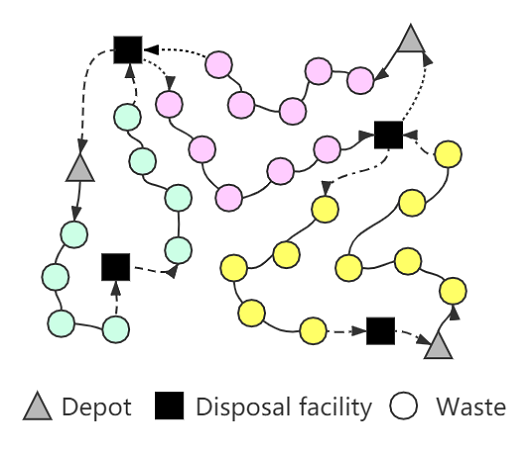
\includegraphics[scale=0.3]{PPSN2.png}
% \caption{A route sequence of one vehicle considering multiple disposal facilities and multiple depots. The different types of dotted lines connecting to disposal facilities represent different paths from different depots}
% \label{figl1}
 
%\end{figure}
%\todo[inline]{Formulation of classical CVRP: CVRPTW/ MDCVRP/ MTCVRP\\
%{\em need to add the citation of CVRPTW/ MDCVRP/ MTCVRP}}
%The vehicle routing problem (VRP) is a combinatorial optimisation and integer programming problem which provides vehicles with the best route to give service to different customers under given constraints ~\cite{dantzig1959vehicle}. The capacitated vehicle routing problem (CVRP) is a type of VRP, which adds an additional constraint to the classic VRP, that is, each vehicle has a limit capacity. With the limit capacity constraints, the vehicles need to pick up or deliver items at minimum cost without exceeding the capacity of the vehicle. 

%\todo[inline]{Check the format of references}
%\todo[inline]{Check if the acronyms ``ELS'' and ``MAELS'' have been defined before using them.}
%\todo[inline]{Change ``M3CWSA V I'' and ``M3CWSA V II'' into something simpler, such as ``M3CWSA-I'' and ``M3CWSA-II'' or ``M3CWSA1'' and ``M3CWSA2''}


\IEEEPARstart{T}{he} capacitated vehicle routing problem (CVRP) is a classic NP-hard combinatorial optimisation problem aiming at efficiently allocating several vehicles with limited capacity to serve different customers under some constraints~\cite{dantzig1959truck,lenstra1981complexity,eksioglu2009vehicle}. In recent years, numerous variants of CVRP considering different constraints have been derived and researched. Examples include, but not limited to, the capacitated vehicle routing problem with time-windows (CVRPTW)~\cite{baldacci2012recent}, the multi-depot capacitated vehicle routing problem (MDCVRP)~\cite{liu2010two}, and the multi-trip capacitated vehicle routing problem (MTCVRP)~\cite{mingozzi2013exact}. The CVRP and its variants have many inspiring applications in real life, such as green logistics~\cite{ubeda2011green}, drone delivery~\cite{dorling2016vehicle} and waste collection~\cite{kim2006waste}.

The waste collection problem (WCP) is an important and common real-world problem, which focuses on efficiently collecting and dumping waste in a city~\cite{beltrami1974networks}. Examples of the waste collection process are shown in Figure~\ref{fig:routes}. The WCP in real-life is challenging due to the numerous constraints defined by the multiple depots (parking lots), the multiple disposal facilities, the limited capacity of vehicles, the limited working duration, as well as the large number of collection sites. 
%Waste collection, in essence, can be considered a VRP~\cite{belien2014municipal}. However, unlike the traditional VRP, WCP is a real world problem which takes a lots of constraints into account.
In particular, with the continuous expansion of city size and increase of population, the coverage area of waste collection in the city becomes larger and larger. Therefore, it is necessary to schedule the routes reasonably and effectively to reduce the total mileage of vehicles, the working time and even the number of allocated vehicles, i.e., different types of costs. 
%It has often been formalised as a capacitated vehicle routing problem (CVRP)~\cite{dantzig1959vehicle,eksioglu2009vehicle}.
%The traditional WCP takes many constraints into account, such as time windows~\cite{minh2013memetic,buhrkal2012waste}, multiple intermediate disposal facilities (inter-depots)~\cite{Liu2012A}, multiple depots~\cite{shen2018multi}, and multiple trips~\cite{belien2014municipal}, etc. While many waste collection algorithms have been implemented in many real world situations,  it  is  likely that most waste collection algorithms are not capable of solving our large scale M3CVRP.

WCP has been formalised as different variants of CVRP, taking into account one of the following constraints alone: 
%the time windows~\cite{kim2006waste,minh2013memetic,buhrkal2012waste},\todo{We don't consider time windows, but we still cite 3 articles here. JL: you can comment the time-window ones.} 
multiple depots~\cite{Gruler2017Supporting}, multiple intermediate disposal facilities (inter-depots)~\cite{Liu2012A} and multiple trips~\cite{belien2014municipal}.
However, to the best of our knowledge, none of the existing work has considered multiple depots, multiple disposal facilities and multiple trips at the same time. Thus, the methods and techniques designed for those existing models are not directly applicable to the large-scale multi-depot multi-disposal-facility multi-trip capacitated vehicle routing problems (M3CVRP) in real life.
%\todo[inline]{Briefly present the state of the art and limitations }
%This is because they do not consider so many constraints in a WCP. Once there are more constraints, many original good algorithms and frameworks need to be redesigned. 
%The collection and transportation process considered in this paper is shown in Figure~\ref{figl1} (Three different types of dashed lines represent three different routes). 
To fill the gap between the current research and the need of real-world applications, in this paper, we propose M3CVRP (Section~\ref{sec:m3cvrp}), a new and more realistic model, and perform a case study on a real-world problem with $3,000$ collection sites inside and around the Qingdao city of China (Section~\ref{sec:rwproblem}). 

\begin{figure}[htbp]
\centering
\begin{subfloat}[\label{figl}Trips considering multiple disposal facilities with one single depot. The dashed lines refer to the paths from waste collection sites to the closest disposal facilities and vice versa.]{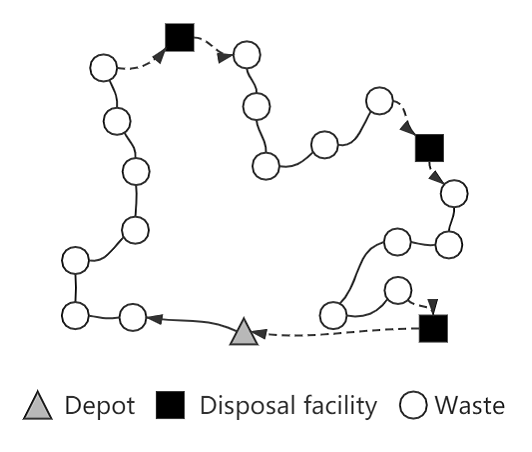
\includegraphics[width=.23\textwidth]{PPSN1.png}}
\end{subfloat}\hfill
\begin{subfloat}[\label{figl1} 
Trips considering multiple disposal facilities with multiple depots. Different types of dashed lines refer to the paths belonging to different routes. ]{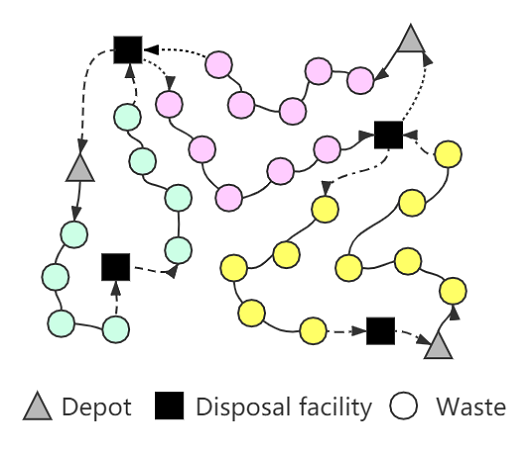
\includegraphics[width=.23\textwidth]{PPSN2.png}}
\end{subfloat}
\caption{\label{fig:routes}Examples of routing plans for vehicles. The solid lines refer to the paths between two different waste collection sites or the paths from the depot to the closest waste collection site.}
\end{figure}

The features of the real-world WCP studied in this paper (detailed in Section~\ref{sec:problem}) are summarised as follows. 
\begin{enumerate}[leftmargin=*,label=(\roman*)]
\item \emph{Large-scale}: $3,000$ collection sites are considered. As a result, many traditional methods for small datasets will no more be suitable or take too much time to find a satisfactory solution. 
\item \emph{Multi-depot}: for the practical issue, each collection site can be recycled by waste vehicles from different depots. 
\item \emph{Multi-disposal-facility}: a fully-loaded vehicle can dump in different disposal facilities. 
\item \emph{Multi-trip}: vehicles can carry out the process of waste collection, transportation, and dumping multiple times before returning to the depot.  
\item \emph{Limited maximum working time}: vehicles cannot keep collecting all day long. 
\end{enumerate}
Figure~\ref{figl1} demonstrates an illustrative example of a multi-depot multi-disposal-facility multi-trip route.

The considered WCP is confronted with more challenges due to being closer to real-life scenarios. The multi-depot, multi-trip and multi-disposal-facility features result in the requirements of complex considerations with more constraints. Moreover, a large number of collection sites leads to an increase of search space which consumes more time for evaluating solutions and searching for optimal solutions. 
%We can only obtain insufficient real world information, such as: we do not know if the waste collection site is on the same path or not which make it difficult to simplify the problem, etc. 

To tackle these extremely complex features and challenges presented above, new problem model and efficient heuristics are needed to boost the optimisation. The main contribution of this work as as follows. 
\begin{enumerate}[leftmargin=*,label=(\roman*)]
\item We formalise a more realistic model for real-world waste collection problem, namely M3CVRP (Section~\ref{sec:m3cvrp}). 
\item We propose a novel heuristic-assisted solution initialisation algorithm (HaSI) for generating solutions of high quality (Section~\ref{sec:hasi}).
%(ii) We propose a novel two-phase route optimisation approach consisting of a heuristic-assisted solution initialisation algorithm (HaSI) for generating solutions of high quality (Section~\ref{sec:hasi}) and an extended local search (ELS, Section~\ref{sec:els}) as an efficient optimiser;
\item We also design an extended local search (ELS) as an efficient optimiser, the core components of which are two region-constrained swap operators and a relaxed multi-point swap operator (Section~\ref{sec:els}). 
\item In particular, a new disposal facility (inter-route depots) insertion with the backspacing method, which further improves the mileage when completing solutions for evaluation (Section~\ref{sec:bsim}), is proposed.
\end{enumerate}
%(v) We adapted the MA framework to further improve the optimisation process. (iv)
To the best of our knowledge, no one has ever considered such a large-scale problem, we have given a direction to deal with such issues. Our proposed approach can be extended to other routing problem with the same number of or fewer constraints.

\def\toolong{
\begin{enumerate}
%    \item We add some randomness to the traditional greedy algorithm to generate initial solutions of high quality and increase the diversity among individuals.
    \item We design two new space-constrained swap operator and a new multi-point swap operator. 
    \item We propose a disposal facility (inter-route depots) insertion with backspace method.
    \item We adapted the MA framework to further improve the optimisation process.
    %\todo{If we still need this? We did not modify the MA framework, we just applied our local search}
    \item To the best of our knowledge, no one has ever considered such a large-scale problem, we've given a direction to deal with such problems.
    \item Our proposed approach can be approximated as a CVRP with the same number of or fewer constraints.
\end{enumerate}}
% an adaptive memetic algorithm (MA) with improved operator of local search as an efficient optimiser (Section~\ref{sec:two_phase})

\def\oldversion{In this paper, the features of the problem proposed can be represented by the following points:
\begin{enumerate}
    \item Large scale problem which means that many traditional methods for small dataset won't suit for this problem or need to take so much time.
    \item Multiple disposal facilities and multiple depots. Because this is a practical issue, each waste point can be recycled by waste vehicles in different parking lots. After the waste vehicle is full of waste, you can choose different disposal facilities to dump.
    \item Multiple trip means that the waste vehicle can complete the process of collecting, transporting, and dumping waste multiple times within a specified time.
    \item Vehicles can only work during the time restraint.
\end{enumerate}}

\def\oldversion{Because this is a realistic problem, coupled with the above features, the problem has the following challenges:
\begin{enumerate}
    \item The 3000 collection sites make the search space extremely large, which requires a lot of time to optimise. 
    %\item challenge2: The traditional MA framework is only applicable to CARP but not CVRP. How to effectively apply the MA framework to CVRP is also a challenge.
    %\item challenge2: Because it is a practical problem, we often need to consider the degree of load balance between vehicles and whether the paths arranged by each vehicle are compact.
    \item We can only obtain insufficient real world information, such as: we do not know if the waste collection site is on the same path or not which make us difficult to simplify the problem, etc.
    \item As a realistic problem, it is more complicate and with more constraints need to consider, including multi-depot, multi-trip and  multi-disposal-facility.
\end{enumerate}}

\def\oldversion{Out of the above-mentioned challenges and features of the problem, we mainly did the following work:
\begin{enumerate}
    \item We add some randomness to the traditional greedy algorithm to generate the initial solution population. The randomness we add here is to make the population diverse.
    \item We propose a new space-constrained swap operator which is better then the traditional swap operator in our problem.
    \item No one has ever considered such a large scale problem, We have given a direction to deal with this problem.
    \item The approach proposed in this paper can be approximated as a CVRP with same or less kind of constraints.
    \item We adaptive the MA framework to further perform algorithm optimisation.
\end{enumerate}
As we have seen, this is an extremely complex real-world problem with multi-depot, multi-trip and multi-disposal-facility constraints, and it is difficult to simplify. We used hierarchical approach including the heuristic-assisted population initialisation algorithm in the first part and adaptive MA together with improved operator of local search in the second part to do the experiments on this problem.
}
%\todo[inline]{Describe the problem (one paragraph){\em Needs to highlight the %unique features of this problem: real-world, large-scale, multiple depots, %multiple dumping sites, multiple trips by one vehicle, etc.}}


The rest of this paper is organised as follows. Section~\ref{sec:background} discusses the related work. Section~\ref{sec:problem} describes the real-world WCP and gives the mathematical formulation of M3CVRP. The details of proposed HaSI and corresponding experimental study are presented in Section~\ref{sec:initial_solution}, while Section~\ref{sec:optimisation_mathod} presents our ELS and corresponding experimental study. Finally, Section~\ref{sec:conclusion} concludes and points out some potential future directions.


%===========================  第  二  段  ===================================
\section{Background}\label{sec:background}
%In this section, the brief survey of research method related to this paper is provided. We start from the CVRP and the CARP implemented in WCP, and then describe the common move operators using in local search.

\subsection{Related Work}%Optimisation Methods for WCP}
Dantzig and Ramser~\cite{dantzig1959truck} first introduced the vehicle deliver problems and modelled such problems as CVRP. However, a general CVRP is a simplified model and many constraints in real life are not considered. At the early stage of research around CVRP, exact methods were often used to search for optimal solutions~\cite{baldacci2012recent, martello2000three}. Nevertheless, almost all exact methods are only suitable for optimising problems of small size and suffer from the curse of dimensionality~\cite{martello2007algorithm,akhtar2017backtracking}. The search space of CVRP increases exponentially when the problem dimension increases. Exact methods can hardly find optimal solutions in an acceptable time when the problem size is huge. Hence, heuristic methods are widely used to solve CVRPs approximately~\cite{taillard1999heuristic,tan2001heuristic,laporte2002classical}. 

Beltrami and Bodin~\cite{beltrami1974networks} applied the Clarke and Wright (CW) algorithm~\cite{clarke1964scheduling} to solve waste collection problems where the tasks are located on nodes. Pichpibul and Kawtummachai~\cite{pichpibul2012an} improved the CW algorithm by changing traverse order of savings list with the mechanism of tournament and the roulette wheel selection. Meta-heuristics have also been applied.
%For instance, Melo \emph{et al.}~\cite{melo2017optimization} applied a genetic algorithm (GA) to waste collection problems and examined how the likelihood of mutation and crossing will influence the \textcolor{red}{iteration times.}\todo{generation number?}
In the work of Mi \emph{et al.}~\cite{mi2017optimization}, the nearest neighbour's algorithm (NNA) was implemented to generate initial solutions for genetic algorithm (GA).
Kim \emph{et al.}~\cite{kim2006waste} focused on solving large-scale waste collection problems with one single depot and $2,100$ tasks by a capacitated clustering-based waste collection VRPTW algorithm. He and Liu~\cite{Liu2012A} divided a multi-depot VRP into several sub-problems through clustering, and then solved each sub-problem by an ant colony separately. Memetic algorithm (MA), first introduced by Moscato \emph{et al.}~\cite{moscato1989evolution}, is another popular meta-heuristic for solving VRPs. Minh \emph{et al.}~\cite{minh2013memetic} adapted MA with partial-mapped crossover operator to generate offspring and $\lambda$-interchange operator in local search. Akhtar \emph{et al.}~\cite{akhtar2017backtracking} focused on solving the dynamic urban waster collection problem in which the volume of waste at each collection site can be detected in real-time through sensors. Benjamin and Beasley~\cite{benjamin2013metaheuristics} noticed the perturbation to the quality of solution caused by the insertion of disposal facilities, especially when multiple trips occur. A disposal facility positioning (DFP) algorithm was proposed to search for proper positions for inserting the disposal facilities~\cite{benjamin2013metaheuristics}.

The work reviewed previously modelled the WCPs as variants of CVRP. WCP has also often been modelled as variants of capacitated arc routing problem (CARP)~\cite{tang2009memetic,mei2013decomposing,mei2014cooperative,tang2017scalable,akhtar2017backtracking,mi2017optimization}. 
%Mei~\emph{et al.}~\cite{mei2013decomposing} considered large-scale CARPs and designed decomposition methods to reduce the solution space and computational time. 
Decomposition methods have been designed for handling large-scale CARPs, such as the random route grouping (RGG) and the route distance grouping (RDG)~\cite{mei2013decomposing}. The variable neighborhood decomposition (VND)~\cite{mei2014cooperative} was implemented within the cooperative co-evolution (CC) framework so that the decomposition can be adjusted dynamically. 
%Mei~\emph{et al.}~\cite{mei2014cooperative} combined the VND and MAENS using a merge-split operator proposed in~\cite{tang2009memetic}.with larger step-size than typical operators to escape from the local optimum. 
More recently, a scalable approach based on hierarchical decomposition (SAHiD) was proposed by Tang \emph{et al.}~\cite{tang2017scalable}. 
%SAHiD outperformed the algorithms presented previously on real-world large-scale CARPs with thousands of tasks.
%为什么提到的算法或模型不能适用于这个问题? 因为以往的算法都没有处理过这么大规模的问题,因此无法保证算法可以直接用于该问题,或者能够继续保持良好的运行结果。 

Most of the existing work on CVRP and CARP focused on solving problems with dozens of  collection sites, while the number of collection sites in our case is much higher. Kim \emph{et al.}~\cite{kim2006waste} solved a vehicle routing problem with time windows (VRPTW) with $2,100$ collection sites but still far fewer than ours. Therefore, existing algorithms may not be directly applicable to our large-scale problem and the existing decomposition methods may fail due to a large number of tasks to be clustered.
%So it is uncertain whether these proposed and tested algorithm can work on such a large scale problem. 
%Mei has proposed RDD, RDG and VND under CC framework to solve large scale CARP~\cite{mei2013decomposing}~\cite{mei2014cooperative}~\cite{mei2014cooperative}.
Only SAHiD was applied to a problem of 3,584 tasks~\cite{tang2017scalable}. Nevertheless, how to apply SAHiD to our real-world UWCP is not evident as the SAHiD was designed for CARP with one single depot (which is at the same time a disposal facility), while in our case, multiple depots and multiple disposal facilities are involved. 

\subsection{Classical Search Operators in Local search}\label{move_operator}

%\yzy{A candidate solution is often conducted by applying search operators on one or more an original solution as input~\cite{tang2009memetic}.
Search operators is one of the core components of local search algorithms. A good number of search operators have been designed for routing problems with different constraints.
Some popular search operators, such as insertion, swap and 2-opt~\cite{lin1965computer}, have been widely extended~\cite{handa2006robust,handa2006robust2,hertz2000a,hertz2001a,BeullensA,brandao2008a}. Song and Dong~\cite{song2018an} adopted swap and 2-opt to solve CVRP by embedding local search (LS) with these two search operators into differential evolution (DE) algorithm. The CROSS-exchange, first proposed by~\cite{golden1980approximate}, was adapted to swap segments of consecutive waste collection sites between two routes, and was embedded with tabu search to solve the vehicle routing problem with soft time windows (VRPSTW)~\cite{taillard1997a}. Kim \emph{el al.} applied CROSS-exchange to single routes in simulated annealing (SA) algorithm 
in order to improve the sub-route construction performance of the waste collection vehicle routing problem with time windows (VRPTW)~\cite{kim2006waste}. 
%\todo[inline]{cannot find the paper from the following citation}
%\lwx{Br\"aysy proposed IOPT-operator~\cite{braysy2001local}, a modification of CROSS-exchanges, to local search for solving VRPTW. 
GENICROSS operator, which draws upon GENIUS insertion heuristic~\cite{gendreau1992new} and CROSS-exchanges, and IOPT-operator~\cite{braysy2004a} were used to optimise VRPTW~\cite{braysy2004a}. Three neighbourhood operators, denoted as $N_1$, $N_2$ and $N_3$, were adopted by Zhou and Wang to solve multi-objective vehicle routing problem with time windows~\cite{zhou2015a}. Particularly, $N_1$, similar to insertion operator, randomly selects a waste collection site from a route and re-inserts it into the best position of the same route~\cite{zhou2015a}. The difference between $N_2$ and $N_1$ is that $N_2$ removes a random number of waste collection sites rather than one and $N_3$ exchanges a sequence of sites with the same orientation and the same order~\cite{zhou2015a}. 
%\todo[inline]{Jialin: why discussing N1, N2 and N3 in details here? Did they inspire our work?}
%\todo[inline]{Jialin: Needs a sentence to close the above section, the following one is a draft}
The search operators mentioned above except the ones in \cite{zhou2015a} may be not suitable to large-scale M3CVRP. Since these search operators with greater randomness cannot obtain better solutions efficiently. 
%The ones in \cite{zhou2015a} are not directly applicable to our problem neither due to more constraints being involved.

\section{Real-world Waste Collection Problem}\label{sec:problem}

\subsection{Problem Description}\label{sec:rwproblem}
% 如何获取距离、我们有哪些数据(id\lng\lat....)

Our case study is based on a real-world WCP of $3,000$ collection sites, $3$ disposal facilities and $3$ depots located inside and around the Qingdao city of China. It is worth mentioning that one of the depots is at the same time a disposal facility. Thus, there are $3,005$ locations (or nodes) in total. Figure~\ref{fig:dataset} visualises the distribution of locations. As a realistic problem, the dataset of this problem is extremely large, which consists of thousands of waste collection sites, multiple depots and multiple disposal facilities. It is not trivial to solve such a complex problem. 
%as many recent publications on CVRP or UWCP~\cite{akhtar2017backtracking,mi2017optimization,minh2013memetic} only considered problems of dozens or hundreds of collection sites. 
As the problem grows in size and complexity, the size of the solution search space grows exponentially, and the difficulty of finding a good solution also increases significantly. In addition, the WCPs with several depots and several disposal facilities have rarely been discussed in existing work (cf. Section \ref{sec:background}). 

%The most essential information is the distance between any two vertices including waste collection sites, disposal facilities and depots. After getting the latitude and longitude of the points, the distance between any two vertices was determined as the distance of the driving routes planned by Gouda API. Hence, the distance from a vertex $i$ to vertex $j$ does not always equal to the one from $j$ to $i$ due to single lanes. 

A vehicle is allowed to collect waste at one or more collection sites under the condition that its load does not exceed its capacity. A vehicle can empty its load to any disposal facility, and then start a new trip, which will lead to multiple trips to disposal facilities or return to its depot. The aim of solving WCP is to find a set of routes that satisfies the constraints listed below.
\begin{enumerate}[label=$\mathcal{C}_\arabic*$:]
    \item Each vehicle starts and ends at the same depot at the beginning and end of the day, respectively.
    \item Each waste collection site should be served exactly once by exactly one vehicle.
    \item The load of any vehicle at any moment cannot exceed its capacity.
    \item No vehicle is allowed to work longer than its legal working time.
    \item The load of any vehicle leaving a depot or a disposal facility should be $0$.
\end{enumerate}

\begin{figure}[htbp]
\centering
	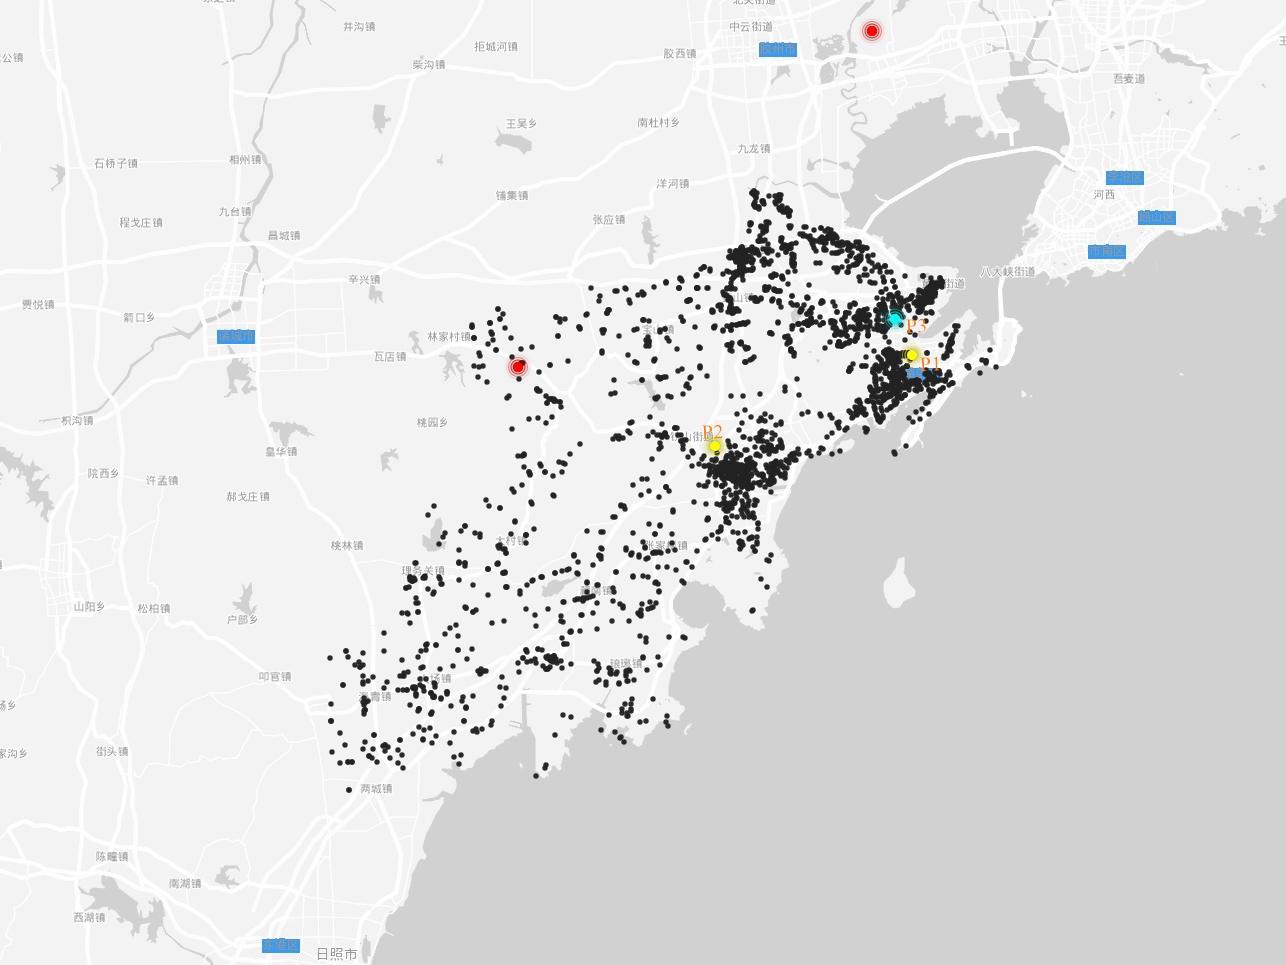
\includegraphics[width=0.49\textwidth]{dataset_new.png}
	\caption{\label{fig:dataset}
	The visualisation of depots (red points denoted as $P_1$, $P_2$ and $P_3$), waste collection sites (black points) and disposal facilities (yellow points) on real-world map. The cyan-blue point refers to the depot that is also a disposal facility.}
\end{figure}

\subsubsection{Data Collection and Pre-processing}\label{sec:data}
The identity, volume of waste, location (latitude and longitude) and service cost of each collection site are given in the dataset, as well as the name, identity and location of depots and disposal facilities. The service cost of each disposal facility is set as $0$ since there is no such data in the original dataset. The distance from any location $A$ to location $B$, denoted as $dist(A,B)$, was not given in the original dataset, but determined as the distance of driving route from $A$ to $B$ calculated by a public API of \emph{AutoNavi}\footnote{\url{https://lbs.amap.com/api/javascript-api/guide/services/navigation}}. Note that $dist(A,B)$ does not always equal to $dist(B,A)$ due to single lanes. Previous work rarely considered such kind of situation.


%These features make the problem more complicate which result in potential multi-trip to disposal facilities.

\subsubsection{Necessity of a New Model}\label{sec:discussmodel}

Compared with existing work on VRPs, the characteristics of our model include multiple depots, multiple disposal facilities and the limitation on the working time of each vehicle. To the best of our knowledge, VRPs with multiple disposal facilities (inter-route depots) are rarely considered. Most work only considered one single disposal facility, which is, at the same time, the only depot in their dataset~\cite{bautista2008solving,tang2017scalable,akhtar2017backtracking,mi2017optimization}. Multiple trips are usually caused due to multiple disposal facilities, and make the problem more complicated as it is necessary to consider the selection and insertion of disposal facilities in a route~\cite{kim2006waste,benjamin2010metaheuristics,buhrkal2012waste}. Existing solutions to tackle the problem with multiple depots usually consider converting it into problems with single depot by clustering or classification of collection sites~\cite{kim2006waste,shi2020heuristic}.

The issues and drawbacks of applying directly existing models to our real-world problem are summarised below.
\begin{itemize}
\item Scalability issue: Most of the current research work on small- or middle-size datasets which contain fewer than $1,000$ points. When dealing with large datasets, the issue of the dimensional explosion may happen. For instance, when using CPLEX to solve TSP, the memory required increases exponentially with the increase of the number of points, owing to the fact that the number of decision variables and constraints has significantly increased~\cite{crevier2007multi, babaee2019developing}. Thus, if using CPLEX for solving our problem with $3,000$ sites, at least 12TB of memory and several days of runtime are required to find a feasible solution, which is not acceptable in the real-world situation.
\item Unpractical Euclidean distance: Actual travelling distance between locations is rarely considered in existing work, while Euclidean distance is mostly used~\cite{kim2006waste,Han2015WASTE,rabbani2016hybrid}. However, in real life, two points with short Euclidean distance may be very far apart, as, for example, there is a river between these two points.
\item Legal working time: In real-world scenarios, the maximum working time of vehicles should be taken into account. In other words, no vehicle is permitted to collect and transport waste indefinitely~\cite{tirkolaee2018robust}.
\item Multiple depots and multiple disposal facilities: For large cities (e.g., Shenzhen and Los Angeles), there are usually many disposal facilities and depots. With the acceleration of urbanisation, the model of single depot or single disposal facility~\cite{babaee2019developing,wu2020optimization} will become less and less applicable.
\end{itemize}
Therefore, a new problem model considering all above is necessary.

\subsection{M3CVRP}\label{sec:m3cvrp}

To handle the WCP described above, we formalise a novel mathematical model,  multi-depot multi-trip multi-disposal-facility capacitated vehicle routing problem (M3CVRP). The city and surrounding area can be regarded as a directed graph $G=(V,E)$, where $V$ is the vertex set and $E$ is the edge set. The vertex set $V$ is the union set of the set of depots ($V_P$), the set of waste collection sites ($V_C$), and the set of disposal facilities ($V_D$). It is notable that in our real-world WCP, one of the disposal facility is also a depot which is often the case for other cities, i.e., $V_P \cap V_D \neq \emptyset$ and $V_P \neq V_D $. Each collection site $c \in V_C$ has a non-negative amount of waste $t(c)$ to be collected and a non-negative service time $\delta(c)$. Disposal facilities and depots have no waste and no service time is consumed in depots in our practical application, so the $t(p)$ is set as $0$ for $p\in V_P \cup V_D$, and $\delta(p)$ is set as $0$ for $p\in V_P$. Every disposal facility has an infinite capacity which means that $\forall d \in V_{D}$ can be visited for an infinite number of times. The edge set $E$ is defined as $\{(i,j)\mid \forall i,j \in V, i \ne j\}$ and the distance from vertex $i$ to vertex $j$ is denoted by $dist(i,j)$. $M$ denotes the number of vehicles. Each vehicle $v$ has a limited capacity $Capacity(v)$, a moving speed $Speed(v)$, and maximum legal hours of work in a day $WT(v)$. Furthermore, $Load(v,i)$ indicates that the load of $v$ at vertex $i$, where $i\in V$.

We formulate each solution $S$ as a set of distinct routes $\{R_1,\dots,R_{M}\}$, where $R_{k}$ is the route served by the vehicle $k$, $\forall k \in \{1, \dots M\}$.
% $\forall k \in \{1,\dots,M\}$. 
Each $R_k$ is associated to one and only one depot denoted by $p_k$, which implies constraint $\mathcal{C}_1$.
Each route consists of several trips and is formalised as $R_{k}=\{r_{k,1},\dots, r_{k, l_k}\}$, where $l_k$ is the number of trips in route $R_{k}$. One or more disposal facilities inserted to the route $R_{k}$ are referred to as $d_{k,1}, \dots, d_{k,l_k}$. It is possible that a disposal facility is visited more than once in a route or only one disposal facility is visited in a route.
The $i^{th}$ trip served by the $k^{th}$ vehicle, $r_{k, i}$, can be represented as a sequence $(c_{k,i,1},\dots, c_{k,i,h_{k,i}})$, where $c_{k,i,1},\dots, c_{k,i,h_{k,i}} \in V_C$ are the collection sites allocated to this trip and $h_{k,i}$ is the number of served collection sites in this trip. $Set_c(r_{k, i})$ denotes the set of collection sites in $r_{k, i}$. Therefore, $|Set_c(r_{k, i})|=h_{k,i}$ as each site is collected exactly once.
%The first trip should start from a depot and the last one should return to the same depot, while the other trips begin and end at disposal facilities. 
%Thus, when $i$ is 1, $c_{k,1,0} \in V_P$, $j\in V_P \cup V_D$; when $i=l_k$, $c_{k,l_{k},1+h_{k,i}} \in V_P$; otherwise $c_{k,i,0},c_{k,i,1+h_{k,i}}\in V_P\cup V_D$.
%$i, j\in V_P\cup V_D$ (If $m=0$, $i \in V_P$. If $m=l$, $j \in V_P$.).
A vehicle has an empty trip set if no task has been assigned to it.
%\rc{\em Second, we give the mathematical model}
%\todo[inline]{Formalise your model. Given clear notations and use them in the rest of this paper. Part of your  final report can be used here.}
% which means the total working time of $v$ cannot exceed $WT(v)$.
%Let $Load(v,i)$ denote the load of vehicle $v$ when leaving vertex $i$, $\forall i\in V$. 
%Let $dist(A)$ and $time(A)$ denote the total distance and time cost of $A$, respectively. $A$ can be either a route or a solution.
The shortest path between any pair of vertices is assumed to be available or calculable.
\def\removed{
Therefore, we define directly variables $x_{i,j,v}$ ($v \in M$ and $i,j\in V$) to indicate if the vehicle $v$ travels from the vertex $i$ to the vertex $j$. Thus, $x_{i,j,v}=1$ if yes, otherwise $x_{i,j,v}=0$.
The objective of M3CVRP is minimising the total travel distance of all allocated vehicles, formalised as follows.
}
% and minimising the number of allocated vehicle. 
% These two objectives are converted to a single objective function, $F$, to be minimised using a linear combination, formalised as follows.
%The objective is converted to a single objective function, $F$, formalised as follows.
%\linespread{1.5}
%\begin{table}[htbp]
%	\caption{Symbol Table}
%	\begin{tabular}{l p{10.8cm}}
%		\hline
%		Symbol & Definition \\
%		\hline
		% $\vert A\vert$ & Represents the cardinality of the set A. A is any set. \\
	%	$\| \alpha \|$ & If condition $\alpha$ is true, the statement will be 1. Otherwise, it will be 0. \\
		% $max(A)$ & The maximum value in the set A. A is any set. \\
		%$V_P$ & The set of depot can be regarded as $V_P=\{p_0, p_1, ..., p_k\}$. \\
	%	$V_C$ & The set of collection sites can be regarded as $V_C=\{c_0, c_1, ..., c_k\}$. \\
	%	$V_D$ & The set of disposal facilities can be regarded as $V_D=\{d_0, d_1, ..., d_k\}$. \\
	%	$V$ & The set of all vertexes can be regarded as $V = V_P \cup V_C \cup V_D$. \\
	%	$E$ & Directed edge set between any two vertexes $i$ and $j$, where both $i, j\in V$. \\
	%	$G$ & The directed graph can be regarded as $G=(V, E)$. \\
	%	$dist_{ij}$ & The distance between two vertexes $i$ and $j$(The distance refers to the actual driving distance planned by using the Gouda API). If there is no route from $i$ to $j$, the distance will be infinity, where both $i,j\in V, i \neq j$. \\
		%$M$ & The set of vehicles can be regarded as $M=\{v_0, v_1, ..., v_k\}$. \\
	%	$Capacity(v_k)$ & The maximum capacity of the vehicle $v_k$, where $v_k \in M$. \\
	%	$Load(v_k,i)$ & The load of vehicle $v_k$ at $i, i\in V$.\\
	%	$WT(v_k)$ & The longest time which the vehicle $v_k$ can work, where $v_k \in M$. \\
	%	$t_k$ & The volume of the waste in collection site $c_k$, where $c_k\in V_C$. \\
		%$\delta_{c_k}$ & The time cost of collecting the waste in collection site $c_k$, where $c_k\in V_C$. \\
	%	$Speed(v_k)$ & The average speed of the vehicle $v_k$, where $v_k \in M$. \\
		%$R_{v_k}$ & The set of the trips of the vehicle $v_k$ during its working time which is $R_{v_k}=\{R_{v_k,0_k}, R_{v_k, 1_k}, ..., R_{v_k, l_k}\}, l$ is the number of trips of vehicle $v_k$. \\
		%$R_{v_k, m_k}$ & The $m$-th trip of the vehicle $v_k$ and $R_{v_k, m_k} \in R_{v_k}$, which is $R_{v_k,m_k} = \{i, c_{\alpha_0}, c_{\alpha_1}, ..., c_{\alpha_h}, j\}, i,j\in V_P\cup V_D$ (If $m=0$, $i \in V_P$. If $m=l$, $j \in V_P$.), $c_{\alpha_0}, c_{\alpha_1}, ..., c_{\alpha_h}\in V_C$, $h$ is the number of waste collection point in this trip. \\
%		$x_{i,j,k}$ & If vehicle $v_k$ travels from vertex $i$ to $j$, the $x_{i,j,k}$ will be 1, otherwise 0, where $v_k\in M, i,j\in V$. \\
	%	$S$ & One solution of problem. $S = \{R_{v_0}, ..., R_{v_k},...\}, v_k \in M.$\\
%		$dist(A)$ & The total distance of $A$, $A$ can be route or solution\\ 
%		$time(A)$ & The total time cost of $A$, $A$ can be route or solution\\
	%	$Y$ & The set of using vehicle number in solution $S$ \\
%		\hline
%	\end{tabular}
%\end{table}
The distance of the $i^{th}$ trip of vehicle $k$, including travelling from/to the disposal facilities, is calculated as
\begin{equation}\label{eq:ct}
\begin{split}
    C_{t}(r_{k,i}) = & dist(d_{k,i-1},c_{k,i,1}) + \sum_{j=2}^{h_{k,i}} dist(c_{k,i,j-1},c_{k,i,j}) \\
    &+ dist(c_{k,i,h_{k,i}},d_{k,i}),
    \end{split}
\end{equation}
where $dist(d_{k,0},c_{k,1,1})=0$.
Then, the distance of the route of vehicle $k$, including travelling from/to the depot $p_{k}$, is calculated as 
\begin{equation}\label{eq:cr}
C_r(R_k)=dist(p_k,c_{k,1,1}) + \sum_{i=1}^{l_{k}} C_{t}(r_{k,i}) + dist(d_{k,l_k},p_k).\hspace{-3pt}
\end{equation}
If $d_{k,l_k}$ is identical to $p_k$, thus the visited disposal facility is also a depot, then $dist(d_{k,l_k},p_k)=0$. 
The objective of M3CVRP is minimising the total travel distance of all allocated vehicles, formalised as \eqref{eq:cost}. The constraint $\mathcal{C}_1$ (described in Section \ref{sec:rwproblem}) is implied in the objective function \eqref{eq:cost}. The constraint $\mathcal{C}_2$ is ensured by \eqref{eq:tasknb1} and \eqref{eq:tasknb2}. The constraints $\mathcal{C}_3$, $\mathcal{C}_4$ and $\mathcal{C}_5$ are explicitly ensured by \eqref{eq:capacity}, \eqref{eq:time} and \eqref{eq:load}, respectively.

\begin{figure*}[h!]
\begin{equation}\label{eq:cost}
\min ~ Cost(S) = \sum_{k=1}^{M} C_r(R_k),
\end{equation}
\begin{eqnarray}
S.t. &&  p_{k}\in V_{D}\text{, } \forall k\in\{1,\dots, M\}\text{, }\nonumber\\
&& d_{k,i}\in V_{D}\text{, } \forall k\in\{1,\dots, M\}\text{, }\forall i\in\{1,\dots, l_k\}\text{, } \nonumber\\
%&& S.t.  p_{k}\in V_{D}\text{, } \forall k\in\{1,\dots, M\}\text{, } \label{eq:depot}\nonumber\\
%&& d_{k,i}\in V_{D}\text{, } \forall k\in\{1,\dots, M\}\text{, }\forall i\in\{1,\dots, l_k\} \label{eq:df}\nonumber\\
&& c_{k,i,j}\in V_{C}\text{, } \forall k\in\{1,\dots, M\}\text{, } \forall i\in\{1,\dots, l_{k}\} \text{, } \forall j\in\{1,\dots, h_{k,i}\},\nonumber\\
&& \cup_{k=1}^{M} \cup_{i=1}^{l_{k}} Set_c(r_{k,i})=V_C, \hspace{-3pt}\label{eq:tasknb1}\\
&&\sum_{k=1}^M\sum_{i=1}^{l_k} |Set_c(r_{k,i})|=|V_c|, \hspace{-3pt}\label{eq:tasknb2}\\
 &&\sum_{j=1}^{h_{k,i}} t(c_{k,i,j}) \leq Capacity(k) \text{, }\forall k\in\{1,\dots, M\}\text{, } \forall i\in\{1,\dots, l_{k}\}, \label{eq:capacity} \\
&&\frac{C_r(R_k)}{Speed(k)} + \sum_{i=1}^{l_{k}} \left(\sum_{j=1}^{h_{k,i}} \delta(c_{k,i,j})+\delta(d_{k,i})\right)  \leq WT(k)\text{, }\forall k\in\{1,\dots, M\},\label{eq:time}\\
&& Load (k, p_k) = 0\text{, }\forall k\in \{1,\dots,M\}\text{, } p_k\in V_P.\label{eq:load}
%&& Load(v,p)=0\text{,  } \forall v\in M, \forall p\in V_P\cup V_D\label{eq:empty}
\end{eqnarray}
\end{figure*}

%The objective function \eqref{eq:cost} indicates the minimisation of total travel distance, followed by the additional constraints.
%The constraint that the amount of waste of a trip should not exceed the vehicle's capacity is imposed in \eqref{eq:load}.
%\todo{you have used $t_k$ to refer to the volume of the waste in collection site but now you are using $n$} 
%\todo[inline]{check the model and constraints.}
%It's not necessary to explicitly indicate the constraint $\mathcal{C}_5$ (i.e., $0$ load when leaving a depot or a disposal facility) here.
%\eqref{eq:time} indicates that no vehicle can work longer than its maximum working time. %\eqref{eq:empty} indicates that the load of any vehicle leaving form any depot or disposal facility should be $0$.

In this M3CVRP model, multiple depots, multiple disposal facilities, multiple trips, the working hours of each vehicle, the service time of each site and capacity constraints are simultaneously considered, which makes the model extraordinarily complicated but closer to a real-world situation.

%\subsection{Necessity of New Algorithms}

%\rc{\em Third, we point out again the unique features of this model, which is different from all previous models.}
	
%\todo[inline]{the variants of routing problems modelled for waste collection in research, in particular, the one with time windows (pages 8, 10 of the slides of your viva last semester)}
%相较于其他WCP或者CVRP模型的特殊之处
%\todo[inline]{Compare this section to Section~\ref{sec:discussmodel}, and moving model related discussions to Section~\ref{sec:discussmodel}. This section should talk about methods.}


%\todo[inline]{Introduce the some of the related state-of-the-art of research  (pages 9, 11 of the slides of your viva last semester), not only CVRP but also CARP}
%CVRP的stat-of-art,在查阅文献时主要考虑:1.解决问题的size 2.数学模型的区别 (约束条件的区别)3.解决的方法
%\todo{can we delete the blue sentences?}

%\checkthis{If we want to formulate our problem into CARP, it need to figure out that what waste collection sites are in a same arc.}
\def\toolong{What's more, it's hard to model our UWCP as a CARP, as the information of roads is not available from our original data, thus it's not possible to construct arc between any two vertices.} 
%as mentioned previously, it's not possible to figure out what \todo{Jialin: i have not finished this sentence.} we cannot obtain these information just start from our original data.


%\todo[inline]{Detail how the quality of solutions will be measured}
%解的评估方式
%The main objective in this problem is to minimize the total distance of vehicles, and we will also consider the number of vehicle used to solve the problem. Since there is few paper focus on the same problem as ours and with enough large problem size and also with drivers' time constraint. In this paper, we measure the quality of algorithm not only by solution's total distance and the number of used vehicles by also the its robustness and the computation time of optimisation. 

\section{Smart Initialisation}\label{sec:initial_solution}
In this section, we propose a heuristic-assisted approach (Section~\ref{sec:hasi}) to generate initial solutions of high quality efficiently. The representation of the initial solution is given in Section~\ref{init_sr}. An adaptation of Clarke and Wright Savings Algorithm (CWSA) (Section~\ref{m3_cwsa}) \cite{clarke1964scheduling} is employed as a baseline algorithm in the initial solution construction. Experimental study and discussion are presented in Section~\ref{init_es} and Section~\ref{sec:init_discuss}, respectively.

\subsection{Solution Representation}\label{init_sr}
An initial solution is represented as an ordered permutation of tasks, depots and disposal facilities. For instance, the route of vehicle $k$ is presented as: $p_k\rightarrow c_{k,1,1} \rightarrow c_{k,1,2} \rightarrow \cdots \rightarrow c_{k,1,h_{k,l}} \rightarrow d_{k,1} \rightarrow c_{k,2,1} \rightarrow \cdots \rightarrow c_{k,l_k, h_{k,l_k}} \rightarrow d_{k,l_k} \rightarrow p_k$.

\subsection{M3CWSA: An Adaptation of Clarke and Wright Savings Algorithm for M3CVRP}\label{m3_cwsa}

The Clarke and Wright Savings Algorithm (CWSA, Algorithm~\ref{CWSA})~\cite{pichpibul2012an} is arguably the most widely applied heuristic for solving CVRP thanks to its simplicity of implementation and efficiency of calculation~\cite{clarke1964scheduling,pichpibul2012an}. The core idea of CWSA is maximising the distance saved by inserting sites into routes with savings formula. The CWSA has also been used to construct initial solutions for VRPs~\cite{arnold2019knowledge-guided, arnold2019efficiently}. The CWSA was designed for routing problems with a single depot, single trip, and symmetrical distance. Therefore, we design M3CWSAs which include M3CWSA-\uppercase\expandafter{\romannumeral1} and M3CWSA-\uppercase\expandafter{\romannumeral2} by adapting CWSA to M3CVRP.

\begin{algorithm}[htbp]
	\caption{\label{CWSA}Clarke and Wright Savings Algorithm~\cite{pichpibul2012an}.}
	%{\bf Input:} The information of customers $C_{info}$ and depot ($p$) $P_{info}$.
	{\bf Input:} A set of customers $C$, a depot $p$ and their locations
	\begin{algorithmic}[1]
		%\State Read $C_{info}$, $P_{info}$ into suitable data structure
		\State Initial savings list $\mathcal{L}$ as empty
		\For{$\forall$ customers $i$, $j \in C$}
		\State Calculate the Euclidean distance $d_{i,j}$ between $i$ and $j$
		\State Calculate the savings value between $i$ and $j$ according to $s_{i,j}=d_{p,i}+d_{j,p}-d_{i,j}$
		\State Add $(s_{i,j}, (i,j))$ into $\mathcal{L}$
		\EndFor
		\State $\mathcal{L}$ is sorted in the decreasing order of savings value
		\For{$(s_{i,j}, (i,j)) \in \mathcal{L}$}
		\State Include link $(i,j)$ in a route if no route constraint (proposed by~\cite{clarke1964scheduling}) will be violated through the inclusion of the customer $i$ and $j$ in that route
		\EndFor
		\For{$\forall$ non-routed customers $c \in C$}
		\State Set its route as $p \rightarrow c \rightarrow p$
		\EndFor
	\end{algorithmic}
\end{algorithm}
%\footnotetext{The route constraints are as follows~\cite{pichpibul2012an}:
%	(a) Neither customer $i$ nor $j$ has been assigned to a route. (b) If one of the two customers ($i$ or $j$) has already been included in an existing route, that customer is not interior to that route (a customer is interior to a route if it is not adjacent to the depot in the order of traversal of customers).
%	(c) If customer $i$ and customer$j$ have already been included in two different existing routes, neither of them is in the interior of its route.}


In the following description, the $demand$ denotes the total volume of waste in the collection sites, and $ability$ denotes the total capacity of the available vehicles.
We consider three possible scenarios. This method takes all the possible cases that may occur in the M3CVRP into account:
\begin{enumerate}[leftmargin=*,label=(\roman*)]
	\item $0 < demand < ability$;
	\item $ability \leq demand < 2ability$;
	\item $demand \geq 2ability$.
\end{enumerate}
The criterion used to determine the actual case is the comparison between the total volume of waste in collection sites that have not been collected ($demand$) and the total capacity of the available vehicles ($ability$). Four sub-problems extracted from these cases and corresponding savings formulas are listed as follows, assuming to serve two different collection sites $i$ and $j$ on the same trip.
\begin{enumerate}[label=$\mathcal{P}_\arabic*$]
	\item \label{first} Single trip routing plan from a depot ($p$) to a disposal facility ($d$):
	\begin{equation}\label{eq:save1}
	    s_{i,j}=dist(p,j)+dist(i,d)-dist(i,j).
	\end{equation}
	\item \label{second} Single trip routing plan from a disposal facility ($d_1$) to a disposal facility ($d_2$):
	\begin{equation}\label{eq:save2}
	    s_{i,j}=dist(d_1, j)+dist(i,d_2)-dist(i,j).
	\end{equation}
	\item \label{third} Single trip routing plan from a disposal facility ($d_1$) to another disposal facility ($d_2$) and end in depot ($p$):
	\begin{equation}\label{eq:save3}
	  \hspace{-8pt}  s_{i,j}=dist(d_1,j)+dist(i,d_2)+dist(d_2,p)-dist(i,j).\hspace{-8pt} 
	\end{equation}
	\item \label{forth} Single trip routing plan from a depot ($p$) to a disposal facility ($d$) and end in the same depot:
	\begin{equation}\label{eq:save4}
	   \hspace{-5pt}  s_{i,j}=dist(p,j)+dist(i,d)+dist(d,p)-dist(i,j).\hspace{-3pt} 
	\end{equation}
\end{enumerate}
%$i,j$ are two different waste collection sites, $p \in V_P$ and $d_k \in V_D$ where $k\in \{1,2\}$. 
Specifically, $d_1$ and $d_2$ can be the same in our work.

\begin{table*}[htbp]
	\centering
	\caption{\label{tab:m3_cwsas_pc}Pros and cons of M3CWSA-\uppercase\expandafter{\romannumeral1} and M3CWSA-\uppercase\expandafter{\romannumeral2}.
	}
	\setlength{\tabcolsep}{4pt}
	\begin{tabular}{|c|c|c|}%{|m{1.9cm}|m{7.6cm}|m{7.6cm}|}
		\hline
		\multicolumn{1}{|c|}{\textbf{Algorithm}} & \multicolumn{1}{|c|}{\textbf{Pros}} & \multicolumn{1}{|c|}{\textbf{Cons}}\\
		\hline
		M3CWSA-\uppercase\expandafter{\romannumeral1} & \makecell[l]{1. Detailed division of all possible scenarios.\\ 2. The distance between disposal facility and\\ depot can be considered during the last trip.}  & \makecell[l]{1. Some collection sites may still not be served even if the vehicles have enough capacity\\ to serve all the remaining sites.\\ 2. It may be inaccurate when judging which sub-problem or combination of sub-problems\\ currently belong to based on the relationship between $demand$ and $ability$\footnote{For example, if $demand=0.98ability$, it cannot guarantee that all available vehicles do only one trip which can collect all waste since the capacity of vehicles is difficult to be filled exactly.}.\\ 3. It may be inaccurate when dividing the available vehicles to serve two different trips.}\\
		\hline
		M3CWSA-\uppercase\expandafter{\romannumeral2} & \makecell[l]{
		%1. There are no Con 2 and 3 in M3CWSA-\uppercase\expandafter{\romannumeral1}. 
		Easier to understand and implement.} & \makecell[l]{1. Same as Con 1 of M3CWSA-\uppercase\expandafter{\romannumeral1}. \\ 2. The distance between disposal facility and depot is not considered during the last trip.}\\
		\hline
	\end{tabular}
\end{table*}
%\footnotetext[2]{Since the route constraints are strict.}
%\footnotetext[2]{For example, if $x=0.98y$, it cannot guarantee that all available vehicles do only one trip which can collect all waste since the capacity of vehicles is difficult to be filled exactly.}


%Extended Saving Algorithm (ESA): In order to make CWSA suitable for M3CVRP, we designed ESA by ourselves with the same heuristic in CWSA.


The combination of the above four sub-problems can handle all cases which may happen in M3CVRP. It is thus desirable to propose two different algorithms, Algorithms~\ref{CWSA1} and~\ref{CWSA2}, for initialising solutions of M3CVRP. Each algorithm has its pros and cons shown in Table~\ref{tab:m3_cwsas_pc}.
Algorithm~\ref{CWSA1} has a more detailed division of possible scenarios which considers the distances between depots and facilities. Algorithm~\ref{CWSA2} does not consider those distances but is more straightforward and easy to implement.

Note that the details of route constraints in M3CWSAs are different from the ones mentioned in CWSA (Algorithm~\ref{CWSA}). For example, it is assumed that there are two collection sites $i$ and $j$ where $i$ is already in a route and $j$ has not been assigned to any route. If M3CWSAs want to add an edge $(i, j)$ to a route, $i$ needs to be the last collection site in the traversal of the collection site and not in the interior of that route. The distance measure used in CWSA is symmetrical Euclidean distance. However, M3CWSAs use asymmetrical real-world distances. Consequently, if the above additional constraint is not considered, the calculated savings value with link $(i,j)$ will be different from the savings value obtained from the saving formulas \eqref{eq:save1}-\eqref{eq:save4}. Likewise, a similar thing will happen to $j$, if $j$ is in a route and $i$ has not been assigned to any route. Specifically, the two scenarios mentioned above need to be considered at the same time when both $i$ and $j$ have already been included in two different existing routes.

\begin{algorithm}[htbp]
	\caption{\label{CWSA1}M3CWSA-\uppercase\expandafter{\romannumeral1}, proposed by us.}
	%{\bf Input:}
	%The information of available vehicles ($V_{info}$), waste collection sites ($C_{info}$), disposal facilities ($D_{info}$) and depots ($P_{info}$); the distance data file ($dist\_data$).
	{\bf Input:} A set of available vehicles $V$, a set of waste collection sites $C$, a set of disposal facilities $D$ and a set of depots $P$
	\begin{algorithmic}[1]
		%\State Read $V_{info}$, $C_{info}$, $D_{info}$, $P_{info}$ and $dist\_data$ into suitable data structure
		\State Compute $demand= \sum_{c \in C} t(c)$
		\State Compute $ability= \sum_{v \in V} Capacity(v)$
		\If{$demand<ability$}
		\State Apply~\ref{forth} to all available vehicles until no collection site can be merge into any route
		\ElsIf{$demand \leq ability < 2demand$}
		\State Divide the available vehicles into two sets $V_A$ and $V_B$ satisfying $\sum_{v \in V_A}{Capacity(v)>}2demand-ability$ 
		\State Apply \ref{forth} to all vehicles in $V_B$
		\State Apply \ref{first} and then~\ref{third} to all vehicles in $V_a$
		\Else
		\State Apply \ref{first} to all vehicles in $V$
		\While{the number of unserved sites $> 0$}
		    \State Update vehicle information and get currently available vehicles
		    \If{no available vehicles} 
		    \State break
		    \EndIf
		    \State Compute $demand$ and $ability$ for available vehicles
    		\If{$demand \leq ability < 2demand $}
    		    \State Divide the available vehicles into two sets $V_A$ and $V_B$ satisfying $$\sum_{v \in V_A}{Capacity(v)>}2demand-ability$$
    		%and the summation of vehicle capacity in $V_A$ should be bigger than $2demand-ability$
    		    \State Apply \ref{third} to all vehicles in $V_B$
    		    \State Apply \ref{second} and then~\ref{third} to all vehicles in $V_a$
    		\Else
    			\State Apply \ref{second} to all available vehicles
    		\EndIf
		\EndWhile
		\EndIf
		%\State Construct routes for the collection sites which are not assigned to any route\footnotemark[3]
		\For{any unassigned collection site $c$}
		\State Construct route: $p\rightarrow c \rightarrow d \rightarrow p$ with $$p,d={\arg\min}_{\forall p\in P, \forall d \in D} {dist(p,c)+dist(c,d)+dist(d,p)}$$
		\EndFor
	\end{algorithmic}
\end{algorithm}

\begin{algorithm}[htbp]
	\caption{\label{CWSA2}M3CWSA-\uppercase\expandafter{\romannumeral2}, proposed by us.}
	%{\bf Input:}
	%The information of available vehicles ($V_{info}$), waste collection sites ($C_{info}$), disposal facilities ($D_{info}$) and depots ($P_{info}$); the distance data file ($dist\_data$).
	{\bf Input:} A set of available vehicles $V$, a set of waste collection sites $C$, a set of disposal facilities $D$ and a set of depots $P$
	\begin{algorithmic}[1]
		%\State Read $V_{info}$, $C_{info}$, $D_{info}$, $P_{info}$ and $dist\_data$ into suitable data structure
		\State Apply \ref{first} to all available vehicles
		\While{the number of unserved sites $> 0$}
		\State Update vehicle information and get currently available vehicles
		\If{no available vehicles} 
		    \State break
		\EndIf
		\State Compute $demand$ and $ability$ for available vehicles
		\State Apply \ref{second} to all available vehicles
		\EndWhile
		\State Add depot to each route
		\For{any unassigned collection site $c$}
		\State Construct route: $p\rightarrow c \rightarrow d \rightarrow p$ with $$p,d={\arg\min}_{\forall p\in P, \forall d \in D} {dist(p,c)+dist(c,d)+dist(d,p)}$$
		\EndFor
	\end{algorithmic}
\end{algorithm}
%\footnotetext[3]{The waste collection site $c$ which is not in any route will construct route: $p\rightarrow c \rightarrow d \rightarrow p$, where $p$ represents depot, $d$ represents disposal facility and $dist(p,c)+dist(c,d)+dist(d,p)$ is shortest in all combination of $p$ and $d$.}

\subsection{Heuristic-assisted Solution Initialisation (HaSI)}\label{sec:hasi}
This section describes our novel heuristic-assisted solution initialisation approach, which determines the depots of a solution before generating a permutation. A tight approach was applied to optimise the solutions and make the solutions more diverse.

\subsubsection{Depot-directed route initialisation}
%In order to generate an effective initial population, we design several heuristics to assist the initialisation.
Before initialising any individual, every collection site is allocated to its closest depot. Thus, a subset of collection sites $V_c^{(i)} \subset V_c$ is determined for the $i^{th}$ depot ($\forall i \in \{1,\dots, |V_D|\}$).
%Then, the depots can be order by decreasing number of assigned collection sites.
When generating a solution, the algorithm always selects the depot with the highest number of assigned \emph{unserved} collection sites to start with. If there is no available vehicle in this depot, the depot with the second-highest number of assigned \emph{unserved} collection sites will be chosen and so on. The closest unserved collection site of this depot will be served first. Then, repeatedly choosing the closest unserved collection site for service until there is no enough capacity or the working time constraint is met. The above-proposed selection rule in this research is called \emph{closest-serve-first}.

\subsubsection{Tight approach for better solution}
A tight approach~\cite{Fleury02robustnessevaluation} by reducing the legal capacity of each vehicle by $\theta_c\%$ and its legal working time by $\theta_t\%$ with $\theta_c$ and $\theta_t \in [0,100)$, i.e., the right parts of \eqref{eq:capacity} and \eqref{eq:time} are replaced by $(1-\theta_c\%) Capacity(k)$ and $(1-\theta_t\%)WT(k)$, respectively. The reasons of implementing this on $WT(k)$ and $Capacity(k)$ are as below: \emph{(a)} It may be wrong that the closer the current capacity or the total working time of vehicle ($k$) is to its limit, the better the planned routes are. \emph{(b)} Diverse solutions can be generated by changing these two hyper-parameters. As a result, evolutionary algorithms can be used to optimise initial solutions since these solutions of high diversity could compose the population~\cite{yuan2008research}.

\subsection{Experimental Study}\label{init_es}
To evaluate the effectiveness of M3CWSAs and the effectiveness of HaSI, two sets of experiments have been carried out. In the first set, we comprehensively compare HaSI and M3CWSAs (Section~\ref{sec:result_cwsa}). After that, we fine-tune HaSI by changing the value of $\theta_c$ and $\theta_t$ to obtain the better solutions (Section~\ref{sec:result_hasi}).

All programs have been written in \emph{C++ 11} and executed on an \emph{Intel(R) Xeon(R) CPU E5-2650 v4} CPU working at 2.20GHz on Linux 3.10.0, using a single thread. All the experiments in this paper have been run on the same machine.

\subsubsection{HaSI v.s. M3CWSAs}\label{sec:result_cwsa}
%The first thing needs to declare is that 
All available vehicles will be equally distributed to each depot in all experiments. Specifically, the extra vehicles will be allocated to each depot in turn if the number of available vehicles is not divisible by the number of depots. For example, if there are 38 available vehicles and 3 depots, the number of available vehicles in $P_1$, $P_2$ and $P_3$ will be 13, 13 and 12, respectively. Furthermore, the only factor which can affect the performance of M3CWSAs is the number of available vehicles, denoted as $N_{AV}$, since it may decide whether a waste collection site would be collected in the current trip. In other words, this waste collection site is possible to be collected in the current trip if there is at least one vehicle which still has enough capacity to collect the waste in this collection site. This possible scenario affects the performance of M3CWSAs. For HaSI, $N_{AV}$ also has some effect on its performance due to the choice of the depot. Consequently, we test the performance of M3CWSAs and HaSI with different values of $N_{AV}$ ($N_{AV} \in [30, 500]$). The experimental results are shown in Figure~\ref{init_solution_figure}. In this set of experiment, the $\theta_c$ and $\theta_t$ in HaSI are all set as $1$. Additionally, the speed  $Speed(k)$ and maximum working time $WT(k)$ of each vehicle $k$ are set as $45 km/h$ and $8$ hours, respectively.

\begin{figure}[htbp] 
	\centering
	\begin{subfloat}[\label{dist_cwsa}
			The total travel distance of feasible solutions generated by M3CWSAs and HaSI with different $N_{AV}$.]{
		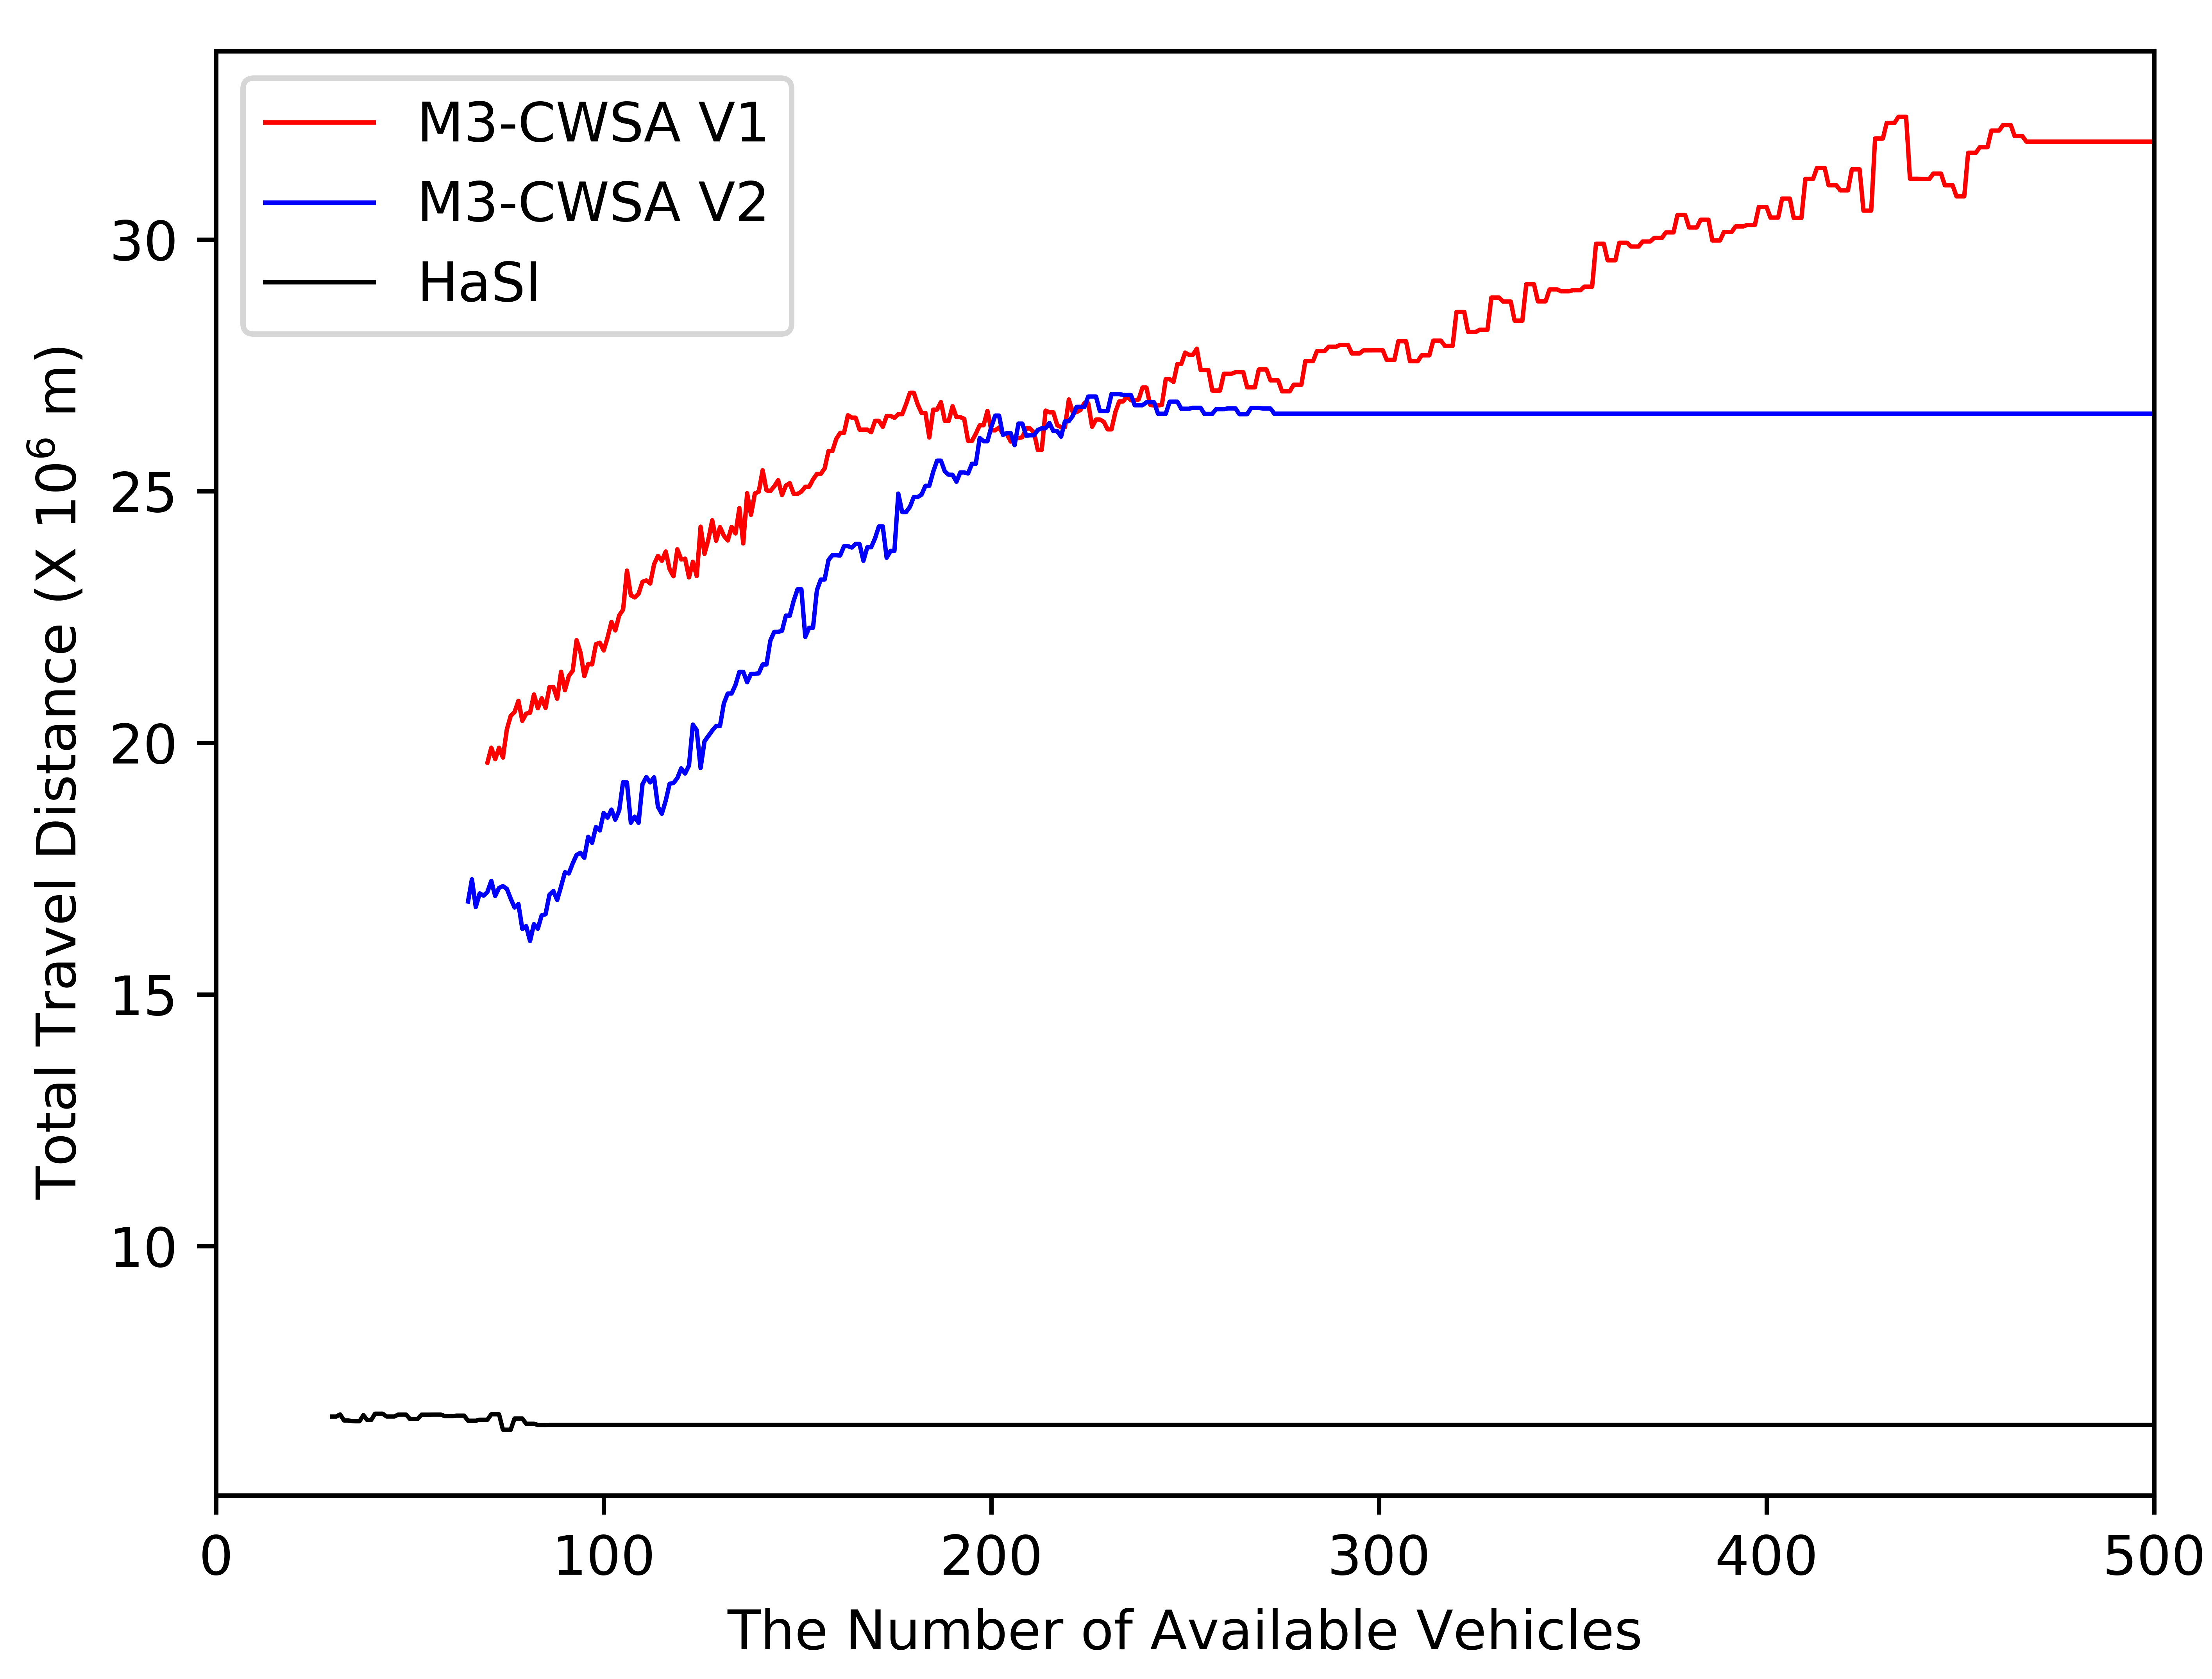
\includegraphics[width=.45\textwidth]{cwsa_dist.png}}
	\end{subfloat}
	\begin{subfloat}[\label{vehicle_cwsa}
			The actual number of occupied vehicles in feasible solutions in Figure~\ref{dist_cwsa}.]{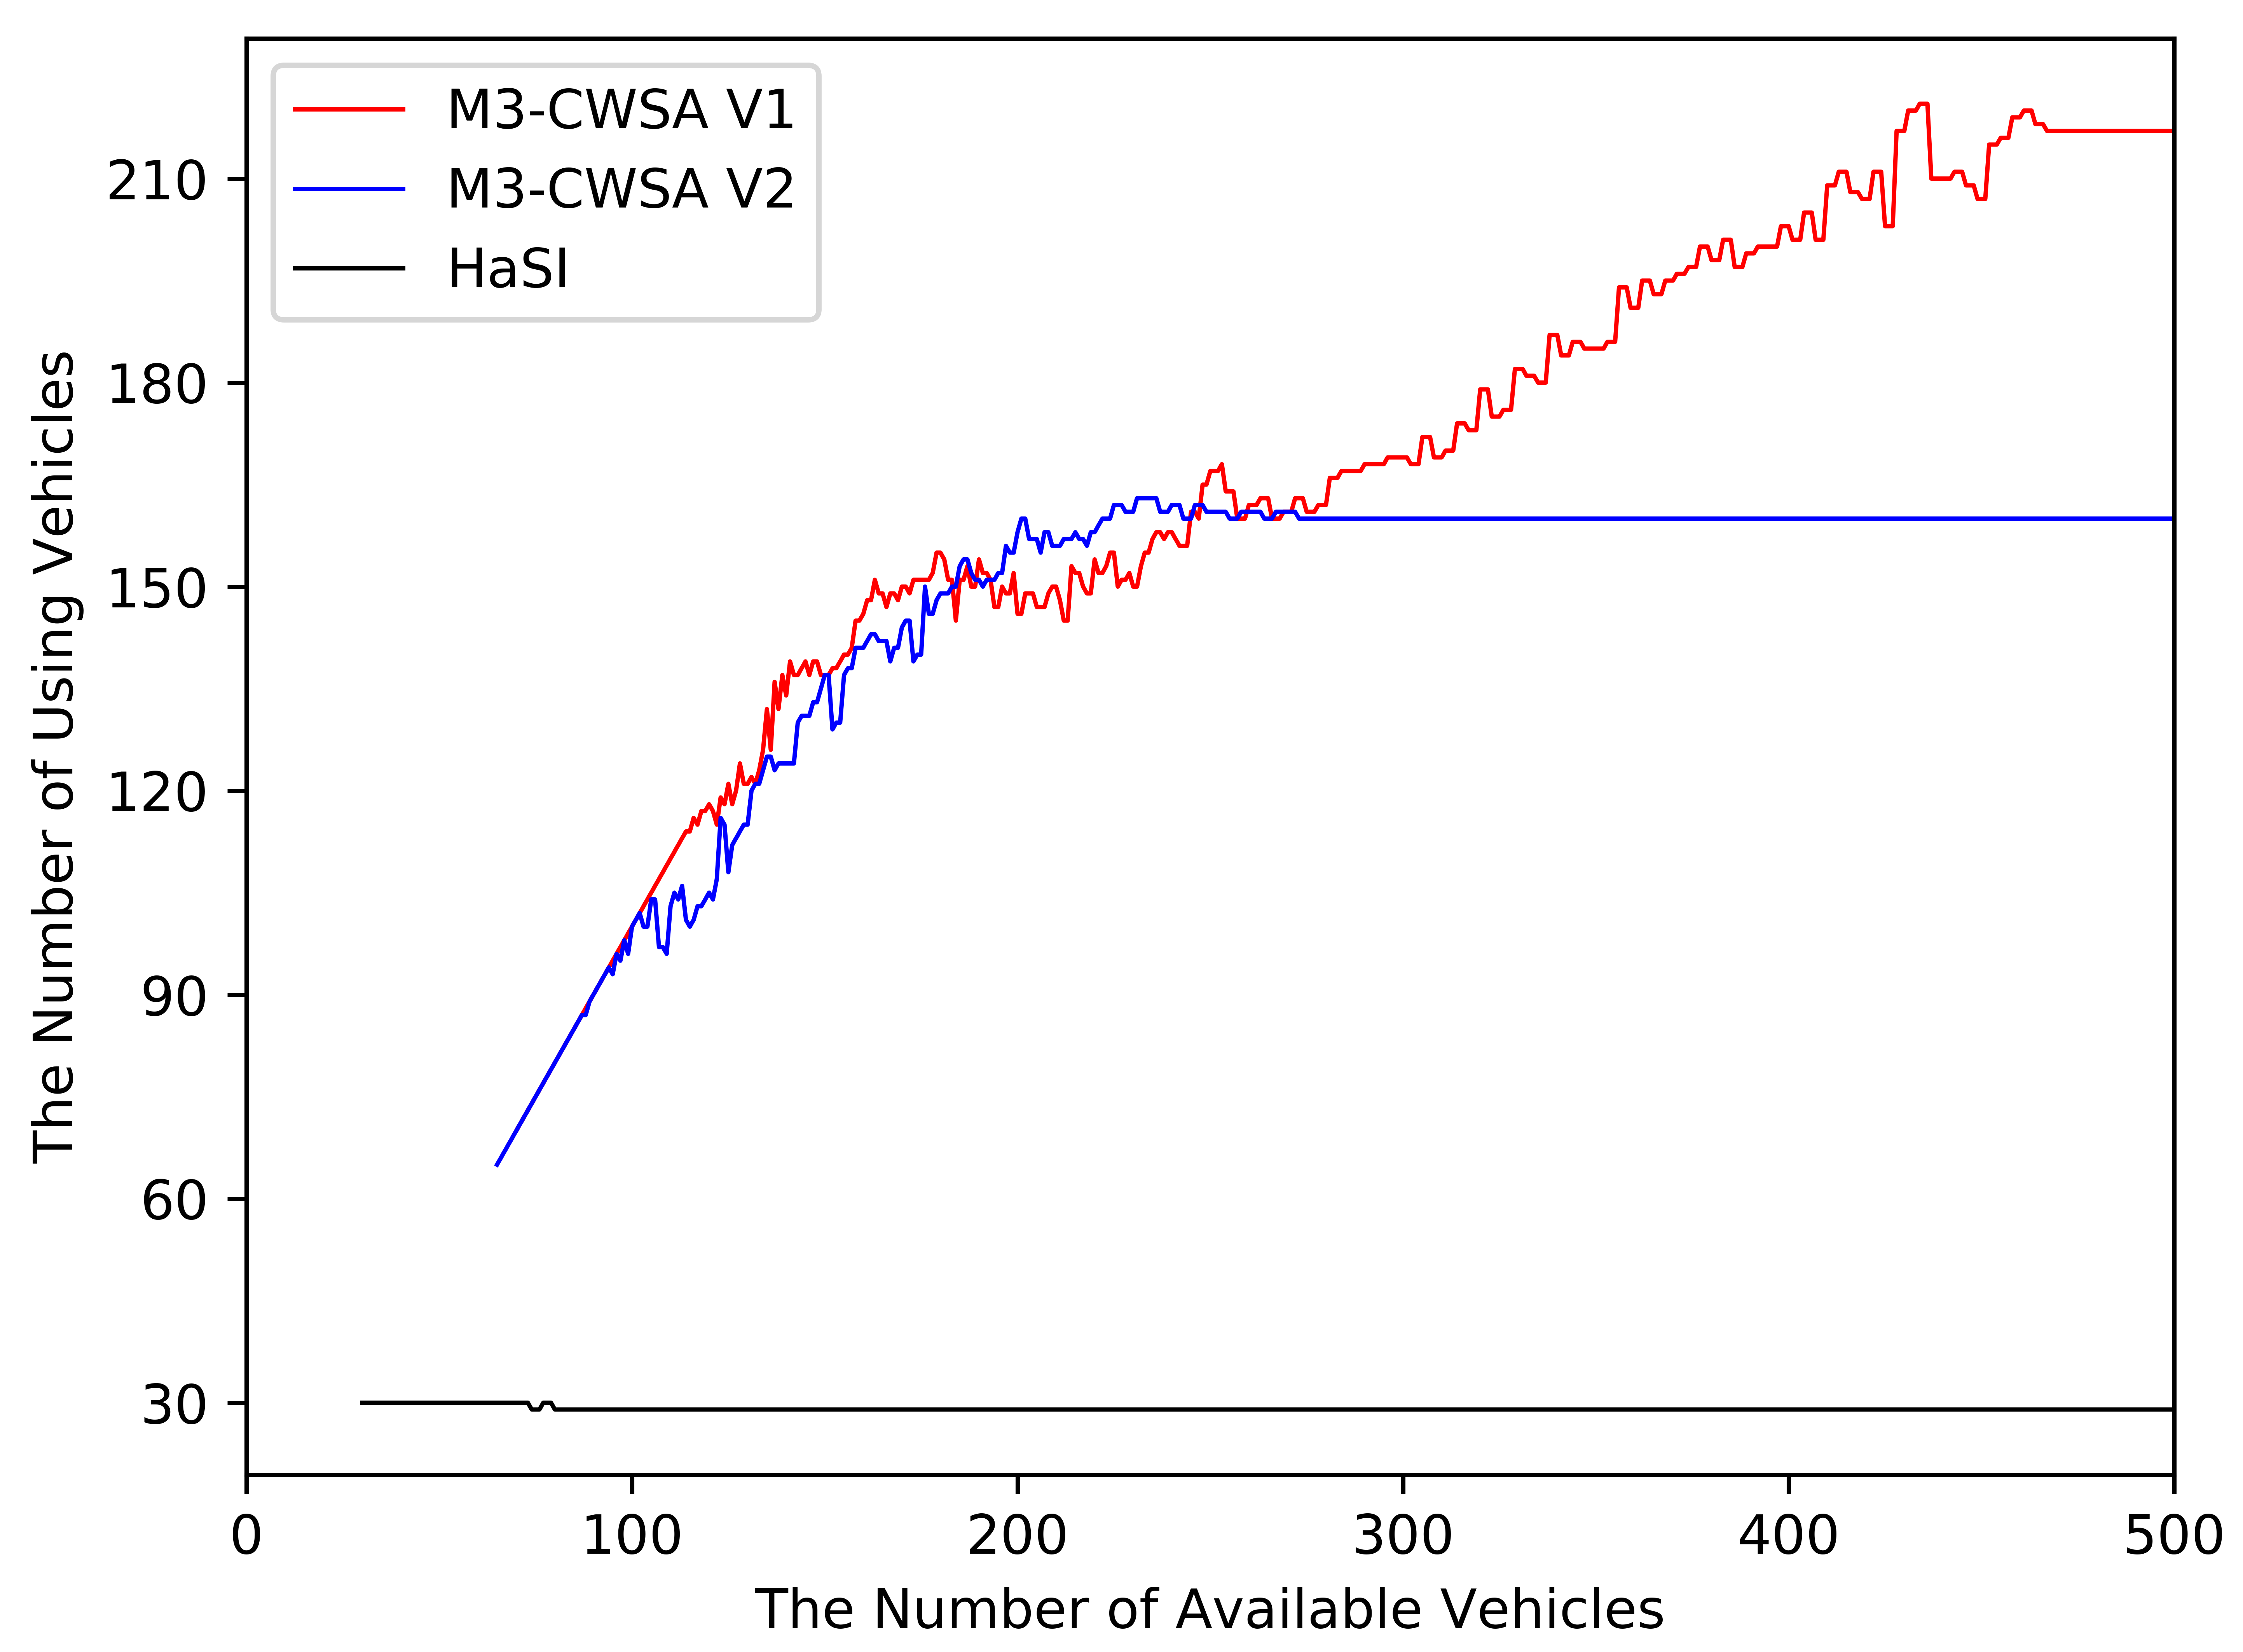
\includegraphics[width=.45\textwidth]{cwsa_vehicle.png}}
	\end{subfloat}
	\caption{\label{init_solution_figure}
	The experimental results of HaSI and M3CWSAs with different $N_{AV}$. Note that when the initial solution construction algorithm cannot generate feasible solution with the given $N_{AV}$, there is no point in illustrating the curve with that $N_{AV}$.}
\end{figure}

According to Figure~\ref{init_solution_figure}, we observe that:
\begin{itemize}%[leftmargin=*,label=(\roman*)]
	\item \label{init_ca} The quality of the feasible solution, including total travel distance and the actual number of occupied vehicles, generated by HaSI is always higher than the one generated by M3CWSAs. Moreover, the quality of the most feasible solutions generated by M3CWSA-\uppercase\expandafter{\romannumeral2} is higher than the one obtained by M3CWSA-\uppercase\expandafter{\romannumeral1}.
	
	\item \label{init_cb} HaSI can find a feasible solution with the minimal number of actually occupied vehicles, followed by M3CWSA-\uppercase\expandafter{\romannumeral1} and M3CWSA- \uppercase\expandafter{\romannumeral2}.
	
	\item \label{init_cc} The total travel distance and the actual number of occupied vehicles in the feasible solutions generated by M3CWSAs both vibrate up and down but showing an overall upward trend as the number of available vehicles increases, and peaking at a specific number. M3CWSAs easily allocate some unserved collection sites to unoccupied vehicles rather than the vehicles which have been occupied but can still load wastes. Since adding a link between unserved site and served site needs to satisfy some stricter constraints than adding a link between two unserved sites. The number of occupied vehicles increases implies that the number of trips from and to the depots increases. Consequently, the total travel distance increases.
	\item \label{init_cd} The total travel distance and the actual number of occupied vehicles of the feasible solution generated by HaSI are generally steady even if they fluctuate at the beginning.
	\item  Sometimes the total travel distance and the actual number of occupied vehicles of feasible solution decrease as the number of available vehicles increases in the local curve. The number of occupied vehicles in $P_1$ decreases if the number of occupied vehicles (available vehicles) in $P_2$ increases since there are more waste collection sites which are closed to $P_2$ as shown in Table~\ref{tab:m3_cwsav2}.
\end{itemize}

% \noindent\textbf{The reason for observation \ref{init_cc}} M3CWSAs easily allocate some unserved waste collection sites to unoccupied vehicles rather than the vehicles which have been occupied but can still load waste since adding a link between unserved collection site and served collection site needs to satisfy some stricter constraints than adding a link between two unserved collection sites, and the number of occupied vehicles increases implies that the number of trips from and to the depots increases. Consequently, the total travel distance increases.

% \noindent\textbf{The reason for observation \ref{init_ce}} The number of occupied vehicles in $P1$ decreases if the number of occupied vehicles (available vehicles) in $P2$ increases since there are more waste collection sites which are closed to $P2$ as Table~\ref{tab:m3_cwsav2} shown.

We highlight some results of Figure~\ref{init_solution_figure} in Table~\ref{tab:initial}. Some closer observation and conclusions which are different from the ones mentioned above can be drawn as follows: \emph{(a)} HaSI and M3CWSAs can generate a feasible solution within a short time. \emph{(b)} The strategy of choosing depot in HaSI still needs to be improved.In summary, HaSI can generate a better feasible solution than M3CWSAs within a shorter computational time in terms of both total travel distance and the number of occupied vehicles.

\begin{table}[htbp]
	\centering
	\caption{\label{tab:m3_cwsav2}
		Highlighted data of feasible solutions generated by M3CWSA-\uppercase\expandafter{\romannumeral2}. $N_V$ and $N_{AV}$ stand for the number of occupied vehicles and available vehicles, respectively. $N_{V_i}$ and $N_{AV_i}$ where $i \in \{1, 2, 3\}$ stand for the number of occupied vehicles and available vehicles in depot $P_i$, respectively. $RT$ stands for the running time of the algorithm.}
	\setlength{\tabcolsep}{1.5pt}
	\begin{tabular}{|c|c|c|ccc|ccc|c|}
		\hline
		$N_{AV}$ & Distance ($m$) & $N_V$ & $N_{AV_1}$ & $N_{AV_2}$ & $N_{AV_3}$ & $N_{V_1}$ & $N_{V_2}$ & $N_{V_3}$ & $RT$ ($s$)\\
		\hline
		100 & 18,606,502 & 100 & 34 & 33 & 33 & 34 & 33 & 33 & 13 \\
		101 & 18,512,327 & 101 & 34 & 34 & 33 & 34 & 34 & 33 & 13 \\
		102 & 18,673,434 & 102 & 34 & 34 & 34 & 34 & 34 & 34 & 13 \\
		103 & 18,471,922 & 100 & 35 & 34 & 34 & 32 & 34 & 34 & 14 \\
		104 & 18,656,519 & 100 & 35 & 35 & 34 & 31 & 35 & 34 & 13 \\
		105 & 19,221,185 & 104 & 35 & 35 & 35 & 34 & 35 & 35 & 13 \\
		106 & 19,212,108 & 104 & 36 & 35 & 35 & 34 & 35 & 35 & 13 \\
		107 & 18,410,268 & 97 & 36 & 36 & 35 & 26 & 36 & 35 & 13 \\
		108 & 18,533,181 & 97 & 36 & 36 & 36 & 25 & 36 & 36 & 13 \\
		109 & 18,410,024 & 96 & 37 & 36 & 36 & 24 & 36 & 36 & 13 \\
		110 & 19,176,613 & 103 & 37 & 37 & 36 & 30 & 37 & 36 & 13 \\
		\hline
	\end{tabular}
\end{table}

\begin{table}[htbp]
	\centering
	\caption{\label{tab:initial}
		Best and worst feasible solutions generated by HaSI and M3CWSAs. $N_V$ and $N_{AV}$ stand for the number of occupied vehicles and available vehicles, respectively. $RT$ stands for the running time of the algorithm.
	}
	\setlength{\tabcolsep}{5pt}
	\begin{tabular}{|c|cccc|}
		\hline
		& Distance ($m$)  & $N_{AV}$ & $N_{V}$ & $RT$ ($s$)\\
		\hline
		Best of HaSI & 6,347,320 & 74 & 29 & $<1$ \\
		Best of M3CWSA-\uppercase\expandafter{\romannumeral1} & 19,606,422  & 70 & 70 & 18 \\
		Best of M3CWSA-\uppercase\expandafter{\romannumeral2} & 1,6059,066 & 81 & 81 & 17\\
		\hline
		Worst of HaSI & 6,664,799 & 43 & 30 & $<1$ \\
		Worst of M3CWSA-\uppercase\expandafter{\romannumeral1} & 32,441,847 & $434 \sim 436$ & 221 & 13 \\
		Worst of M3CWSA-\uppercase\expandafter{\romannumeral2} & 26,929,955 & $232 \sim 233$ & 163 & 12\\
		\hline
	\end{tabular}
\end{table}


\subsubsection{Fine-tuned HaSI}\label{sec:result_hasi}
To get a better feasible solution, HaSI has been fine-tuned by varying the value of $\theta_c$ and $\theta_t$ where $\theta_c \in \{0, 1, \dots, 9, 10\}$ and $\theta_t \in \{0, 1, \dots, 19, 20\}$. In real-world applications, waste collection and transportation company should allocate the available vehicles based on the demand when the total number of the available vehicle is constant. The number of the available vehicle is set as $90$ since $30$ vehicles is enough for each depot.

We observe in Figure~\ref{fig:dist_data_hasi} that most of the feasible solutions generated by HaSI with different values of $\theta_c$ and $\theta_t$ perform well. However, there also exists some feasible solutions with poor performance. The total travel distance of the feasible solution is sensitive to the value of $\theta_c$. The proper value for $\theta_c$ and $\theta_t$ are desirable to select in $\{1, 2,\dots,7\}$ and $\{0, 1,\dots,12\}$ , respectively. The results show that making the actual load of the vehicle as close as possible to the load constraint of the vehicle will not improve the planning result.

\begin{figure}[htbp]
	\centering
	\begin{subfloat}[\label{fig:dist_data_hasi}Total travel distance of the feasible solutions generated by HaSI with different values of $\theta_c$ and $\theta_t$.]{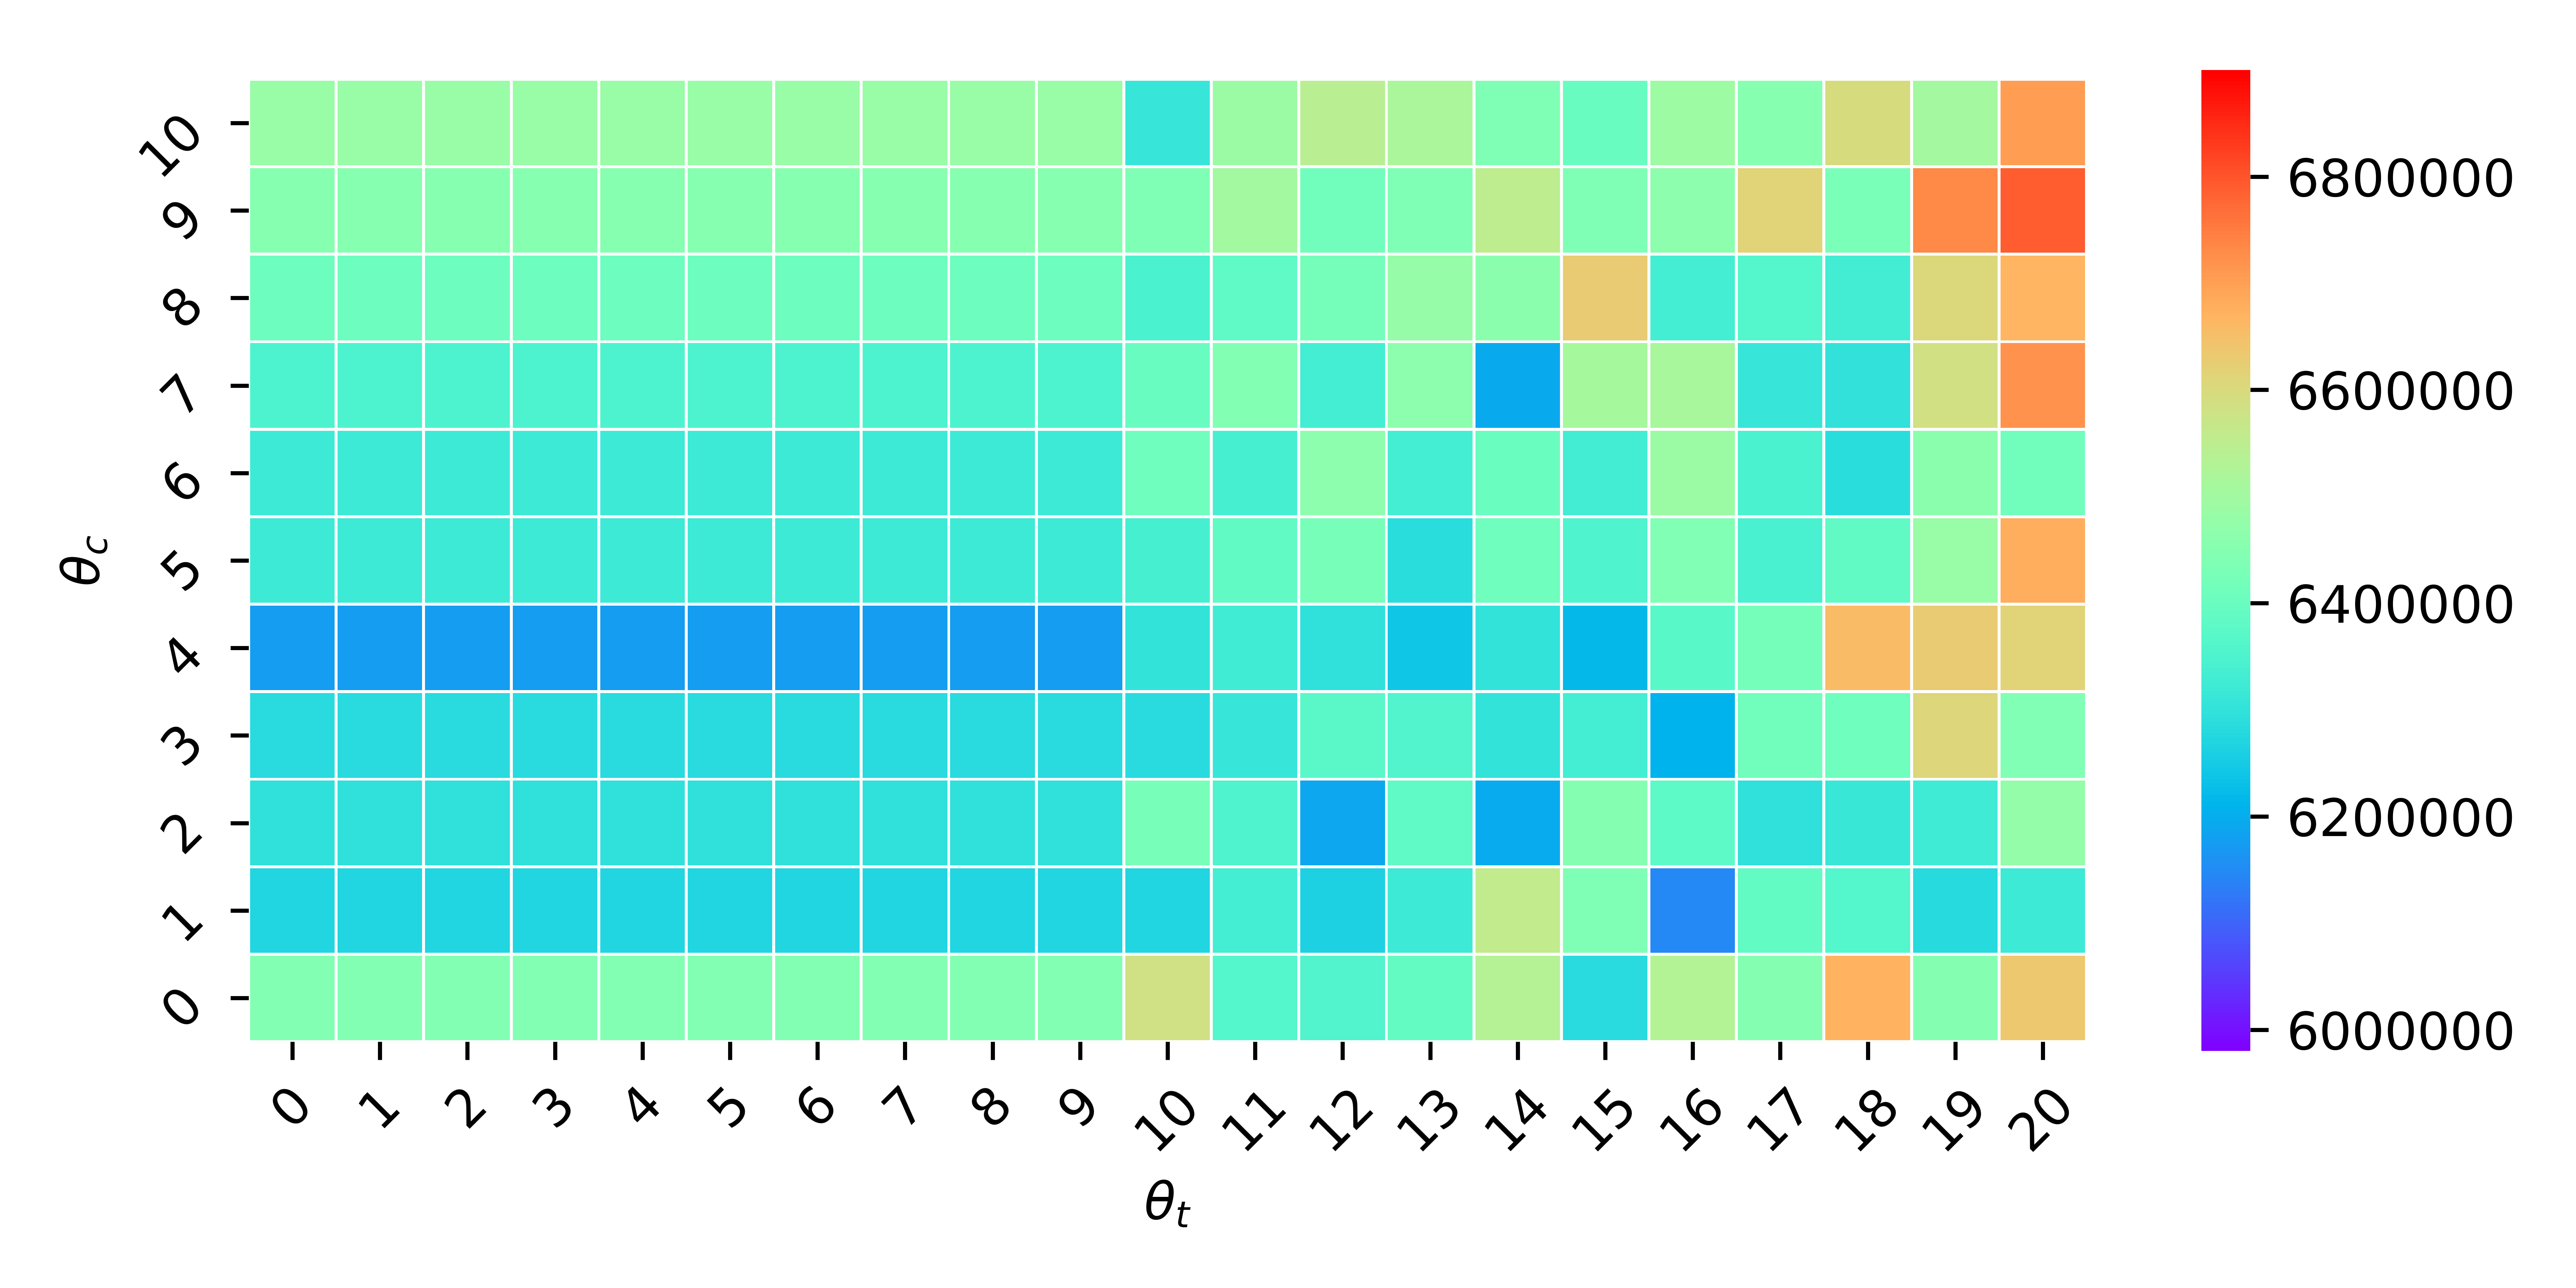
\includegraphics[width=.45\textwidth]{dist_data.png}}
	\end{subfloat}\\\hfill
	\begin{subfloat}[\label{fig:dist_data_bsim} 
			Total travel distance of feasible solutions, in Figure~\ref{fig:dist_data_hasi}, optimised by BSIM.]{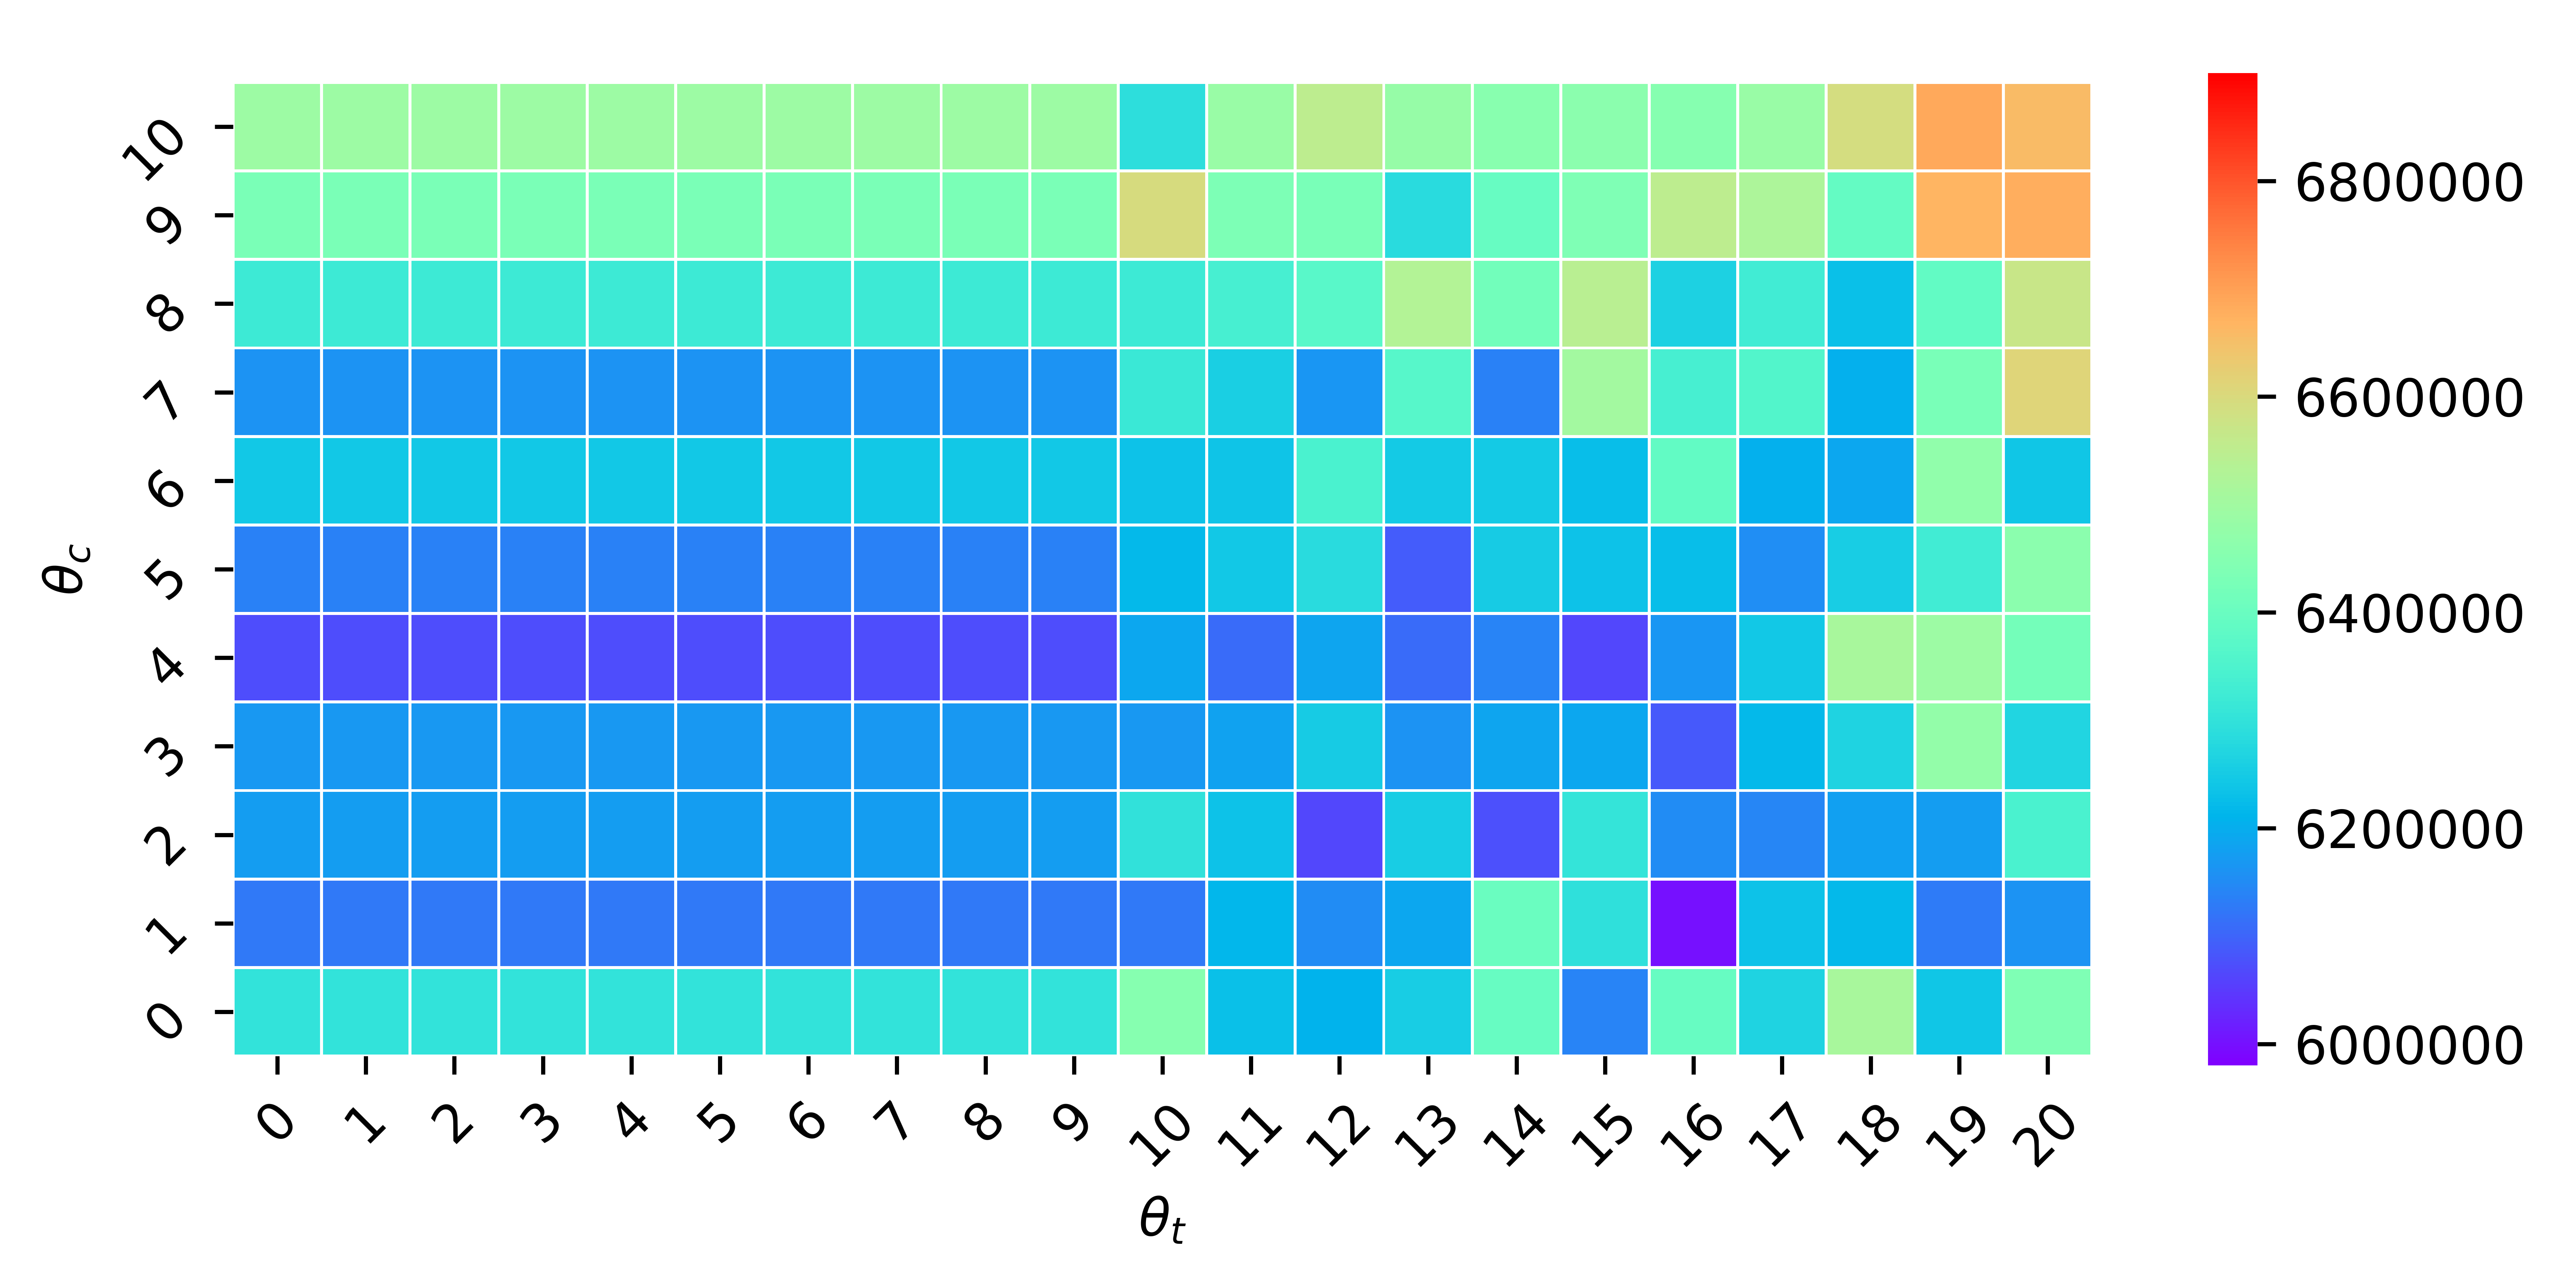
\includegraphics[width=.45\textwidth]{dist_data_bsim.png}}
	\end{subfloat}
	\caption{\label{fig:fine_tuned_hasi}
		Experimental results of the feasible solutions generated by HaSI after fine-tuning (\ref{fig:dist_data_hasi}) and being further optimised by BSIM (\ref{fig:dist_data_bsim}).}
\end{figure}


\subsection{Discussion}\label{sec:init_discuss}
It is surprising that there is a huge difference between the performance of HaSI and M3CWSAs. Some possible reasons are concluded as follows:
\begin{itemize}%[leftmargin=*,label=$Reason_\arabic*$]
	\item \label{reason_1} M3CWSAs have their own obvious disadvantages, shown in Table~\ref{tab:m3_cwsas_pc}.
	\item \label{reason_3} For complex problems, likes M3CVRP, a simple solution solving strategy may be more effective. The \emph{closest-server-first} of HaSI is simpler than the savings formula of M3CWSAs.
	\item \label{reason_4} The initial solution provided by CWSA without any improvement is far from the optimal one~\cite{pichpibul2012an}.
	\item \label{reason_2} CWSA may not be suitable to M3CVRP since not only there are more constraints, but also the distance between any two sites is asymmetrical in M3CVRP.
\end{itemize}

With the purpose of verifying the last reason, we compare the performance of CWSA and HaSI on a \emph{Beigium} dataset\footnote{Available at \url{http://vrp.atd-lab.inf.puc-rio.br/index.php/en/}} with single-depot, no-disposal-facility, single-trip problem instances~\cite{arnold2019efficiently}. For HaSI, $\theta_c$ is set as $0$ since $\theta_c$ only has little influence on single-trip planning, and $\theta_t$ does not exist since there is no working time constraint in this dataset. The distance between any two sites is defined as the Euclidean distance. Table~\ref{tab:beigium} shows the experimental results. The data in column ``CWSA'' are directly obtained from~\cite{arnold2019efficiently}. According to Table~\ref{tab:beigium}, the solutions initialised by CWSA are better than the ones by HaSI on all instances which implicitly proves our hypothesis.
% The runtime of algorithms cannot be compared due to different programming language.
\begin{table}[htbp]
	\centering
	\caption{\label{tab:beigium}
		CWSA v.s. HaSI on \emph{Beigium} dataset. The values in the column with header ``difference'' are obtained by subtracting the values in the ``Distance'' column of HaSI from the values in the ``Distance'' column of CWSA. $RT$ stands for the running time of the algorithm.
	}
	\setlength{\tabcolsep}{5pt}
	\begin{tabular}{|c|cc|cc|c|}
		\hline
		\multirow{2}{*}{Instance ($N$)} & \multicolumn{2}{c|}{CWSA} & \multicolumn{2}{c|}{HaSI} & \multirow{2}{*}{Difference}\\
		& Distance & $RT$ (s) &  Distance & $RT$ (s) & \\
		\hline
		L1(3,000) & 200,957 & 6 & 212,601 & $<1$ & +11,644 \\
		L2(4,000) & 126,122 & 6 & 133,812& 1  & +7,690 \\
		A1(6,000) & 497,441 & 12 & 524,027 & 1 & +26,586\\
		A2(7,000) & 322,073 & 12 & 338,530 & 1 & +16,457 \\
		G1(10,000) & 489,556 & 24 & 507,408 & 2 & +17,852 \\
		G2(11,000) & 288,942 & 24 & 299,775 & 2 & +10,833\\
		B1(15,000) & 531,980 & 36 & 556,691 & 4 & +24,711 \\
		B2(16,000) & 384,437 & 66 & 402,622 & 4 & +18,185 \\
		F1(20,000) & 7,518,845 & 102 & 7,719,804 & 8 & +200,959\\
		F2(30,000) & 4,803,502 & 228 & 4,991,603 & 17 & +188,101 \\
		\hline
	\end{tabular}
\end{table}

\section{Optimisation Methods}\label{sec:optimisation_mathod}
In this section, we first present the solution representation and evaluation function in Section~\ref{sec:sre}. Then, a novel inner-site insertion method is given in Section~\ref{sec:bsim}, and the characteristics of the solution representation determine the necessity of its existence. Afterwards, two proposed optimisation methods are introduced, namely ELS (Section~\ref{sec:els}) and Memetic Algorithm with ELS (MAELS) (Section~\ref{sec:maels}). Finally, the experimental results and discussion are shown in Section~\ref{sec:om_es} and~\ref{sec:om_disscussion}, respectively.

\subsection{Solution Representation and Evaluation}\label{sec:sre}

\subsubsection{Representation} 
Our individuals are represented as permutations of the $V_c$ tasks, without depots and disposal facilities, as in \cite{wang2015estimation}. Consequently, the depots and disposal facilities in the solutions generated by HaSI need to be deleted. When evaluating an individual, the depots and disposal facilities are inserted for calculating \eqref{eq:cost}. Therefore, an insertion method (detailed in Section~\ref{sec:bsim}), which does not make the solution after inserting depot and disposal facilities worse than the initial one before deleting the depots and disposal facilities, is needed.

\subsubsection{Evaluation function}
Same as in \cite{tang2009memetic}, the function for evaluating solutions is defined as
\begin{equation}\label{eq:eval}
f(S) = Cost(S) + \gamma V(S),
\end{equation}
where $Cost(S)$ is the total travel distance of $S$ calculated with \eqref{eq:cost} and $V(S)$ is the total violation of $S$, calculated as the summation of the violations of all routes in $S$. The coefficient $\gamma$ is calculated as $\frac{Cost(S_{best})}{\mu} (\frac{Cost(S_{best})}{Cost(S)}+\frac{Cost(S)}{\mu}+1)$, where the best-so-far solution is represented as $S_{best}$ and the population size is $\mu$ . More details can be found in~\cite{tang2009memetic}. The population size $\mu$ is set as $1$ in ELS.

\subsection{Backspacing Insertion Method}\label{sec:bsim}

In a real-life situation, it may be optimal for a vehicle to dump in advance rather than keeping collecting until the upper bound of load constraint is met. The backspacing insertion method (BSIM) is proposed on account of such kind of situation.

The key of BSIM is described as follows. Firstly, given a route $R_k$ for a vehicle $k$, BSIM will find the latest collection site (indexed by $\tau$) in the first trip that a vehicle can serve before being fulfilled. Afterwards, BSIM will loop over and record all the cases of inserting the closest disposal facility from $(\tau-m)^{th}$ to $\tau^{th}$ collection site, where $m \in \{0, 1, \dots, N_{b}\}$. The next step will start from the latest collection site of next trip and repeat the preceding two steps for generating each trip in route $R_k$. When BSIM reaches the last trip of route $R_k$, the distance $D_{d} = dist({d, c_{k,1,j}})+dist({c_{k,l_k, h_{k,i}}, df})+dist({df, d})$ is calculated for each $d \in V_P$, where $df$ represents the last disposal facility in $R_k$. Then, the depot with the shortest $D_{d}$ is chosen to be the depot of $R_k$. Finally, the route $R_k$'s total distances of all possible combination of cases from the record are calculated, and the best disposal facility insertion plan is selected as the final result.

\subsection{Extended Local Search}\label{sec:els}
By designing 3 novel search operators that are more suitable for M3CVRP, we have extended the local search algorithm as shown in Algorithm~\ref{local}. $\rho_1$, $\rho_2$, $\rho_3$ and $\alpha$ are control parameters.

\subsubsection{Region-constrained single-point swap (RCSPS)}
For each collection site $c$ in a randomly selected route $R_k$ from a given solution $S$, if there exists at least one site in other routes that locate within a certain distance $\rho_1$, then a site is randomly picked up. Let $c'$ denote the selected site, and $R_{k'}$ is its corresponding route. Two new routes, $R_k^{'}$ and $R_{k'}^{'}$, can be obtained after switching $c$ and $c'$. If the inequality $C_r(R_k^{'})+C_r(R_{k'}^{'})<C_r(R_k)+C_r(R_{k'})$ 
holds, then this swap operation will be accepted; otherwise, nothing will happen.

\subsubsection{Region-constrained segment swap (RCSS)} 
For a given solution $S$, a waste collection site $c$ is randomly selected from a route $R_k$ selected uniformly at random. If there exists at least one site in other routes that locate within a certain distance $\rho_2$, then randomly choose one $c'$ from route $R_{k'}$ among all alternatives. The two new routes, $R_k^{'}$ and $R_{k'}^{'}$, can be obtained after swapping the whole segments after $c$ and $c'$. If $C_r(R_k^{'})+C_r(R_{k'}^{'})<C_r(R_k)+C_r(R_{k'})$, then the swap operation is accepted; otherwise, nothing will happen.

\subsubsection{Relaxed multi-point swap (RMPS)} 
For a given solution $S$, two routes $R_1$ and $R_2$ are randomly selected. A small proportion are randomly selected from each route, denoted as $B_1$ and $B_2$. Two new routes $R_1'$ and $R_2'$ are generated by randomly inserting the sites of $B_2$ into $R_1$ and the sites of $B_1$ into $R_2$ with the best position, respectively. The best position is the one where the lowest cost (calculated with (\ref{eq:cost})) is achieved, and the insertion order of sites in $B_1$ and $B_2$ is random. If $C_r(R'_{1})+C_r(R'_{2}) \leq C_r(R_1)+C_r(R_2)+\rho_3$, $R_1$ and $R_2$ are replaced by $R'_1$ and $R'_2$, respectively. $C_r(R)$ is the total travel distance of a route $R$, detailed previously in Section~\ref{sec:m3cvrp}.

\subsubsection{Insertion} 
Arbitrarily select a waste collection site $c$ from a randomly selected route $R_k$ in a given solution $S$, and then re-insert $c$ into the best position of $R_k$ to obtain a new route $R_{k}^{'}$. The definition of the best position is the same as the best position mentioned in RMPS. If $C_r(R_{k}^{'})<C_r(R_k)$, then the insertion operation is accepted; otherwise, no operation occurs.

\subsubsection{Swap} In the swap search operator, two waste collection sites are randomly selected from a randomly selected route $R_k$, and then their positions are exchanged to obtain a new route $R_{k}^{'}$. Similarly, if $C_r(R_{k}^{'})<C_r(R_k)$, then the swap operation is accepted; otherwise, no operation occurs.

\subsubsection{2-opt} Two kinds of 2-opt search operators exist, one for a single route and the other for double routes~\cite{tang2009memetic}. Only the operator for a single route is employed in ELS since region-constrained segment swap has similar search operation as the 2-opt for double routes. In the 2-opt operator for a single route, two waste collection sites $c_1$ and $c_2$ are randomly selected from a randomly selected route $R_k$, and then a new route $R_{k}^{'}$ is obtained after revering the visiting order of the waste collection sites between $c_1$ and $c_2$. Similarly, if $C_r(R_{k}^{'})<C_r(R_k)$, then this type of reverse operation is accepted; otherwise, no operation occurs.

Our extended local search (ELS) applies the above novel search operators together with three classic search operators, \emph{insertion}, \emph{swap} and \emph{2-opt}~\cite{BeullensA}, in an order defined in Algorithm~\ref{local}, to improve input solutions. 

The main idea of designing RCSPS and RCSS are as follows: \emph{(a)} Reducing search space with its ``region-constrained'' since the search space for large-scale M3CVRP is huge. \emph{(b)} Increasing search step size for being capable of searching within a broader neighbourhood since those three classic search operators have small search step size such that they can only search within a small neighbourhood~\cite{tang2009memetic}. The purpose of RMPS is to help other search operators jump out of the local optimum with its ``relaxation'' of $\rho_3$.

\begin{figure}[htbp]
		\centering
		\begin{tikzpicture}
			\draw (0.5,0) circle (1.5);
			\draw (-1,0)--(0.5,0);
			\fill[blue] (0.5,0) circle (0.1);
			\fill[red] (1,0) circle (0.1);
			\fill[red] (2,0) circle (0.1);
			\fill[red] (1.4,0.8) circle (0.1);
			\fill[red] (-0.5,-0.8) circle (0.1);
			\fill[red] (1.5,-0.7) circle (0.1);
			\draw (-0.25, 0.2) node {$\rho_1$};
			\draw (0.65, -0.15) node {$c$};
			\draw (1.55,0.65) node {$k$};
			
			\draw (5,0) circle (1.5);
			\draw (3.5,0)--(5,0);
			\fill[blue] (5,0) circle (0.1);
			\fill[red] (5.5,0) circle (0.1);
			\fill[red] (6.5,0) circle (0.1);
			\fill[red] (5.9,0.8) circle (0.1);
			\fill[red] (4,-0.8) circle (0.1);
			\fill[red] (6,-0.7) circle (0.1);
			\draw (4.25, 0.2) node {$\rho_2$};
			\draw (5.15, -0.15) node {$c$};
			\draw (6.05,0.65) node {$k$};
			
		\end{tikzpicture}
		\begin{tikzpicture}
			\draw (-5,0) node {$Route\ A: a\rightarrow b\rightarrow c\rightarrow d \rightarrow e \rightarrow f$};
			\draw (-5,-0.5) node {$Route\ B: h\rightarrow i\rightarrow j\rightarrow k \rightarrow l \rightarrow m \rightarrow n$};
		\end{tikzpicture}
		\caption{\label{fig:novel_operator}
			Demonstration of search operators RCSPS (\emph{left}) and RCSS (\emph{right}), assuming two routes $A$ and $B$. If the swap condition is valid, RCSPS will replace $A$ and $B$ will by $a\rightarrow b\rightarrow k\rightarrow d \rightarrow e \rightarrow f$ and $ h \rightarrow i\rightarrow j\rightarrow c \rightarrow l \rightarrow m \rightarrow n$, respectively, while RCSS will change $A$ and $B$ to $a\rightarrow b\rightarrow k\rightarrow l \rightarrow m \rightarrow n$ and $ h \rightarrow i\rightarrow j\rightarrow c \rightarrow d \rightarrow e \rightarrow f$, respectively.
		}
	\end{figure}

\begin{algorithm}[htbp]
	\caption{\label{local}ELS, proposed by us in Section \ref{sec:els}. Stopping criteria $SC_1$ and $SC_2$ are user-defined.}
	{\bf Input:}
	A original solution $S$; control parameters $\rho_1$, $\rho_2$, $\rho_3$ and $\alpha$
	%\hspace*{0.02in} 
	%{\bf Output:} New solution $S'$ %and corresponding vector of depots and vector of facilities
	\begin{algorithmic}[1]
		%\State Delete the depots and disposal facilities in the $S_0$\rpj{delete this line};
		%\State Set current solution $S = S_0$, best solution $S_b = S$;
		\State $S' \leftarrow S$
		\While{stopping criterion $SC_1$ not met}
		\While{stopping criterion $SC_2$ not met}
		\State \rpj{Apply RCSPS with parameter $\rho_1$ on $S'$}
		\State \rpj{Apply RCSS with parameter $\rho_2$ on $S'$}
		\State \rpj{Apply swap, insertion and 2-opt operators \emph{each once in a random order} on $S'$}
		%\If{$dist(S) <  dist(S_b)$}
		%    \State $S_b$ = $S$;
		%\EndIf
		\EndWhile
		\State \rpj{Apply RMPS with parameters $\rho_3$ and $\alpha$ on $S'$}
		\EndWhile
		\State \Return $S'$
	\end{algorithmic}
\end{algorithm}

%In Algorithm~\ref{local}, the initial solution $S_0$ is the best solution $S_b$ selected from the population $P$ created by Algorithm 1, where $S_b$ is the solution with minimal total distance. 
%\lwx{In order to make the mutation more convenient for optimisation later, we have deleted all disposal facilities $V_P$ and starting and ending parking lots $V_D$ in the route (line 1).} 
%\todo{why can delete? RPJ:I don't think it is necessary to say we delete the depots and disposal facility as we already show how we represent the solution in~\ref{sec:model}, and this is just a trick to make algorithm easier to be implemented.} 
\subsection{Memetic Algorithm with ELS (MAELS)}\label{sec:maels}


The Memetic Algorithm (MA) was introduced by Moscato in 1989~\cite{moscato1989evolution}. Comparing to GA, the mutation operators of GA are replaced by local search in MA, which is the main difference between MA and GA~\cite{tang2009memetic}. Consequently, MA can balance well between generality and problem specificity due to the domain-specific heuristics embedded in local search operators~\cite{tang2009memetic}. In this paper, we integrate ELS to an MA~\cite{moscato1989evolution,tang2009memetic}. The details of our MA with ELS (MAELS) are given in Algorithm~\ref{algo:ma}. 
%REPEATED SETENCE:It is important for MA to have an initial population with high diversity since low diversity of the population is the reason which is often mentioned when an evolutionary algorithm has poor performance~\cite{yuan2008research}.
It is important for MA to have an initial population with high diversity. 
%Consequently, a measure of population diversity is needed. 
The difference among the solutions in a population is the set of collection sites allocated to the same vehicle and the traversal order among these sites. The trip is the smallest set of sites in a population. Moreover, we do not consider the traversal order of sites in trips since exact methods can found the optimal order. Consequently, we measure the diversity of the initialised population~\cite{maekawa1997genetic} using the an entropy defined as 
\begin{equation}\label{eq:diversity}
H = \mathbf{-}\sum_{trip \in T} \Gamma_{trip} \log{\Gamma_{trip}},
\end{equation} 
where $\Gamma_{trip}=\frac{n_{trip}}{\mu}$ and $n_{trip}=\sum_{i=1}^{\mu} \mathbf{1}(trip \in T_i)$. $T_i$ denotes the set of trips appeared in solution $S_i$, $\forall i \in \{1,\dots, \mu\}$. $T$ is the set of all trips appeared in the population, i.e., $T=\cup_{i=1}^{\mu}T_i$. For all $i \in \{1,\dots, \mu\}$, $\mathbf{1}(trip \in T_i)=1$ if $trip \in T_i$ is true; otherwise, $\mathbf{1}(trip \in T_i)=0$.


\begin{algorithm}[htbp]
	\caption{\label{algo:ma}MAELS, proposed by us in Section \ref{sec:maels}. SBX refers to a sequence-based crossover operator~\cite{potvin1996vehicle}.}
	{\bf Input:} an initial population $P$ of size $\mu$, a maximum number of offspring $\lambda$, and $p_{ELS}$, the probability of applying ELS
	\begin{algorithmic}[1]
		\While{time not elapsed}
		\State offspring$\leftarrow \emptyset$
		%\State Set an intermediate population $P'$ = $P$
		\For{$i = 1,2,\dots,\lambda$ }
		\State Randomly select two distinct solutions $S_1$ and $S_2$ from $P$ as parents
		\State Apply the SBX operator to $S_1$ and $S_2$ to generate two new solutions, then evaluate and keep the one with shorter distance as $S'$
		% \State Sample a random number $r$ from the uniform distribution between 0 and 1
		\If{ $UniformRandom(0,1)<p_{ELS}$}
		\State $S'' \leftarrow$ Apply ELS to $S'$
		\If{$S''$ is not a clone of any solution in offspring or $P$}
		\State Add $S''$ to offspring
		%offspring = offspring \cup \{S''\}$;
		\ElsIf{$S'$  is not a clone of any solution in offspring or $P$}
		\State Add $S'$ to offspring
		%\State $offspring = offspring \cup \{S'\}$;
		\EndIf
		\ElsIf{$S'$ is not a clone of any solution in offspring or $P$}
		\State Add $S'$ to offspring
		%\State $offspring = offspring \cup \{S'\}$;
		\EndIf
		\EndFor
		%\State Evaluate individuals in $offspring$
		\State Sort the solutions in $P \cup$ offspring using stochastic ranking \cite{runarsson2000stochastic}
		\State Set $P$ = \{the best $\mu$ individuals in $P \cup$ offspring\}
		\EndWhile
		\State\Return the best feasible solution in $P$
	\end{algorithmic}
\end{algorithm}


\subsection{Experimental Study}\label{sec:om_es}

With the intention of better evaluating the BSIM, novel search operators, ELS and MAELS, three sets of experiments have been carried out. In the first set, we use BSIM to insert disposal facilities and depots into solutions, i.e., permutations of waste collection sites (Section~\ref{sec:eff_bsim}). After that, we comprehensively compare the effectiveness and contribution of each novel operator in ELS in Section~\ref{sec:ls_els}. A comparison of optimisation effect between ELS and MAELS is performed on the last set (Section~\ref{sec:els_maels}). Besides, we preliminary verify the validity of the diversity measure described in Section~\ref{sec:els_maels}.

%\lwx{Both programming language and program running time environment in this section are same as the Section~\ref{sec:initial_solution}}.

\subsubsection{Effectiveness of BSIM}\label{sec:eff_bsim}
To verify the effectiveness of BSIM, we optimised the feasible solutions generated by HaSI, the quality of which are demonstrated in Figure~\ref{fig:dist_data_hasi}. First, the depots and disposal facilities in those solutions are deleted. Then, BSIM inserts the depots and disposal facilities in its way. The optimisation results are shown in Figure~\ref{fig:dist_data_bsim} with the control parameter $N_b$=$5$. By comparing Figures~\ref{fig:dist_data_bsim} and~\ref{fig:dist_data_hasi}, we can conclude that BSIM can optimise the feasible solutions generated with $\theta_c\in \{0,1,\dots,8\}$ and cannot optimise part of the feasible solutions generated with $\theta_c\in \{9,10\}$. The reason is that the load of vehicle $k$ is impossible to reach the level of $0.9* Capacity(k)$ or $0.91* Capacity(k)$ when $N_b$ is set as 5.

%In conclusion, BSIM will not make solutions after deleting depot and disposal facilities worse than the solution before deleting depot and disposal facilities as long as $N_b$ is large enough.

In conclusion, BSIM has the probability to optimise the solutions and will not make solutions worse by re-inserting depots and disposal facilities as long as $N_b$ is large enough.
%\todo[inline]{Should we explicitly state RQ (research questions)?}

\subsubsection{LS v.s. ELS}\label{sec:ls_els}
\begin{table*}[htbp]
	\centering
	\caption{\label{tab:ls_els_comparison}
		The comparison between ELS, LS and LS with different single novel search operator. ``BEST'' and ``AVG'' stand for the best and average distances obtained from 30 independent runs. ``STD'' stands for the standard deviation. The lowest average distance is marked with *. Results in bold (or underline) indicate that the corresponding algorithm is better (or worse) than LS based on Wilcoxon rank-sum test with the level of significance $0.05$.}
	\setlength{\tabcolsep}{1.4pt}
	\scriptsize
	\begin{tabular}{|c|ccc|ccc|ccc|ccc|ccc|ccc|ccc|ccc|}
		\hline
		\multirow{1}{*}{Time} & 
		\multicolumn{3}{c|}{LS} &
		\multicolumn{3}{c|}{LS+RCSPS} &
		\multicolumn{3}{c|}{LS+RCSS} &
		\multicolumn{3}{c|}{LS+RMPS} &
		\multicolumn{3}{c|}{LS+RCSPS+RMPS} &
		\multicolumn{3}{c|}{LS+RCSS+RMPS} &
		\multicolumn{3}{c|}{LS+RCSPS+RCSS} &
		\multicolumn{3}{c|}{ELS}\\
		
		(mins)& BEST & AVG & STD & BEST & AVG & STD & BEST & AVG & STD & BEST & AVG & STD & BEST & AVG & STD & BEST & AVG & STD& BEST & AVG & STD& BEST & AVG & STD \\
		\hline
		0 & 6148.0 & 6148.0 & 0.0 & 6148.0 & 6148.0 & 0.0 & 6148.0 & 6148.0 & 0.0 & 6148.0 & 6148.0 & 0.0 & 6148.0 & 6148.0 & 0.0 & 6148.0 & 6148.0 & 0.0 & 6148.0 & 6148.0 & 0.0 & 6148.0 & 6148.0 & 0.0 \\
		0.5 & 5844.9 & 5853.1 & 4.7 & 5781.5 & \textbf{5801.6} & 14.9 & 5692.4 & \textbf{5758.8} & 20.4 & 5819.6 & 5848.2 & 12.7 & 5776.7 & \textbf{5796.9} & 11.5 & 5715.3 & \textbf{5752.8} & 16.1 & 5719.0 & \textbf{5748.6}* & 16.2 & 5719.2 & \textbf{5761.3} & 20.7 \\
		1 & 5843.9 & 5852.4 & 4.6 & 5771.7 & \textbf{5786.3} & 9.8 & 5664.5 & \textbf{5740.0} & 25.8 & 5815.5 & \textbf{5843.4} & 13.4 & 5767.6 & \textbf{5784.6} & 8.0 & 5694.1 & \textbf{5734.5} & 18.3 & 5688.7 & \textbf{5719.5}* & 14.5 & 5695.5 & \textbf{5727.7} & 15.6 \\
		1.5 & 5843.2 & 5852.3 & 4.7 & 5769.5 & \textbf{5781.7} & 7.7 & 5651.4 & \textbf{5731.3} & 26.2 & 5809.2 & \textbf{5837.1} & 16.1 & 5743.5 & \textbf{5780.5} & 10.2 & 5683.1 & \textbf{5725.6} & 20.2 & 5674.4 & \textbf{5704.4}* & 13.6 & 5686.7 & \textbf{5713.2} & 16.8 \\
		2 & 5843.2 & 5852.3 & 4.7 & 5768.7 & \textbf{5779.9} & 7.7 & 5650.6 & \textbf{5726.0} & 26.6 & 5808.6 & \textbf{5832.1} & 15.4 & 5739.0 & \textbf{5777.9} & 10.6 & 5681.0 & \textbf{5719.3} & 21.6 & 5668.0 & \textbf{5695.6}* & 14.5 & 5680.8 & \textbf{5704.8} & 17.3 \\
		2.5 & 5843.2 & 5852.3 & 4.7 & 5767.7 & \textbf{5778.8} & 7.4 & 5650.6 & \textbf{5722.9} & 26.4 & 5808.0 & \textbf{5831.0} & 14.7 & 5737.4 & \textbf{5774.1} & 13.0 & 5680.4 & \textbf{5716.0} & 22.1 & 5662.1 & \textbf{5690.7}* & 14.4 & 5673.1 & \textbf{5698.6} & 17.4 \\
		3 & 5843.2 & 5852.3 & 4.7 & 5766.1 & \textbf{5778.2} & 7.6 & 5648.6 & \textbf{5719.6} & 26.3 & 5808.0 & \textbf{5828.4} & 12.8 & 5733.2 & \textbf{5772.6} & 13.8 & 5674.0 & \textbf{5714.2} & 23.4 & 5660.5 & \textbf{5687.2}* & 15.0 & 5668.7 & \textbf{5692.8} & 16.9 \\
		6 & 5843.2 & 5852.3 & 4.7 & 5764.6 & \textbf{5776.7} & 7.7 & 5646.8 & \textbf{5712.5} & 27.4 & 5803.0 & \textbf{5825.2} & 13.1 & 5732.9 & \textbf{5762.1} & 16.8 & 5645.8 & \textbf{5707.9} & 26.5 & 5631.7 & \textbf{5675.3} & 16.0 & 5641.1 & \textbf{5675.1}* & 15.7 \\
		9 & 5843.2 & 5852.3 & 4.7 & 5764.6 & \textbf{5776.4} & 7.7 & 5646.8 & \textbf{5710.8} & 27.5 & 5803.0 & \textbf{5824.1} & 13.1 & 5732.6 & \textbf{5757.9} & 16.2 & 5644.8 & \textbf{5706.9} & 25.8 & 5619.5 & \textbf{5668.7} & 17.0 & 5618.4 & \textbf{5665.7}* & 19.2 \\
		12 & 5843.2 & 5852.3 & 4.7 & 5764.4 & \textbf{5776.3} & 7.7 & 5646.8 & \textbf{5710.4} & 27.8 & 5801.6 & \textbf{5823.0} & 12.5 & 5731.1 & \textbf{5754.9} & 14.1 & 5644.8 & \textbf{5705.2} & 26.4 & 5619.5 & \textbf{5664.0} & 17.9 & 5613.1 & \textbf{5660.7}* & 19.0 \\
		15 & 5843.2 & 5852.3 & 4.7 & 5764.4 & \textbf{5776.3} & 7.8 & 5646.8 & \textbf{5710.4} & 27.8 & 5801.6 & \textbf{5822.4} & 12.5 & 5731.1 & \textbf{5752.0} & 12.5 & 5644.8 & \textbf{5704.0} & 26.8 & 5619.4 & \textbf{5661.3} & 19.2 & 5605.7 & \textbf{5656.9}* & 19.9 \\
		30 & 5843.2 & 5852.3 & 4.7 & 5764.4 & \textbf{5776.2} & 7.7 & 5646.8 & \textbf{5710.4} & 27.8 & 5801.6 & \textbf{5819.1} & 12.7 & 5724.5 & \textbf{5749.3} & 11.8 & 5644.8 & \textbf{5698.5} & 26.9 & 5618.2 & \textbf{5657.9} & 20.0 & 5601.7 & \textbf{5649.3}* & 20.6 \\
		45 & 5843.2 & 5852.3 & 4.7 & 5764.4 & \textbf{5776.2} & 7.7 & 5646.8 & \textbf{5710.4} & 27.8 & 5798.9 & \textbf{5816.9} & 12.7 & 5724.5 & \textbf{5747.1} & 10.4 & 5643.8 & \textbf{5693.2} & 28.5 & 5618.2 & \textbf{5657.2} & 20.0 & 5601.5 & \textbf{5645.9}* & 21.3 \\
		60 & 5843.2 & 5852.3 & 4.7 & 5764.4 & \textbf{5776.2} & 7.7 & 5646.8 & \textbf{5710.4} & 27.8 & 5796.1 & \textbf{5814.4} & 12.6 & 5724.5 & \textbf{5746.3} & 9.7 & 5624.8 & \textbf{5686.9} & 30.3 & 5618.2 & \textbf{5656.9} & 20.1 & 5601.5 & \textbf{5642.4}* & 21.8 \\
		75 & 5843.2 & 5852.3 & 4.7 & 5764.4 & \textbf{5776.2} & 7.7 & 5646.8 & \textbf{5710.4} & 27.8 & 5796.1 & \textbf{5812.1} & 11.5 & 5724.5 & \textbf{5745.6} & 9.8 & 5624.4 & \textbf{5676.2} & 26.7 & 5618.2 & \textbf{5656.9} & 20.1 & 5601.5 & \textbf{5641.7}* & 22.0 \\
		90 & 5843.2 & 5852.3 & 4.7 & 5764.4 & \textbf{5776.2} & 7.7 & 5646.8 & \textbf{5710.4} & 27.8 & 5794.2 & \textbf{5809.9} & 11.7 & 5722.7 & \textbf{5745.2} & 9.9 & 5624.4 & \textbf{5672.3} & 26.1 & 5618.2 & \textbf{5656.9} & 20.1 & 5601.5 & \textbf{5640.8}* & 22.6 \\
		105 & 5843.2 & 5852.3 & 4.7 & 5764.4 & \textbf{5776.2} & 7.7 & 5646.8 & \textbf{5710.4} & 27.8 & 5783.1 & \textbf{5806.9} & 11.5 & 5722.7 & \textbf{5744.2} & 9.2 & 5613.2 & \textbf{5669.3} & 26.5 & 5618.2 & \textbf{5656.9} & 20.1 & 5601.5 & \textbf{5640.0}* & 22.8 \\
		120 & 5843.2 & 5852.3 & 4.7 & 5764.4 & \textbf{5776.2} & 7.7 & 5646.8 & \textbf{5710.4} & 27.8 & 5783.1 & \textbf{5803.5} & 9.4 & 5722.7 & \textbf{5742.6} & 8.8 & 5610.1 & \textbf{5666.5} & 26.9 & 5618.2 & \textbf{5656.9} & 20.1 & 5599.3 & \textbf{5639.1}* & 22.5 \\
		135 & 5843.2 & 5852.3 & 4.7 & 5764.4 & \textbf{5776.2} & 7.7 & 5646.8 & \textbf{5710.4} & 27.8 & 5775.1 & \textbf{5800.8} & 10.8 & 5719.0 & \textbf{5740.5} & 9.6 & 5569.3 & \textbf{5661.6} & 30.4 & 5618.2 & \textbf{5656.9} & 20.1 & 5597.2 & \textbf{5636.9}* & 20.5 \\
		150 & 5843.2 & 5852.3 & 4.7 & 5764.4 & \textbf{5776.2} & 7.7 & 5646.8 & \textbf{5710.4} & 27.8 & 5775.1 & \textbf{5799.0} & 11.2 & 5712.7 & \textbf{5739.4} & 10.1 & 5565.9 & \textbf{5657.1} & 28.9 & 5618.2 & \textbf{5656.9} & 20.1 & 5583.4 & \textbf{5635.7}* & 21.8 \\
		165 & 5843.2 & 5852.3 & 4.7 & 5764.4 & \textbf{5776.2} & 7.7 & 5646.8 & \textbf{5710.4} & 27.8 & 5774.1 & \textbf{5796.2} & 11.6 & 5711.2 & \textbf{5738.7} & 10.1 & 5563.9 & \textbf{5654.4} & 29.3 & 5618.2 & \textbf{5656.9} & 20.1 & 5569.2 & \textbf{5634.7}* & 23.4 \\
		180 & 5843.2 & 5852.3 & 4.7 & 5764.4 & \textbf{5776.2} & 7.7 & 5646.8 & \textbf{5710.4} & 27.8 & 5773.2 & \textbf{5794.5} & 12.1 & 5711.2 & \textbf{5737.7} & 9.6 & 5563.1 & \textbf{5650.8} & 30.4 & 5618.2 & \textbf{5656.9} & 20.1 & 5568.5 & \textbf{5633.7}* & 23.8 \\
		195 & 5843.2 & 5852.3 & 4.7 & 5764.4 & \textbf{5776.2} & 7.7 & 5646.8 & \textbf{5710.4} & 27.8 & 5772.9 & \textbf{5792.3} & 12.5 & 5711.2 & \textbf{5736.8} & 10.0 & 5561.2 & \textbf{5648.1} & 30.5 & 5618.2 & \textbf{5656.9} & 20.1 & 5568.5 & \textbf{5633.2}* & 24.0 \\
		210 & 5843.2 & 5852.3 & 4.7 & 5764.4 & \textbf{5776.2} & 7.7 & 5646.8 & \textbf{5710.4} & 27.8 & 5772.9 & \textbf{5791.2} & 12.5 & 5711.2 & \textbf{5736.2} & 10.1 & 5561.0 & \textbf{5643.0} & 31.7 & 5618.2 & \textbf{5656.9} & 20.1 & 5568.5 & \textbf{5631.8}* & 24.2 \\
		225 & 5843.2 & 5852.3 & 4.7 & 5764.4 & \textbf{5776.2} & 7.7 & 5646.8 & \textbf{5710.4} & 27.8 & 5772.9 & \textbf{5790.0} & 12.8 & 5693.8 & \textbf{5734.7} & 12.5 & 5561.0 & \textbf{5641.2} & 31.5 & 5618.2 & \textbf{5656.9} & 20.1 & 5568.5 & \textbf{5630.3}* & 24.2 \\
		240 & 5843.2 & 5852.3 & 4.7 & 5764.4 & \textbf{5776.2} & 7.7 & 5646.8 & \textbf{5710.4} & 27.8 & 5763.6 & \textbf{5788.0} & 13.8 & 5693.8 & \textbf{5733.7} & 12.7 & 5561.0 & \textbf{5639.2} & 30.8 & 5618.2 & \textbf{5656.9} & 20.1 & 5568.5 & \textbf{5628.8}* & 22.9 \\
		\hline
	\end{tabular}
\end{table*}

\begin{figure}[htbp]
	\centering
		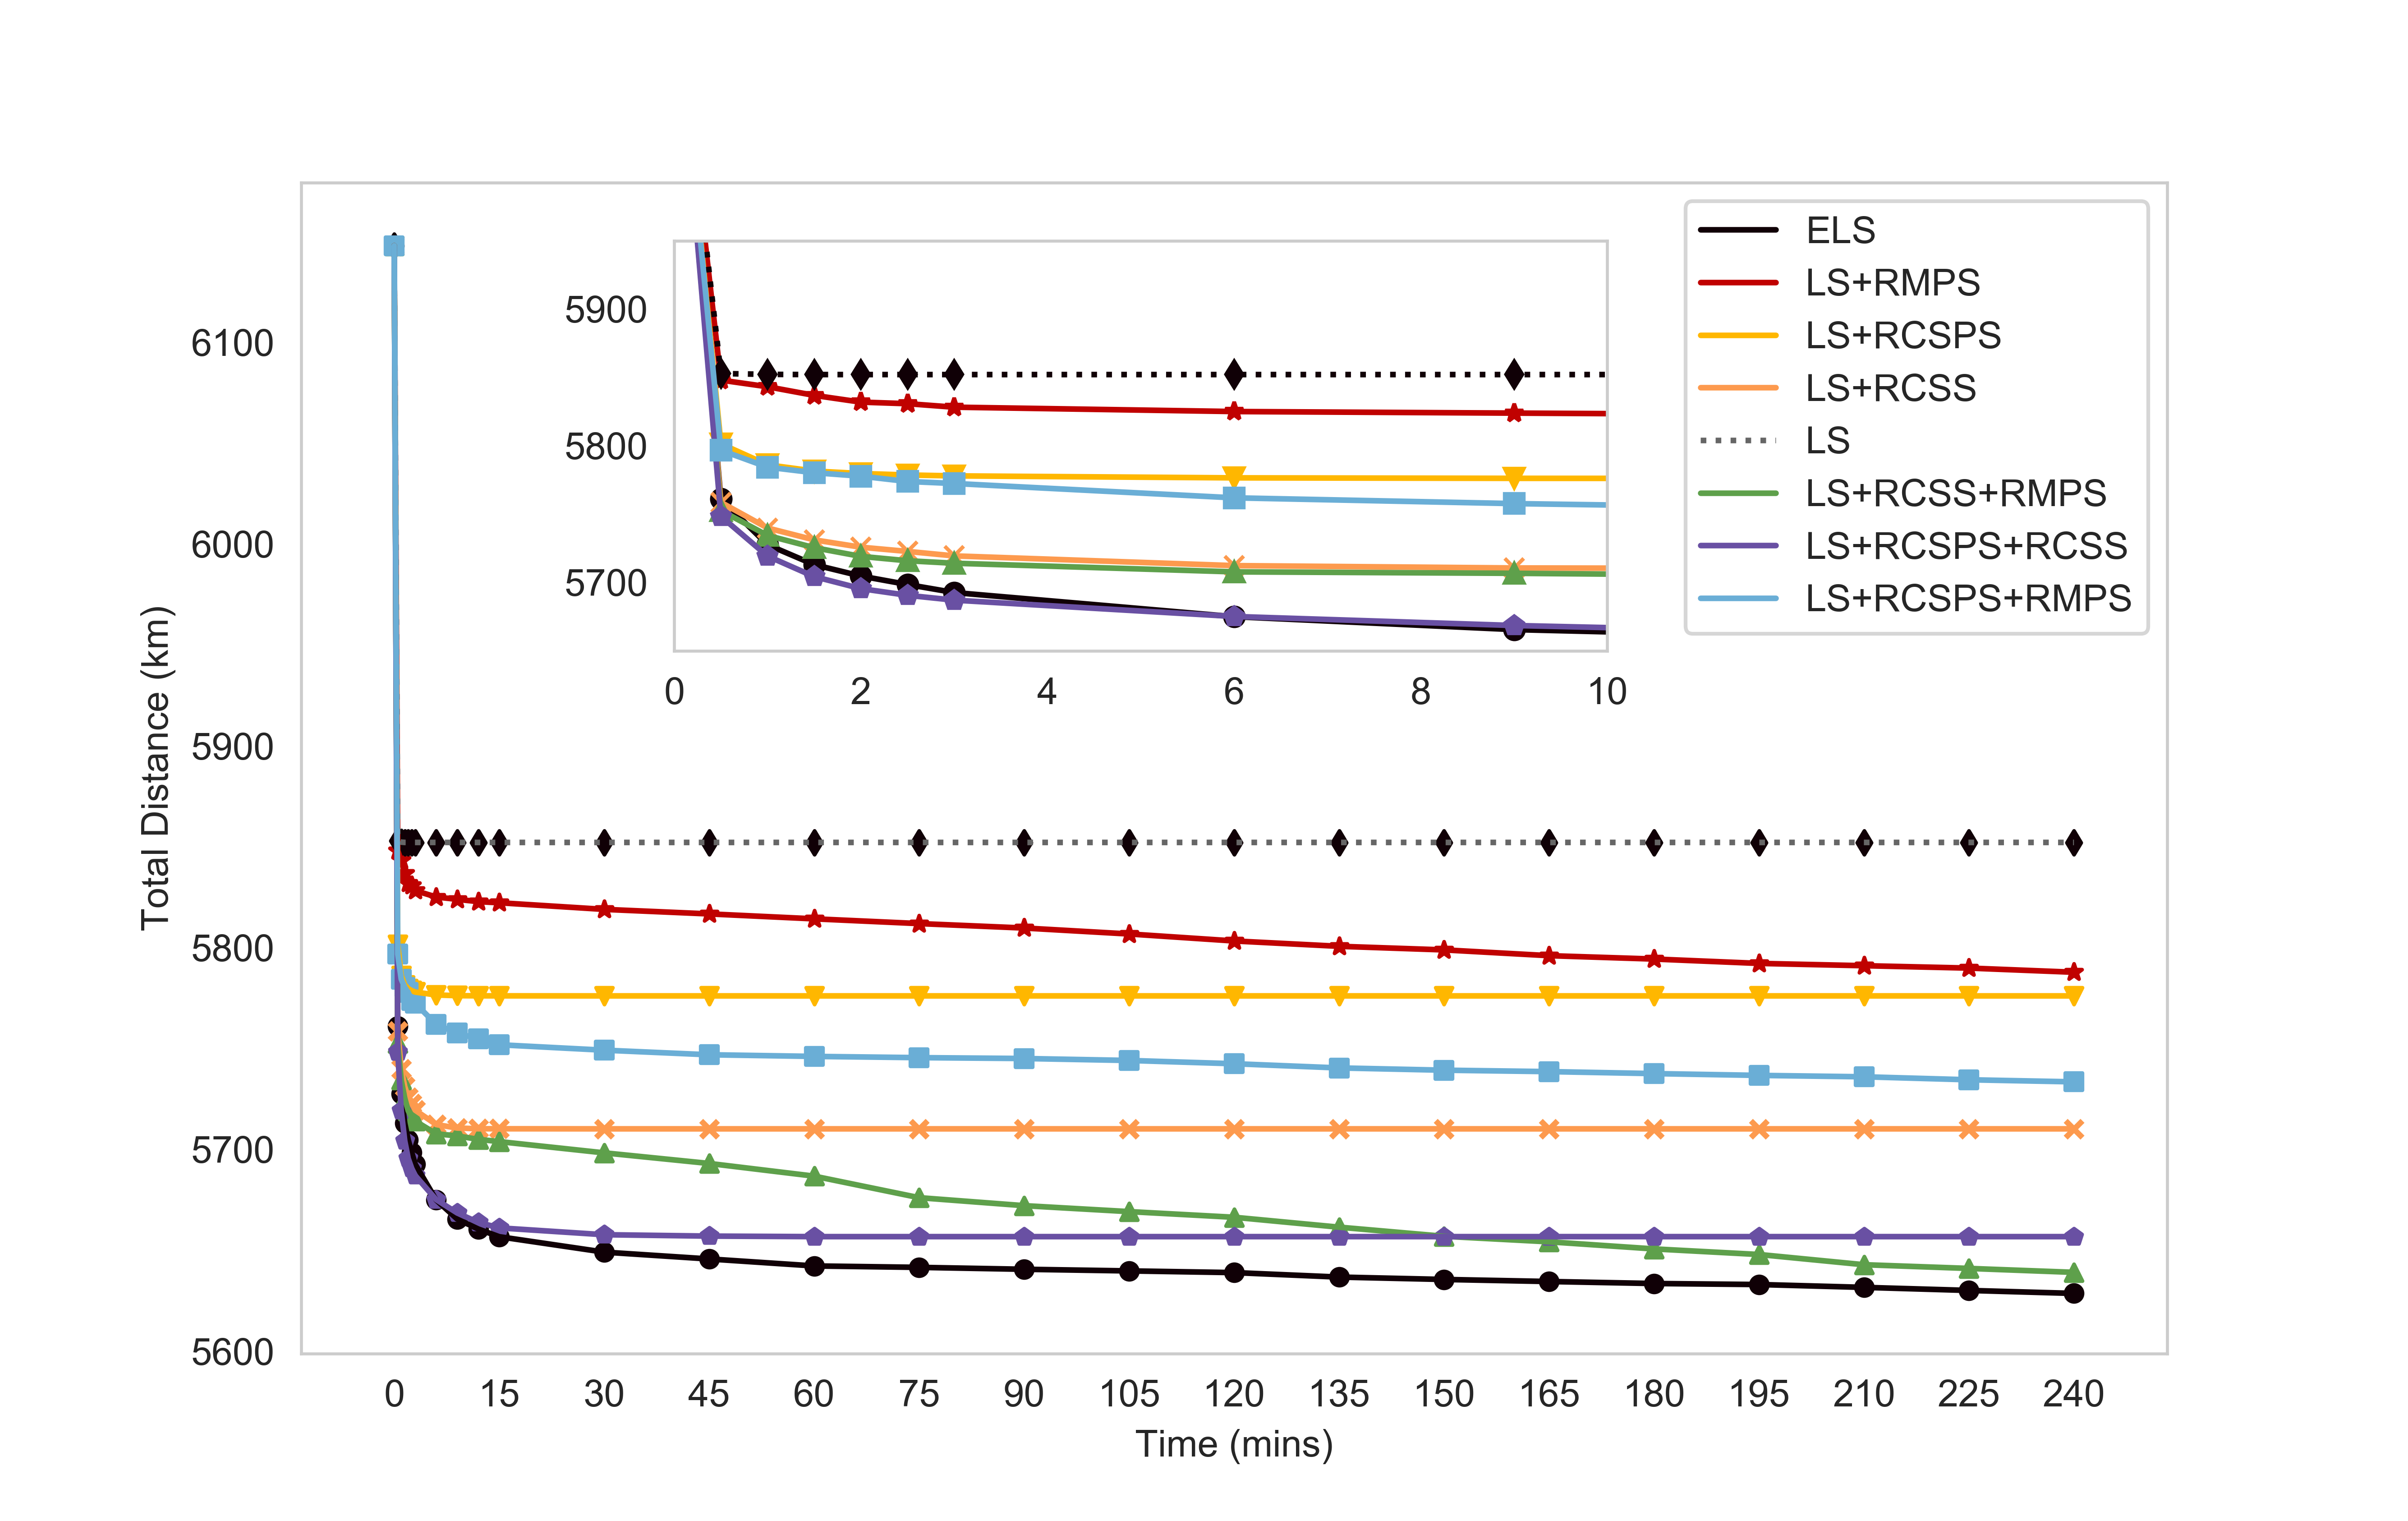
\includegraphics[width=1\columnwidth]{ls_els_more_nostd.png}
	\caption{\label{ls_els_figure}
		Comparison between LS, LS with all combinations of novel search operators and ELS in terms of total travel distance. Table~\ref{tab:ls_els_comparison} presents the corresponding figures and standard deviations.}
\end{figure}

In order to better understand the effectiveness and contribution of each novel search operator in ELS, a comparative experiment has been carried out, and the experimental results are shown in Figure~\ref{ls_els_figure} and Table~\ref{tab:ls_els_comparison}. We compare LS, ELS and different usage combination of the three novel search operators (RMPS, RCSS and RCSPS) to exploit the impact of each operator. The control parameters $\rho_1$ and $\rho_2$ are set as $5km$, and $\rho_3$ is set as $15km$. $\alpha$ is set as $1/|R_k|$ where $R_k$ is randomly picked in RMPS. In other words, only one point will be swapped in RMPS. Additionally, the stopping criteria $SC_1$ and $SC_2$ are if the running time of the program has been exceeded 4 hours and if the reduction of total travel distance does not exceed $2km$ for $5$ consecutive iterations, respectively. This parameter setting is arbitrarily chosen.

Figure~\ref{ls_els_figure} and Table \ref{tab:ls_els_comparison} show that:
\begin{enumerate}[label=(\roman*)]
	\item \label{ob_1} RMPS can help other search operators to jump out of the local optimum, but its step size is relatively small at each generation. Only one point will be swapped in RMPS, which rarely leads to large mutations.
    RMPS relaxes too much would result in skipping the neighbourhood of global optimum. Determining the optimal degree of relaxation for efficient convergence is crucial.
	\item \label{ob_2} Both RCSS and RCSPS can perform efficient searches, but premature convergence occurs. It may be explained by the ``region-constrained'' feature which limits the search space of RCSPS and RCSS and the right search direction driven by heuristics.
	\item \label{ob_3} Within the first few minutes or less, the average distances of solutions optimised by LS variants embedded with RCSS are slightly lower than the ones by ELS (cf. Table \ref{tab:ls_els_comparison}). Since RCSS in ELS has iterated fewer times than LS variants embedded with RCSS within the same time.
	\item \label{ob_4} RCSPS and RCSS have the steadiest and the most unstable optimisation effect among three novel search operators, respectively. For RCSPS, the waste collection site can only be swapped with the ones within a certain distance $\rho_1$. Therefore, the solutions of independent optimisation runs of RCSPS are similar due to the small search space of RCSPS. On the contrary, the optimised solutions by RCSS are quite different since RCSS's search space is larger than the one of RCSPS. The benefit from RCSPS or RCSS in terms of reduced distance by RCSPS or RCSS is limited, but these two operators significantly change the neighbourhood that will be searched by insert, 2-Opt and swap operators.
\end{enumerate}

% \noindent\textbf{Why RMPS has relatively small step size each time:} Only one point will be swapped in RMPS, which rarely leads to large mutations.
%As a result, it is not too possible to has large search step size with this parameter setting for RMPS. 
% RMPS relaxes too much would result in skipping the neighbourhood of global optimum.
%Additionally, it may miss the global optimum if RMPS relaxes too much. 
% Determining the optimal degree of relaxation for efficient convergence is crucial.

% \noindent\textbf{The reason for \ref{ob_2}:} \ref{ob_2} may be explained by the ``region-constrained'' feature which limits the search space of RCSPS and RCSS and the right search direction driven by heuristics.\todo[inline]{check if the above one is better the one below.}
% \lwx{It may be because the "region-constrained" limits the search space of RCSPS and RCSS and direction of search chosen with heuristic is correct. Additionally, both RCSPS and RCSS are meet partial gain criterion is possible the reason why they soon fall into a local optimum.}

% \noindent\textbf{The reason for \ref{ob_3}:} 
% Since RCSS in ELS has iterated fewer times than LS series algorithm with RCSS within the same time.
% \lwx{Since the running iterations of RCSS in ELS is smaller than in LS series algorithm with RCSS within the same time. In other words, there are more search operators needed to be run in ELS than LS series algorithm with RCSS.}

% \noindent\textbf{The reason for \ref{ob_4}:} For RCSPS, the waste collection point can only be swapped with the ones within a certain distance $\rho_1$. Therefore, the solutions of independent optimisation runs of RCSPS are similar due to the small search space of RCSPS. On the contrary, the optimised solutions by RCSS are quite different since RCSS's search space is larger than the one of RCSPS. The benefit from RCSPS or RCSS in terms of reduced distance by RCSPS or RCSS is limited, but these two operators significantly change the neighbourhood that will be searched by insert, 2-Opt and swap operators.

In summary, RMPS mainly helps ELS jump out of the local optimum, and RCSPS not only makes ELS have steady optimisation performance but also help ELS reach a better solution more efficiently. For ELS, on the one hand, RCSS can change a lot the neighbourhood which is then searched by other operators. On the other hand, RCSS can improve the efficiency of ELS.
 
\subsubsection{ELS v.s. MAELS}\label{sec:els_maels}
Three questions are investigated in this subsection: \emph{(RQ1)} Can the MA framework help ELS jump out of the local optimum? \emph{(RQ2)} How much does the MA contribute to the MAELS framework? \emph{(RQ3)} Is the proposed population diversity measure \eqref{eq:diversity} valid? 

For parameter setting, the population size $\mu$ of MAELS/MALS is $30$, and the size of offspring $\lambda$ and the probability of applying ELS/LS in MAELS/MALS $p_{ELS}$ are set as $6\mu$ and 0.2, respectively. All these parameters are set to the same as the parameters in~\cite{tang2009memetic}. The Figure~\ref{fig:dist_data_hasi} illustrates that the initial population of MAELS/MALS with high (or low) diversity is chosen from the population with highest (or lowest) diversity among $10,000$ populations which are obtained by randomly choosing $30$ feasible solutions from the set of solutions. To make the comparison between ELS and MAELS more comprehensible, the initial population must contain the feasible solution optimised by ELS in the last set of experiment. In other words, there are only $29$ feasible solutions being picked randomly in the initial solutions. Expressly, stopping criteria $SC_1$ of ELS used in MAELS is set as if the number of iterations of that loop has been exceeded 5. The $SC_1$ and $SC_2$ are arbitrarily set.

The experimental results (Table \ref{data_comparison} and Figure~\ref{fig:maels}) illustrate that:
\begin{itemize}%[label=(\roman*)]
	\item \label{ma_ob1}MAELS has better optimisation performance than MALS.
	\item \label{ma_ob2}MAELS/MALS has better optimisation effect to the high diversity initial population than to the low diversity initial population.
	\item \label{ma_ob3}ELS can obtain better solutions than MAELS\_High (i.e., MAELS initialised with a population of high diversity) during the early stage of optimisation. Though, MAELS\_High can get solutions of similar or even better quality than ELS after the optimisation time increased to 135 minutes.
\end{itemize}

In the solutions optimised by MAELS\_High among 30 independent runs, there are few vehicles (the maximum number is $3$) whose working time exceeded 8 hours and up to 20 minutes in some solutions. It is usually acceptable in real applications. Additionally, with a focus on studying the optimisation effect of ELS and MAELS after optimising for a longer time, we perform a supplementary experiment and illustrate the results in Figure~\ref{fig:maels_12}. After three hours' optimisation, there is no significant difference between the optimisation effects of ELS and MAELS.

In conclusion, our novel diversity measurement is sufficient. Moreover, ELS plays an essential role in the optimisation process of MAELS. Although the framework of MA might helps the ELS to jump out of the local optimum, MAELS needs to take more time on optimising.

\begin{figure}[htbp]
	\centering
	\begin{subfloat}[\label{fig:maels}
		MAELS and MALS are initialised with two identical populations of low and high diversity, separately.]{
	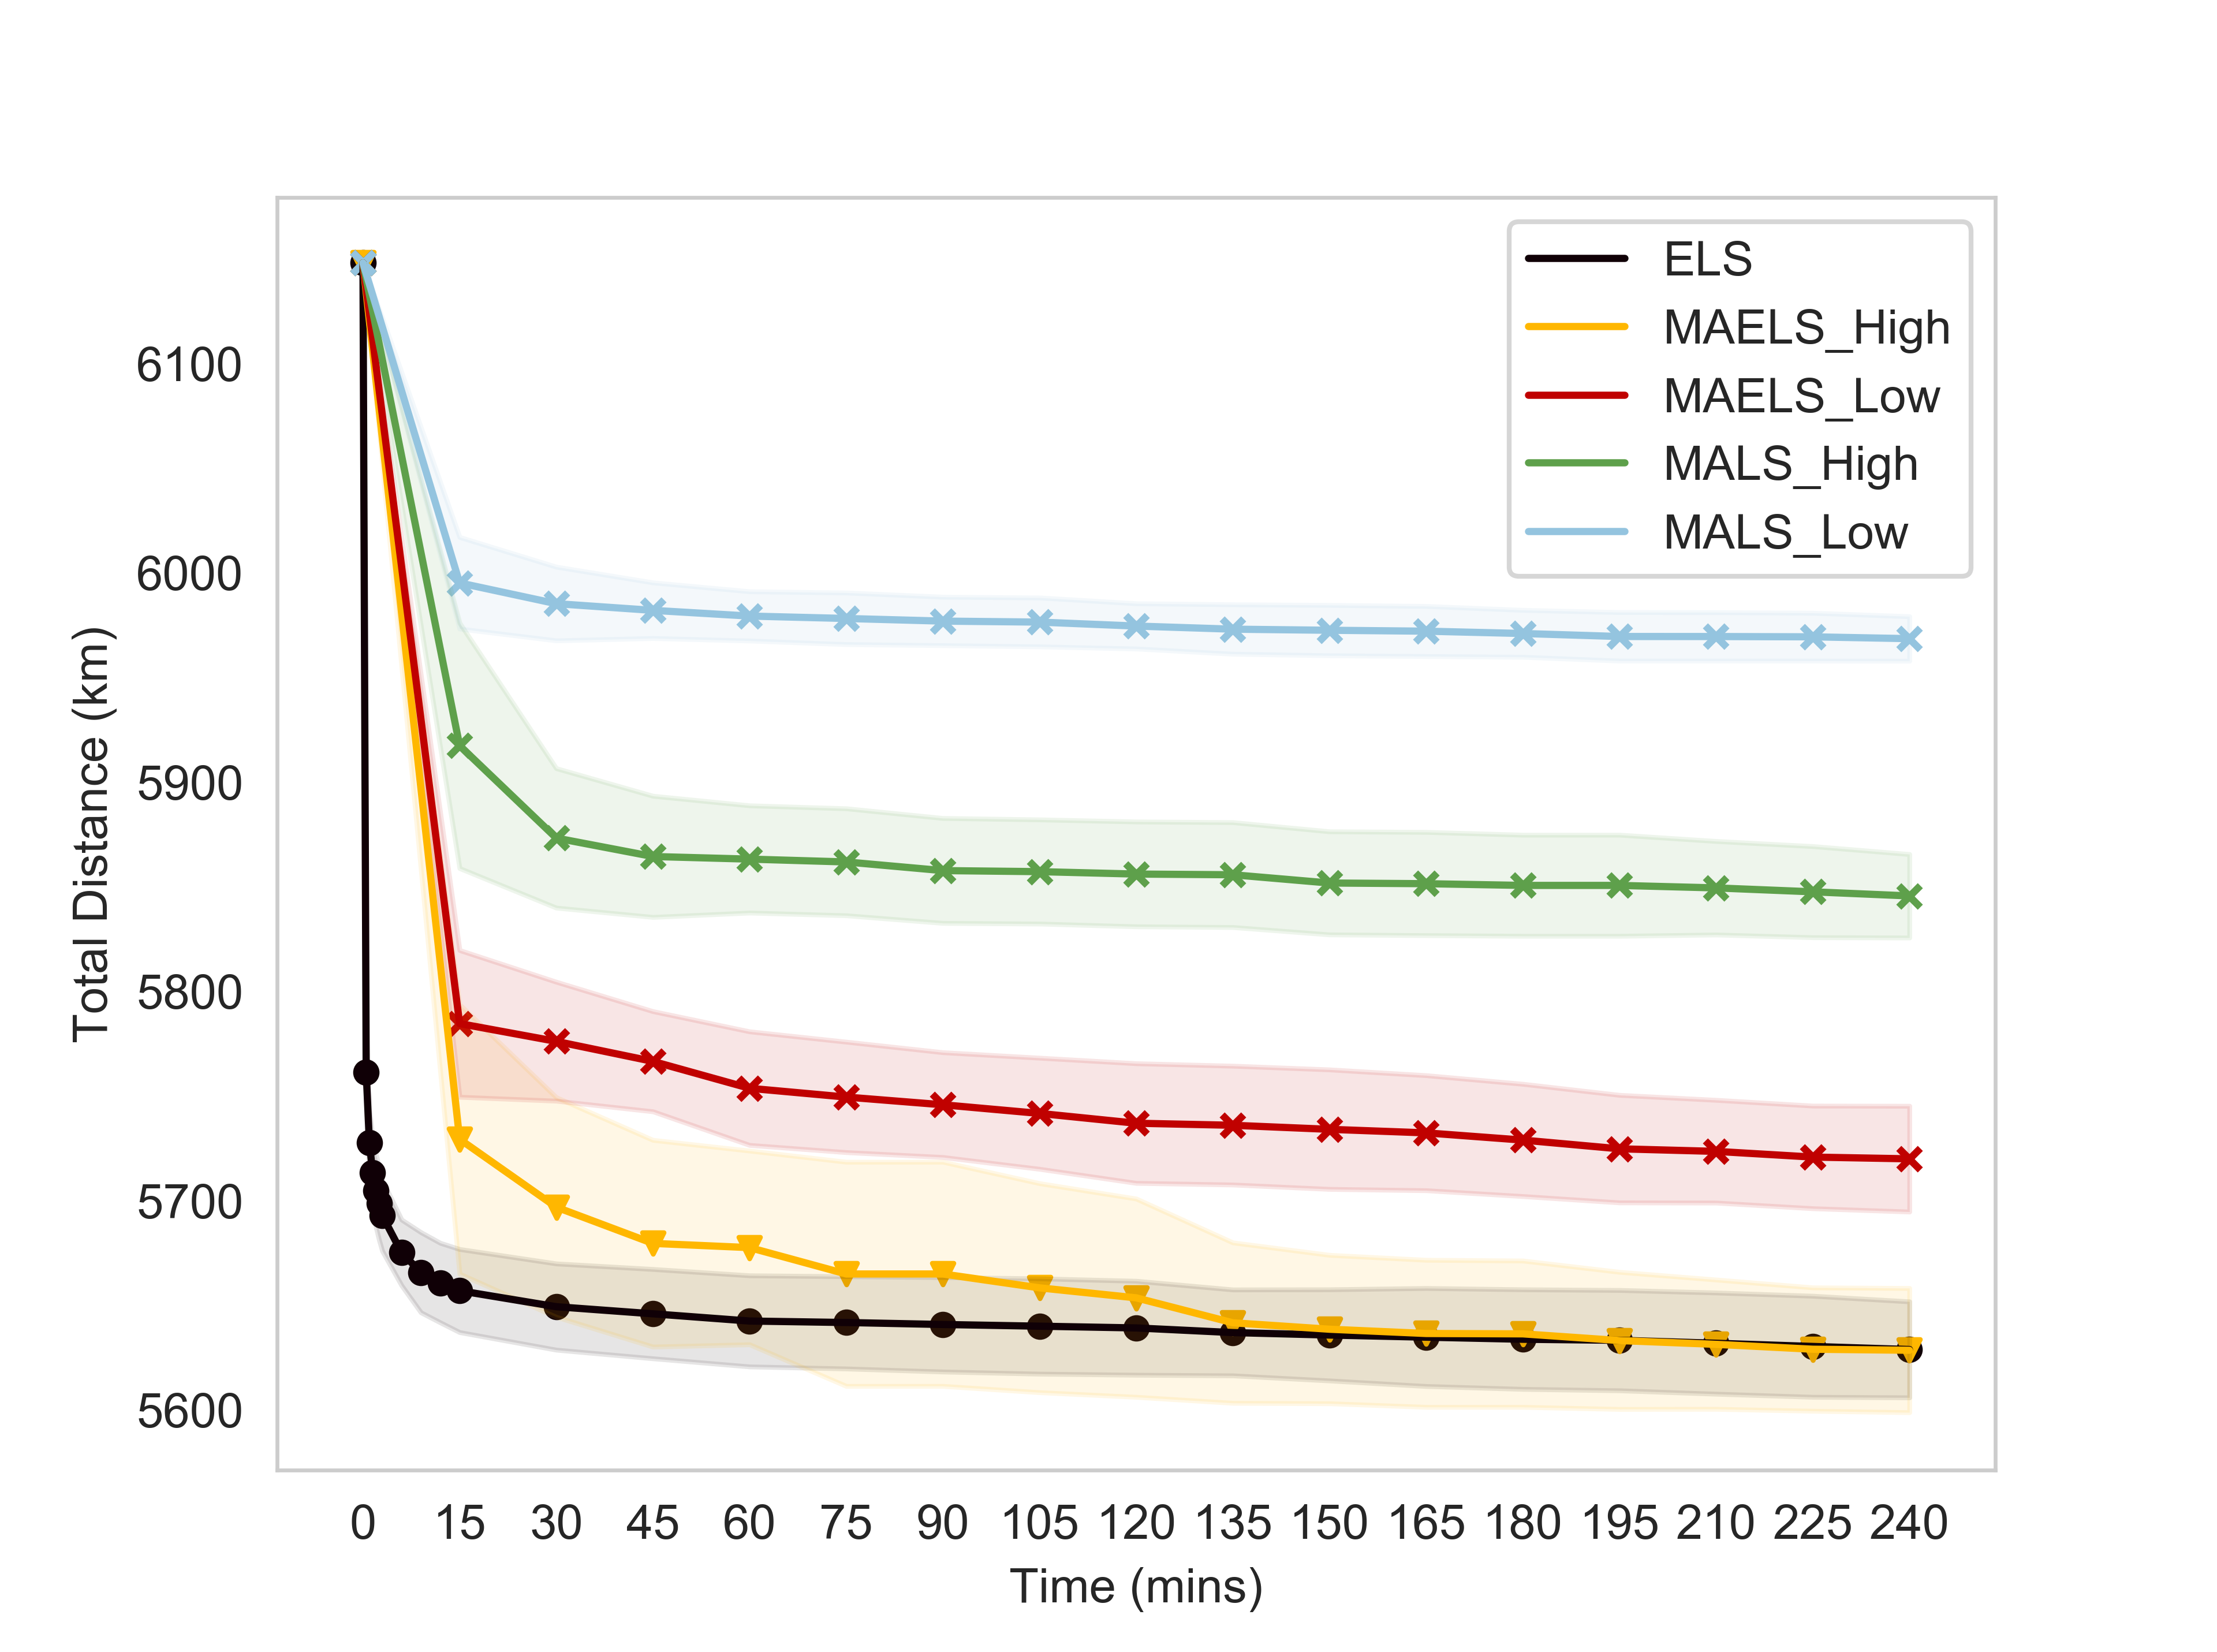
\includegraphics[width=1\columnwidth]{maels.png}}
    \end{subfloat}\\
    \begin{subfloat}[\label{fig:maels_12}
		ELS and MAELS with longer running time.]{
	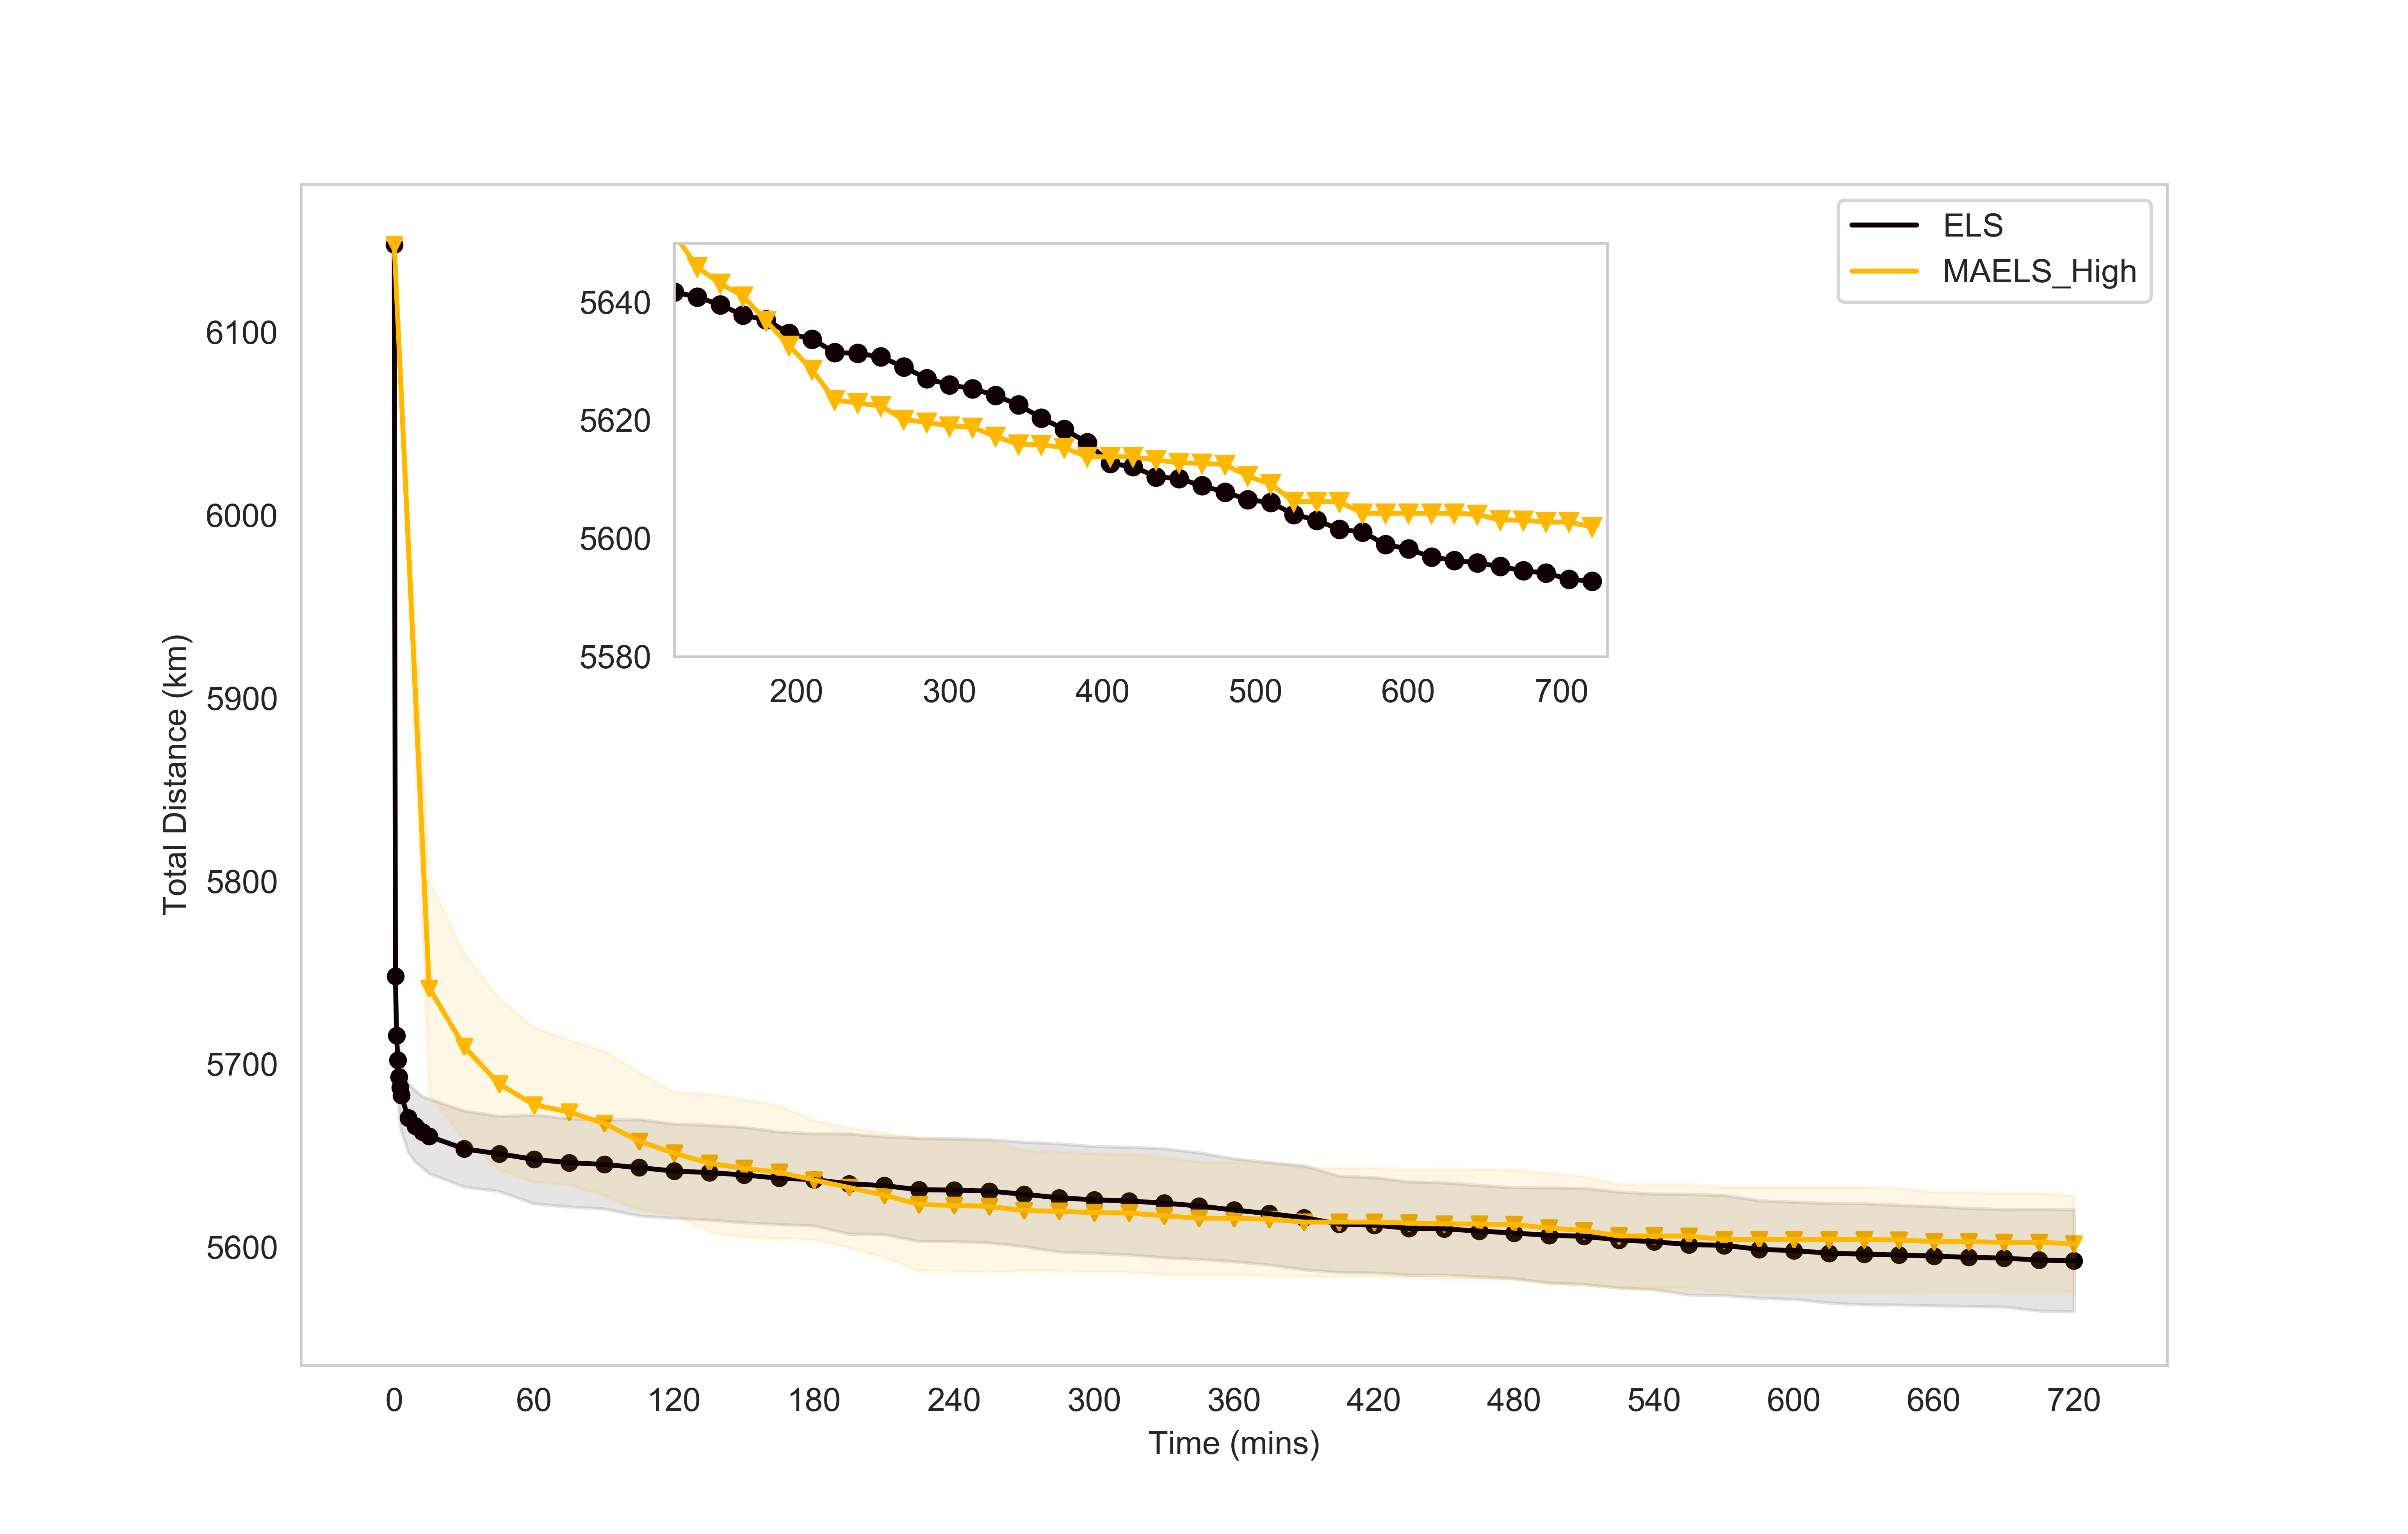
\includegraphics[width=1\columnwidth]{maels_12.png}}
    \end{subfloat}
    \caption{Total travel cost of ELS, compared with various local search algorithms. The shaded parts indicate the standard deviations.}
\end{figure}

\begin{table*}[htbp]
	\centering
	\caption{\label{data_comparison}
		The comparison between ELS, MALS and MAELS initialised with population of different diversity degree. ``BEST'' and ``AVG'' stand for the best and average distances obtained from 30 independent runs. ``STD'' stands for the standard deviation. The lowest average distance is marked with *. Results in bold (or underline) indicate that the corresponding algorithm is better (or worse) than ELS based on Wilcoxon rank-sum test with the level of significance 0.05.}
	\setlength{\tabcolsep}{4pt}
	\begin{tabular}{|c|ccc|ccc|ccc|ccc|ccc|}
		\hline
		\multirow{1}{*}{Time} & 
		\multicolumn{3}{c|}{ELS} &
		\multicolumn{3}{c|}{MAELS\_High} &
		\multicolumn{3}{c|}{MAELS\_Low} & 
		\multicolumn{3}{c|}{MALS\_High} &
		\multicolumn{3}{c|}{MALS\_Low}\\
		
		(mins)& BEST & AVG & STD & BEST & AVG & STD & BEST & AVG & STD & BEST & AVG & STD & BEST & AVG & STD  \\
		\hline
		0 & 6148.0 & 6148.0 & 0.0 & 6148.0 & 6148.0 & 0.0 & 6148.0 & 6148.0 & 0.0 & 6148.0 & 6148.0 & 0.0 & 6148.0 & 6148.0 & 0.0 \\
		15 & 5605.7 & 5656.9* & 19.9 & 5574.7 & \underline{5729.3} & 64.4 & 5704.2 & \underline{5784.5} & 35.1 & 5835.5 & \underline{5917.4} & 58.6 & 5943.2 & \underline{5995.1} & 521.9 \\
		30 & 5601.7 & 5649.3* & 20.6 & 5574.7 & \underline{5696.8} & 52.5 & 5704.2 & \underline{5776.0} & 28.4 & 5835.5 & \underline{5873.2} & 33.3 & 5943.2 & \underline{5985.2} & 17.6 \\
		45 & 5601.5 & 5645.9* & 21.3 & 5574.7 & \underline{5679.5} & 49.4 & 5704.2 & \underline{5766.5} & 23.9 & 5817.9 & \underline{5864.4} & 29.0 & 5943.2 & \underline{5982.0} & 13.3 \\
		60 & 5601.5 & 5642.4* & 21.8 & 5574.7 & \underline{5677.5} & 46.3 & 5660.8 & \underline{5753.6} & 27.1 & 5817.9 & \underline{5863.1} & 25.6 & 5943.2 & \underline{5979.3} & 11.8 \\
		75 & 5601.5 & 5641.7* & 22.0 & 5505.4 & \underline{5664.9} & 53.6 & 5660.8 & \underline{5749.4} & 26.4 & 5817.9 & \underline{5861.8} & 25.6 & 5943.2 & \underline{5978.1} & 12.3 \\
		90 & 5601.5 & 5640.8* & 22.6 & 5505.4 & \underline{5664.9} & 53.6 & 5660.8 & \underline{5745.7} & 25.0 & 5817.9 & \underline{5857.6} & 25.1 & 5943.2 & \underline{5976.9} & 11.6 \\
		105 & 5601.5 & 5634.0* & 22.8 & 5505.4 & 5658.3 & 49.9 & 5660.8 & \underline{5741.6} & 26.6 & 5817.9 & \underline{5857.1} & 24.9 & 5943.2 & \underline{5976.4} & 11.7 \\
		120 & 5599.3 & 5639.1* & 22.5 & 5505.4 & 5653.5 & 47.4 & 5660.8 & \underline{5736.9} & 28.6 & 5817.6 & \underline{5856.0} & 25.1 & 5943.2 & \underline{5974.5} & 10.8 \\
		135 & 5597.2 & 5636.9* & 20.5 & 5505.4 & 5641.6 & 38.3 & 5660.8 & \underline{5734.0} & 28.4 & 5817.6 & \underline{5855.7} & 25.1 & 5943.2 & \underline{5973.0} & 11.8 \\
		150 & 5583.4 & 5635.7* & 21.8 & 5505.4 & 5638.5 & 35.5 & 5660.8 & \underline{5734.0} & 28.6 & 5812.6 & \underline{5851.7} & 24.6 & 5943.2 & \underline{5972.5} & 12.0 \\
		165 & 5569.2 & 5634.7* & 23.4 & 5505.4 & 5636.5 & 35.1 & 5660.8 & \underline{5732.3} & 27.5 & 5812.6 & \underline{5851.4} & 24.7 & 5943.2 & \underline{5972.0} & 12.0 \\
		180 & 5568.5 & 5633.7* & 23.8 & 5505.4 & 5636.3 & 35.0 & 5660.8 & \underline{5728.9} & 26.8 & 5812.6 & \underline{5850.6} & 24.2 & 5943.2 & \underline{5970.9} & 11.2 \\
		195 & 5568.5 & 5633.2* & 24.0 & 5505.4 & 5633.1 & 32.8 & 5660.8 & \underline{5724.7} & 25.7 & 5812.6 & \underline{5850.6} & 24.2 & 5943.2 & \underline{5969.5} & 11.6 \\
		210 & 5568.5 & 5631.8 & 24.2 & 5505.4 & 5631.3* & 30.9 & 5660.8 & \underline{5723.5} & 24.6 & 5812.6 & \underline{5849.4} & 22.3 & 5943.2 & \underline{5969.5} & 11.6 \\
		225 & 5568.5 & 5630.3 & 24.2 & 5505.4 & 5628.9* & 29.5 & 5660.8 & \underline{5720.8} & 24.5 & 5812.6 & \underline{5847.5} & 21.8 & 5943.2 & \underline{5969.3} & 11.4 \\
		240 & 5568.5 & 5628.8 & 22.9 & 5505.4 & 5628.5* & 29.7 & 5660.8 & \underline{5719.9} & 25.3 & 5812.6 & \underline{5845.5} & 19.9 & 5943.2 & \underline{5968.5} & 10.6 \\
		\hline
	\end{tabular}
\end{table*}


\subsection{Discussion}\label{sec:om_disscussion}
MAELS cannot guarantee that the optimised solutions do not exceed the maximum working time of vehicles. Nevertheless, a small amount of extra working time is acceptable as the current model does not take into account the uncertainties in real life, which may lead to longer or shorter service time. Additionally, including stricter constraints, such as refusing to add infeasible individuals to the population, is possible but not necessary. Since it may reduce the ability of MAELS to jump out of the local optimal, thereby making its optimisation effect worse. On the other hand, relaxing the constraints of the maximum working time of vehicles (e.g., changing from 8 hours to 8.5 hours) in ELS/MAELS may increase the probability of rejecting better solutions. Some favourable solutions may need to be obtained by the optimisation on infeasible initial solutions. MAELS may speed up its optimisation if the best individual in the population is always selected as one of the parents for crossover.


\def\keepforlater{
\section{Discussion}\label{sec:all_discussion}

\todo[inline]{This part can be deleted.}

In this section, some enlightenments obtained from this research are discussed as below:
\begin{enumerate}
	\item VRP and facility location problem (FLP) should be considered together as much as possible in real application. Because on the one hand, the total travel distance of the solution without depots and disposal facilities is 1,300 $km$ shorter than the total travel distance of the solution with depots and disposal facilities on average, on the other hand the location of some disposal facilities is very unreasonable in the dataset used in this paper (See in Figure~\ref{fig:dataset}).
	\item For some extremely complex problems, "Greedy Strategy" can help you find feasible solution within a very short time though it may not find the optimal solution. Additionally, some traversals with short time cost may help improve the solution obtained by the greedy strategy, likes BSIM in this paper.
\end{enumerate}
}


%===========================  第  五  段  ===================================
\section{Conclusion}\label{sec:conclusion}
In this paper, we formulate a multi-depot multi-disposal-facility multi-trip capacitated vehicle routing problem (M3CVRP) for a real-world large-scale waste collection problem with many constraints that no existing work has ever solved such problem of this size. We design a heuristic-assisted solution initialisation approach (HaSI) for generating feasible initial solutions of high quality, combining the idea of greedy strategy with the consideration of tight capacity and working time. Due to the characteristics of solution representation during optimisation, a better insertion method, backspacing insertion method (BSIM), is proposed. Moreover, two novel search operators considering regional information and one novel search operators helping to jump out of the local optimum have been designed and embedded in an extended local search (ELS) algorithm, as well as a memetic algorithm with ELS (MAELS) to optimise feasible initial solutions further. The HaSI is compared with the adaptations of Clarke and Wright Savings Algorithm. Experimental study shows that HaSI is capable of generating high-quality and diverse initial solutions. By re-allocating the depots and disposal facilities on these initial solutions, BSIM significantly reduces most of the solutions. Compared with MALS, a sophisticated memetic algorithm, ELS can efficiently find good solutions. In particular, ELS can rapidly find high-quality solutions in a very short period, which makes it suitable for real-life applications. For some incredibly complex problems, a greedy strategy can help to find feasible solutions within a very short time though it may not find the optimal solution. Additionally, some additional traversals within a short time may help to improve the solution obtained by the greedy strategy, like BSIM proposed in this paper.

%when optimisation has just started. 
%However, as the optimisation time increases, the gap between the optimisation effects of ELS and MAELS is getting smaller and smaller.

There are several potential research directions as future work. Designing a search operator or heuristic to adapt the number of vehicles in the optimisation process needs to be researched.  In order to speed up the optimisation of MAELS, MAELS can include heuristics to apply ELS to only the best feasible solution or those ''promising'' (e.g., with low cost and feasible) solutions~\cite{tang2009memetic}. %Moreover, VRP and facility location problem should be considered together as much as possible in real-life application. Because on the one hand, the total travel distance of the solution without depots and disposal facilities is 1,300 $km$ shorter than the total travel distance of the solution with depots and disposal facilities on average, on the other hand the location of some disposal facilities is very unreasonable in the dataset used in this paper (cf. Figure~\ref{fig:dataset}).

%\subsection*{Future Work}
 %From the experimental results, we notice that the strategy for choosing a depot in HaSI needs improvements. How to choose the best combination and parameter setting of these search operators in ELS is worth investigating. 
%Additionally, 

%
% ---- Bibliography ----
%
\balance
\bibliographystyle{IEEEtran}
\bibliography{wasteCollection}

\end{document}

